\documentclass[final,3p,times]{elsarticle}
\usepackage[utf8]{inputenc}
\usepackage{amssymb}
\usepackage{float}
\usepackage{placeins}
\usepackage{amsmath}
\usepackage{booktabs}
\usepackage{textcomp}
\usepackage{multirow}
\usepackage{threeparttable}
\usepackage{siunitx}
\usepackage[table]{xcolor}
\usepackage{xurl}
\usepackage{hyperref}
\usepackage{pgfplots}
\usepgfplotslibrary{colormaps,groupplots,statistics}
\pgfplotsset{compat=1.18}
\usepackage{tikz}
\usetikzlibrary{shapes,arrows.meta,positioning,fit,backgrounds,calc}
\setlength{\marginparwidth}{2cm}
\usepackage{todonotes}
\usepackage{alltt}
\graphicspath{{./}{Images/}}
% --- Inline figure definitions (formerly figures.tex) ---
\setlength{\textfloatsep}{10pt plus 2pt minus 4pt}   % Distance between top/bottom float and text
\setlength{\floatsep}{8pt plus 2pt minus 2pt}       % Distance between two floats
\setlength{\intextsep}{10pt plus 2pt minus 2pt}     % Distance between inline float and text
\renewcommand{\floatpagefraction}{0.7}
\renewcommand{\textfraction}{0.15}
\renewcommand{\topfraction}{0.85}
\renewcommand{\bottomfraction}{0.65}

\newcommand{\plotCriterionMAEByModel}{%
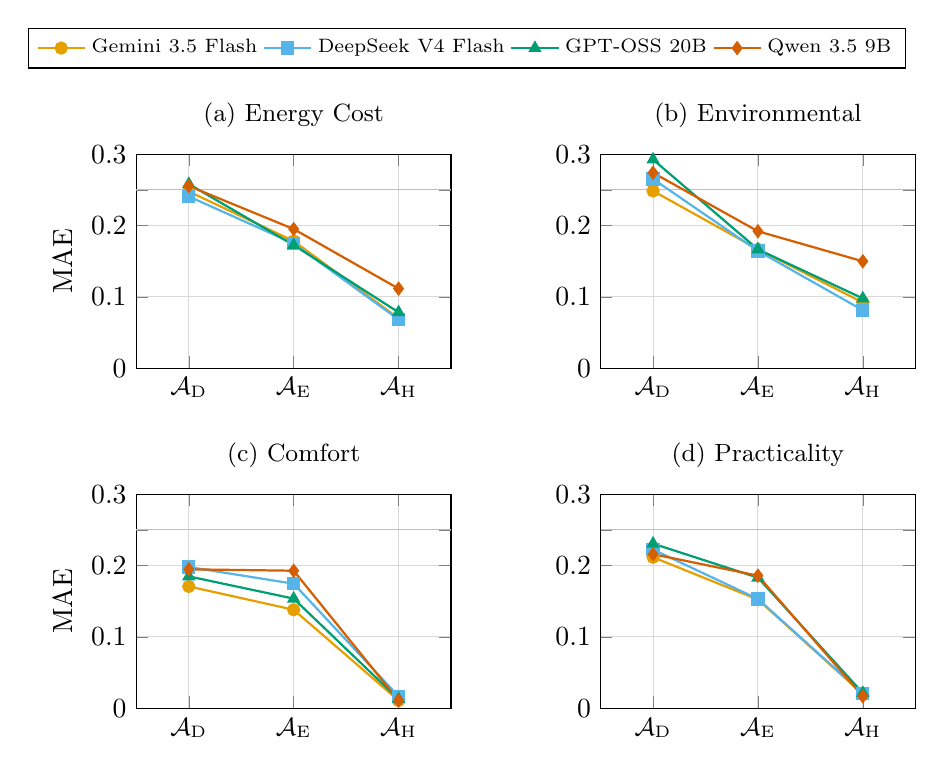
\begin{tikzpicture}
\begin{groupplot}[
    group style={group size=2 by 2, horizontal sep=1.9cm, vertical sep=1.6cm},
    width=0.46\textwidth, height=4.3cm,
    xtick={1,2,3}, xticklabels={$\mathcal{A}_{\text{D}}$,$\mathcal{A}_{\text{E}}$,$\mathcal{A}_{\text{H}}$},
    xticklabel style={font=\small},
    enlarge x limits=0.25,
    grid=major, grid style={gray!30}, ymajorgrids=true,
    extra y ticks={0.25,0.5,0.75},
    extra y tick style={grid=major, grid style={gray!50}},
    extra y tick labels={},
    legend style={font=\scriptsize, at={(1.05,1.4)}, anchor=south, legend columns=4},
    legend cell align={left},
    every axis plot/.append style={thick, mark size=2pt},
]
\nextgroupplot[ylabel={MAE}, ymin=0, ymax=0.3,
    title={\small (a) Energy Cost}, title style={font=\small}]
\addplot[mark=*, colorGemini]   coordinates {(1,0.2477) (2,0.1782) (3,0.0698)};
\addplot[mark=square*, colorDeepSeek] coordinates {(1,0.2407) (2,0.1748) (3,0.0683)};
\addplot[mark=triangle*, colorGPTOSS] coordinates {(1,0.2581) (2,0.1725) (3,0.0783)};
\addplot[mark=diamond*, colorQwen] coordinates {(1,0.2554) (2,0.1950) (3,0.1115)};
\legend{Gemini 3.5 Flash, DeepSeek V4 Flash, GPT-OSS 20B, Qwen 3.5 9B}
\nextgroupplot[ylabel={}, ymin=0, ymax=0.3,
    title={\small (b) Environmental}, title style={font=\small}]
\addplot[mark=*, colorGemini]   coordinates {(1,0.2484) (2,0.1667) (3,0.0921)};
\addplot[mark=square*, colorDeepSeek] coordinates {(1,0.2652) (2,0.1644) (3,0.0812)};
\addplot[mark=triangle*, colorGPTOSS] coordinates {(1,0.2924) (2,0.1665) (3,0.0978)};
\addplot[mark=diamond*, colorQwen] coordinates {(1,0.2739) (2,0.1919) (3,0.1498)};
\nextgroupplot[ylabel={MAE}, ymin=0, ymax=0.3,
    title={\small (c) Comfort}, title style={font=\small}]
\addplot[mark=*, colorGemini]   coordinates {(1,0.1707) (2,0.1380) (3,0.0108)};
\addplot[mark=square*, colorDeepSeek] coordinates {(1,0.1979) (2,0.1745) (3,0.0167)};
\addplot[mark=triangle*, colorGPTOSS] coordinates {(1,0.1848) (2,0.1536) (3,0.0127)};
\addplot[mark=diamond*, colorQwen] coordinates {(1,0.1947) (2,0.1927) (3,0.0108)};
\nextgroupplot[ylabel={}, ymin=0, ymax=0.3,
    title={\small (d) Practicality}, title style={font=\small}]
\addplot[mark=*, colorGemini]   coordinates {(1,0.2116) (2,0.1523) (3,0.0197)};
\addplot[mark=square*, colorDeepSeek] coordinates {(1,0.2224) (2,0.1531) (3,0.0208)};
\addplot[mark=triangle*, colorGPTOSS] coordinates {(1,0.2307) (2,0.1830) (3,0.0213)};
\addplot[mark=diamond*, colorQwen] coordinates {(1,0.2159) (2,0.1858) (3,0.0168)};
\end{groupplot}
\end{tikzpicture}%
}

\newcommand{\plotDecisionTypeByModel}{%
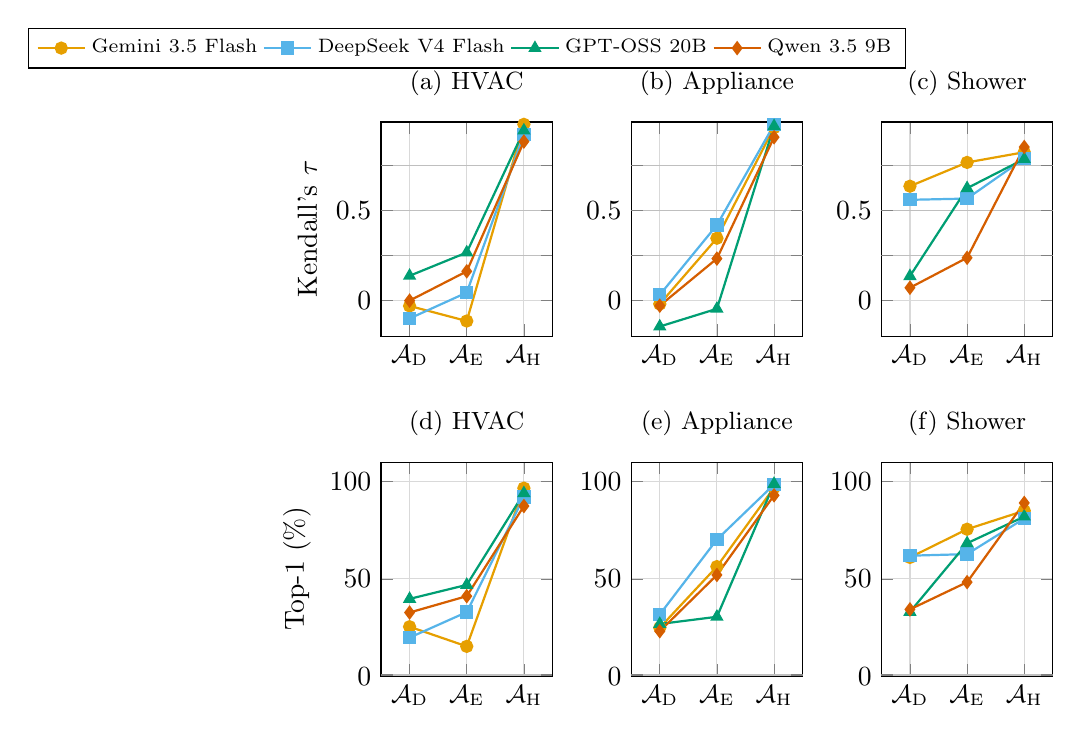
\begin{tikzpicture}
\begin{groupplot}[
    group style={group size=3 by 2, vertical sep=1.6cm},
    width=0.31\textwidth, height=4.3cm,
    xtick={1,2,3}, xticklabels={$\mathcal{A}_{\text{D}}$,$\mathcal{A}_{\text{E}}$,$\mathcal{A}_{\text{H}}$},
    xticklabel style={font=\small},
    enlarge x limits=0.25,
    grid=major, grid style={gray!30}, ymajorgrids=true,
    extra y ticks={0.25,0.5,0.75},
    extra y tick style={grid=major, grid style={gray!50}},
    extra y tick labels={},
    legend style={font=\scriptsize, at={(0.5,1.25)}, anchor=south, legend columns=4},
    legend cell align={left},
    every axis plot/.append style={thick, mark size=2pt},
]
\nextgroupplot[ylabel={Kendall's $\tau$}, ymin=-0.2, ymax=0.99,
    title={\small (a) HVAC}, title style={font=\small}]
\addplot[mark=*, colorGemini]   coordinates {(1,-0.0324) (2,-0.1162) (3,0.9772)};
\addplot[mark=square*, colorDeepSeek] coordinates {(1,-0.1021) (2,0.0419) (3,0.9197)};
\addplot[mark=triangle*, colorGPTOSS] coordinates {(1,0.1352) (2,0.2647) (3,0.9428)};
\addplot[mark=diamond*, colorQwen] coordinates {(1,-0.0027) (2,0.1600) (3,0.8813)};
\legend{Gemini 3.5 Flash, DeepSeek V4 Flash, GPT-OSS 20B, Qwen 3.5 9B}
\nextgroupplot[ylabel={}, ymin=-0.2, ymax=0.99,
    title={\small (b) Appliance}, title style={font=\small}]
\addplot[mark=*, colorGemini]   coordinates {(1,-0.0215) (2,0.3441) (3,0.9590)};
\addplot[mark=square*, colorDeepSeek] coordinates {(1,0.0293) (2,0.4174) (3,0.9754)};
\addplot[mark=triangle*, colorGPTOSS] coordinates {(1,-0.1467) (2,-0.0482) (3,0.9672)};
\addplot[mark=diamond*, colorQwen] coordinates {(1,-0.0309) (2,0.2308) (3,0.9056)};
\nextgroupplot[ylabel={}, ymin=-0.2, ymax=0.99,
    title={\small (c) Shower}, title style={font=\small}]
\addplot[mark=*, colorGemini]   coordinates {(1,0.6333) (2,0.7655) (3,0.8222)};
\addplot[mark=square*, colorDeepSeek] coordinates {(1,0.5576) (2,0.5645) (3,0.7867)};
\addplot[mark=triangle*, colorGPTOSS] coordinates {(1,0.1333) (2,0.6222) (3,0.7845)};
\addplot[mark=diamond*, colorQwen] coordinates {(1,0.0689) (2,0.2355) (3,0.8511)};
\nextgroupplot[ylabel={Top-1 (\%)}, ymin=0, ymax=110,
    title={\small (d) HVAC}, title style={font=\small}]
\addplot[mark=*, colorGemini]   coordinates {(1,25.4) (2,15.3) (3,96.6)};
\addplot[mark=square*, colorDeepSeek] coordinates {(1,19.8) (2,32.9) (3,92.0)};
\addplot[mark=triangle*, colorGPTOSS] coordinates {(1,39.7) (2,46.9) (3,94.0)};
\addplot[mark=diamond*, colorQwen] coordinates {(1,32.7) (2,41.1) (3,87.4)};
\nextgroupplot[ylabel={}, ymin=0, ymax=110,
    title={\small (e) Appliance}, title style={font=\small}]
\addplot[mark=*, colorGemini]   coordinates {(1,24.9) (2,56.3) (3,96.9)};
\addplot[mark=square*, colorDeepSeek] coordinates {(1,31.7) (2,70.2) (3,98.5)};
\addplot[mark=triangle*, colorGPTOSS] coordinates {(1,26.8) (2,30.5) (3,98.8)};
\addplot[mark=diamond*, colorQwen] coordinates {(1,23.1) (2,52.0) (3,92.9)};
\nextgroupplot[ylabel={}, ymin=0, ymax=110,
    title={\small (f) Shower}, title style={font=\small}]
\addplot[mark=*, colorGemini]   coordinates {(1,61.0) (2,75.5) (3,85.0)};
\addplot[mark=square*, colorDeepSeek] coordinates {(1,61.9) (2,62.7) (3,81.0)};
\addplot[mark=triangle*, colorGPTOSS] coordinates {(1,33.0) (2,68.3) (3,82.0)};
\addplot[mark=diamond*, colorQwen] coordinates {(1,34.3) (2,48.3) (3,89.0)};
\end{groupplot}
\end{tikzpicture}%
}

\newcommand{\plotRagAblation}{%
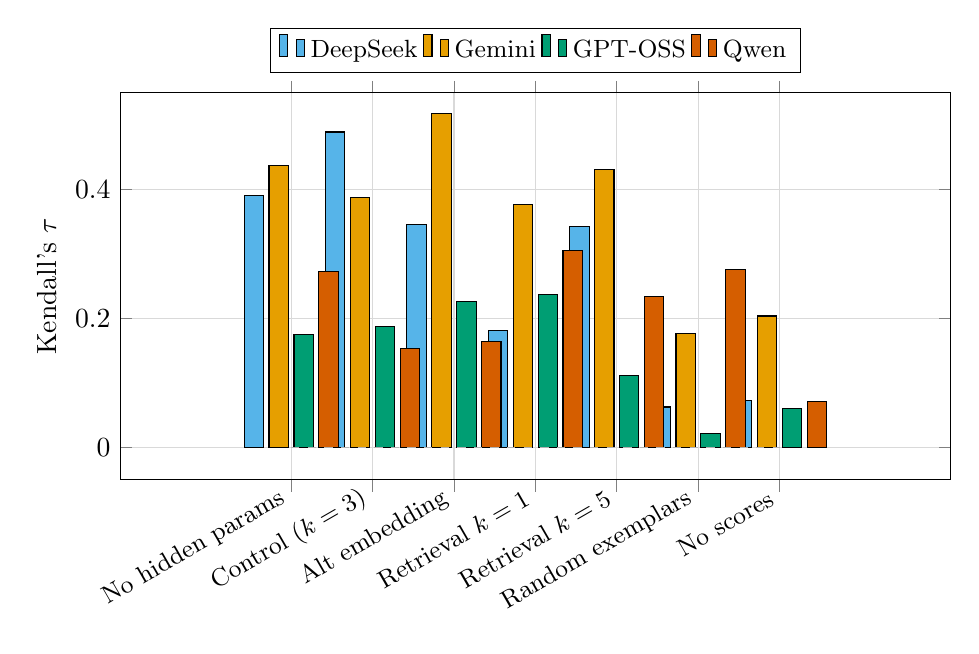
\begin{tikzpicture}
\begin{axis}[
    width=\textwidth, height=6.5cm,
    ylabel={Kendall's $\tau$},
    symbolic x coords={No hidden params,Control ($k=3$),Alt embedding,Retrieval $k=1$,Retrieval $k=5$,Random exemplars,No scores},
    xtick=data,
    xticklabel style={rotate=30, anchor=east, font=\small, align=center},
    enlarge x limits=0.35,
    bar width=7pt,
    ybar,
    ymin=-0.05, ymax=0.55,
    legend style={font=\small, at={(0.5,1.05)}, anchor=south, legend columns=4},
    legend cell align={left},
    grid=major,
    grid style={gray!30},
    ymajorgrids=true,
]
\addplot[fill=colorDeepSeek] coordinates {
    (No hidden params,0.391)
    (Control ($k=3$),0.489)
    (Alt embedding,0.346)
    (Retrieval $k=1$,0.182)
    (Retrieval $k=5$,0.342)
    (Random exemplars,0.063)
    (No scores,0.073)
};
\addplot[fill=colorGemini] coordinates {
    (No hidden params,0.437)
    (Control ($k=3$),0.387)
    (Alt embedding,0.517)
    (Retrieval $k=1$,0.377)
    (Retrieval $k=5$,0.431)
    (Random exemplars,0.177)
    (No scores,0.204)
};
\addplot[fill=colorGPTOSS] coordinates {
    (No hidden params,0.175)
    (Control ($k=3$),0.187)
    (Alt embedding,0.227)
    (Retrieval $k=1$,0.237)
    (Retrieval $k=5$,0.112)
    (Random exemplars,0.022)
    (No scores,0.061)
};
\addplot[fill=colorQwen] coordinates {
    (No hidden params,0.273)
    (Control ($k=3$),0.154)
    (Alt embedding,0.165)
    (Retrieval $k=1$,0.306)
    (Retrieval $k=5$,0.234)
    (Random exemplars,0.276)
    (No scores,0.071)
};
\addplot[dashed, gray!60, sharp plot, update limits=false] coordinates {
    (No hidden params,0) (No scores,0)
};
\legend{DeepSeek,Gemini,GPT-OSS,Qwen}
\end{axis}
\end{tikzpicture}%
}

\newcommand{\plotSensitivityTau}{%
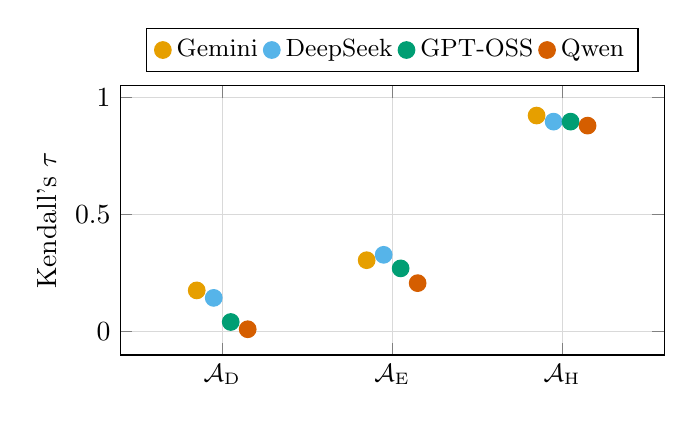
\begin{tikzpicture}
\begin{axis}[
    width=0.7\textwidth, height=5cm,
    ylabel={Kendall's $\tau$},
    xtick={1,2,3},
    xticklabels={$\mathcal{A}_{\text{D}}$,$\mathcal{A}_{\text{E}}$,$\mathcal{A}_{\text{H}}$},
    xticklabel style={font=\small},
    xmin=0.4, xmax=3.6,
    ymin=-0.1, ymax=1.05,
    grid=major,
    grid style={gray!30},
    ymajorgrids=true,
    legend style={font=\small, at={(0.5,1.05)}, anchor=south, legend columns=4},
    legend cell align={left},
]
\addplot[only marks, mark=*, mark size=3pt, color=colorGemini] coordinates {
    (0.85, 0.176) (1.85, 0.305) (2.85, 0.923)
};
\addplot[only marks, mark=*, mark size=3pt, color=colorDeepSeek] coordinates {
    (0.95, 0.144) (1.95, 0.328) (2.95, 0.897)
};
\addplot[only marks, mark=*, mark size=3pt, color=colorGPTOSS] coordinates {
    (1.05, 0.041) (2.05, 0.270) (3.05, 0.897)
};
\addplot[only marks, mark=*, mark size=3pt, color=colorQwen] coordinates {
    (1.15, 0.010) (2.15, 0.207) (3.15, 0.880)
};
\legend{Gemini, DeepSeek, GPT-OSS, Qwen}
\end{axis}
\end{tikzpicture}%
}

% --- End inline figure definitions ---
\definecolor{colorPure}{RGB}{180,180,180}
\definecolor{colorRAG}{RGB}{100,149,200}
\definecolor{colorLLMParameterizedReferenceScoring}{RGB}{31,73,125}
\definecolor{colorGemini}{HTML}{E69F00}
\definecolor{colorDeepSeek}{HTML}{56B4E9}
\definecolor{colorGPTOSS}{HTML}{009E73}
\definecolor{colorQwen}{HTML}{D55E00}
\journal{Environmental Modelling \& Software}
\begin{document}
\begin{frontmatter}
\title{Benchmarking LLM Integration Strategies for MCDA-Assisted Household Energy Decision Support}
\author{Ahaan Nigam\corref{cor1}}
\cortext[cor1]{Corresponding author.}
\ead{ishaannigam27@gmail.com}
\affiliation{organization={Downingtown East High School},
            city={Exton},
            state={Pennsylvania},
            country={USA}}
\author{River Huang}
\affiliation{organization={Paul Scherrer Institut},
            city={Villigen},
            state={Aargau},
            country={Switzerland}}
\begin{abstract}
The residential sector is a major source of global CO\textsubscript{2} emissions, yet most households rely on biased decisions rather than tailored ones. Multi-Attribute Value Theory (MAVT) offers a rigorous Multi-Criteria Decision Analysis (MCDA) method to reduce emissions, but building MCDAs requires expertise that limits household adoption. This study contributes an evaluation framework and an open reference implementation for LLM-fronted MCDA in residential energy, and uses it to compare three architectures: Direct LLM Scoring ($\mathcal{A}_{\text{D}}$~), Example-Guided LLM Scoring ($\mathcal{A}_{\text{E}}$~), and LLM-Parameterized Reference Scoring ($\mathcal{A}_{\text{H}}$~), which extracts engineering parameters for a deterministic reference calculator. Reference calculators benchmarked MAVT scores across HVAC, appliance, and shower decisions. Over 195 scenarios and four models, $\mathcal{A}_{\text{H}}$ achieved a Kendall's tau of 0.880--0.923 and 89.7--93.1\% Top-1 accuracy (four-model means 0.899 and 91.3\%); $\mathcal{A}_{\text{E}}$ scored 0.207--0.328 and 47.0--54.5\% (means 0.277 and 49.2\%), and $\mathcal{A}_{\text{D}}$ 0.010--0.176 and 30.0--36.7\% (means 0.093 and 34.1\%). Two non-LLM baselines on the same scenarios place those figures: a fixed-default parameter substitution into the same calculator reached tau 0.614 and 70.3\% Top-1, and nearest-neighbour exemplar copying 0.371 and 56.9\%, so only $\mathcal{A}_{\text{H}}$ beat both. $\mathcal{A}_{\text{H}}$ also compressed model capability: its tau spanned 0.043 across a 45$\times$ range of model cost, against 0.166 for $\mathcal{A}_{\text{D}}$. Under a seven-vector weight sensitivity analysis, $\mathcal{A}_{\text{H}}$ leads $\mathcal{A}_{\text{E}}$ in all 28 model $\times$ vector cells, while $\mathcal{A}_{\text{E}}$'s lead over $\mathcal{A}_{\text{D}}$ reverses in two MEREC cells; three ablation suites separate retrieval depth, prompt wording, and parameter provenance. The calculators, scenario corpus, and analysis code are released. Accuracy means agreement with a deterministic reference calculator, not measured household energy data.\end{abstract}
\begin{keyword}
Large language models \sep Multi-criteria decision analysis \sep Multi-Attribute Value Theory \sep Household energy \sep Decision support systems \sep Retrieval-Augmented Generation \sep Sustainability
\end{keyword}
\end{frontmatter}

\section{Introduction}
\label{sec1}
The average U.S.\ household emits roughly 8{,}744 pounds of CO\textsubscript{2}e and consumes about 10{,}791 kWh of electricity each year \cite{epa_household2024,eia_faq_electricity2024}. Globally, residential energy consumption has grown at roughly 1\% per year since 2000, driven by increasing household sizes and comfort demands in emerging economies \cite{GONZALEZTORRES2022112428}. However, a considerable portion of this usage is adjustable, creating opportunities to reduce both household cost and environmental impact \cite{dietz2009,ohler2020}.

Tools that combine optimization, behavioral insight, and decision support can close part of that gap, but only if they are usable without specialized training. Certain frameworks, such as Multi-Criteria Decision Analysis (MCDA), can be used to choose an optimal balance of factors that matter to users \cite{huang2011}. In theory, they would allow environmentally optimal choices consistently accross fields. However, constructing an MCDA model requires defining alternatives, criteria, weights, value functions, and normalization rules, making it impractical for routine household decisions.

It has been proposed in the past that LLMs could be used to automate this process, thus making it practical for household decisions. Without knowing how accurate these LLMs are as experts, it is unclear whether this would be a beneficial or detrimental idea.

Modern LLMs carry general knowledge about the energy use and carbon intensity of common products and behaviours, and many systems can retrieve additional information at inference time. They have not, however, been tested extensively for their abilities as MCDA designers \cite{svoboda2024,icaart26}. It is reasonable to say that they are not consistent decision makers \cite{wang2024fairescalers,li2026scoringbias}. Still, the amount of assistance needed to improve their designer ability to a reasonably accurate level has not been tested either. This study addresses that gap by benchmarking the three architectures across three household energy decision types, holding the model and the MAVT weighting constant for each architecture.

Thus, we aimed to answer the following questions: Which LLM-assisted architecture most accurately reproduces a ground truth produced ranking for rapid household decision support?
Then, how consistently does the architecture ranking hold across models of varying capability?

\section{Literature Review}
\label{sec:lit-review}

\subsection{Household Energy Decision-Making and Adoption Barriers}

Globally, residential buildings account for 18\% of CO\textsubscript{2} emissions \cite{GONZALEZTORRES2022112428}; in the United States, the residential sector consumed 11.8 quadrillion BTU (3{,}458 TWh) of delivered energy in 2022 and accounted for roughly 20\% of national energy-related CO\textsubscript{2} emissions \cite{eia2022,goldstein2020}. If the U.S.\ residential sector were a country, its emissions would rank sixth globally, comparable to Brazil and larger than Germany \cite{goldstein2020}.

\cite{dietz2009} estimated that household behavioral changes could reduce U.S.\ emissions by approximately 451 MtCO\textsubscript{2}e annually, savings that remain available to the average household today. That potential concentrates in a few areas: HVAC systems alone account for roughly a third of global residential energy consumption \cite{GONZALEZTORRES2022112428}.

\begin{figure}[H]
	\centering
	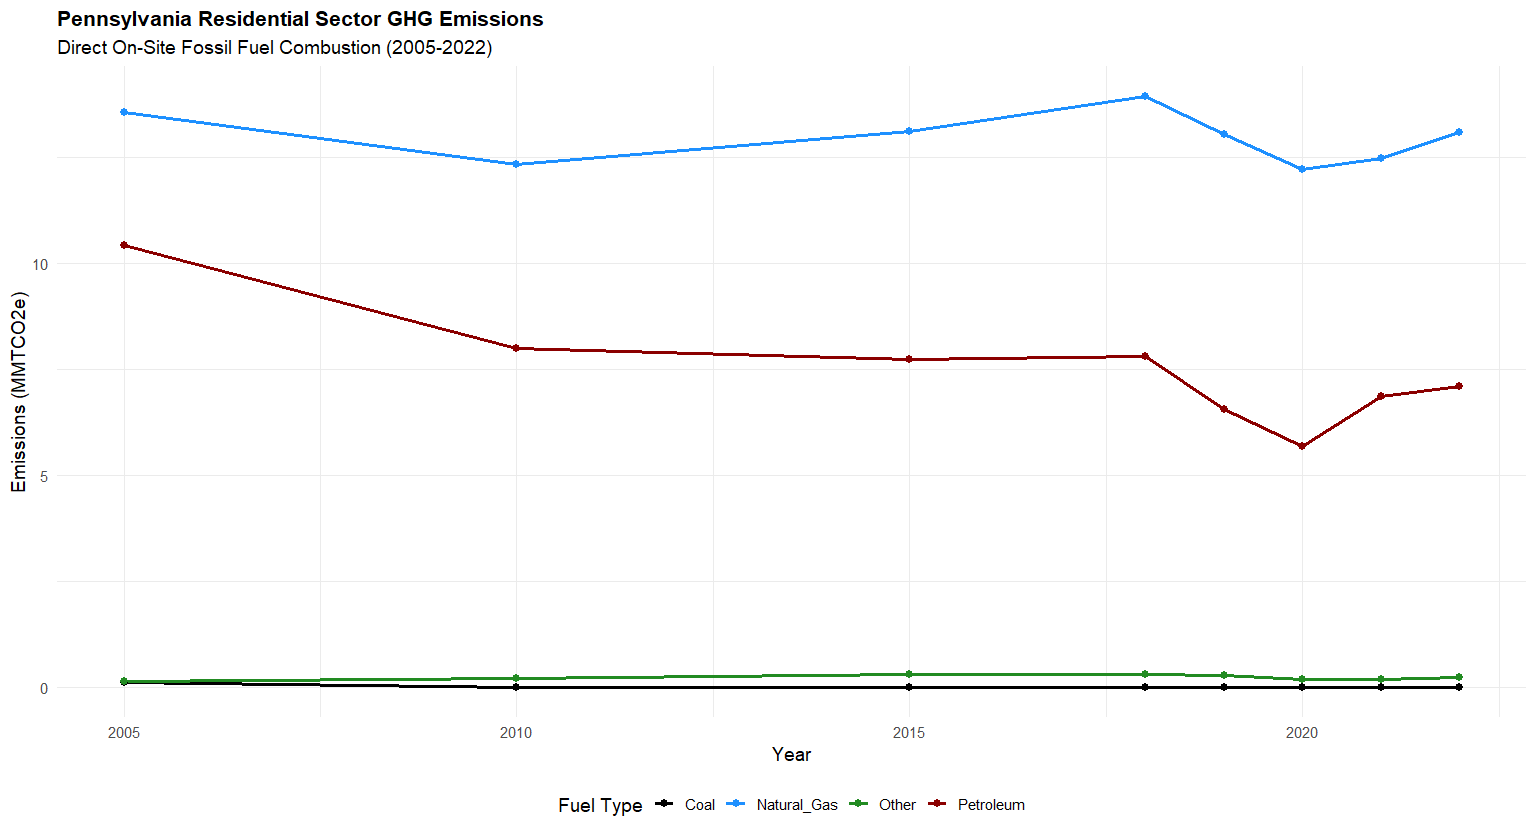
\includegraphics[width=1\textwidth]{PA_Residential_Emissions.png}
  \caption{Residential emissions, 2005--2022 \cite{eia2022,goldstein2020}.}
\label{fig:pa_residential_emissions}
\end{figure}

Figure~\ref{fig:pa_residential_emissions} shows that residential emissions remain large enough to make household-level decision support relevant, even in a single-state context.

\cite{attari2010} found that consumers undervalue energy use and savings by a factor of 2.8 on average, systematically underestimating high-energy activities while overestimating low-energy ones. Thus, often the ``usual setting'' for most activities is based off of incorrect or arbitrary assumptions, whether this is a temperature setpoint, an appliance run time, or shower time.

Constructing MCDAs is time-consuming even for experts due to requiring a choice of weighting scheme, value function form, normalization, rubric design, and domain familiarity\cite{huang2011}. There have been previous attempts to simplify this: \cite{huangburgherr2024} built a streamlined MCDA calculator that compresses several accepted methods into a single workflow, yet the user still needs enough familiarity with MCDA construction to frame the alternatives, criteria, and weights, which keeps the tool out of routine household use.

A tool recommending choices would be best positioned if it informed a few specific areas, instead of trying to be a jack-of-all-trades and potentially making mistakes in some areas. In households, space heating accounts for 43\% of residential energy use, followed by appliances (13\%), water heating (12\%), and air conditioning (8\%) \cite{eia_recs2020}. These four categories, which map directly onto this study's three decision types (HVAC, appliance scheduling, and water heating via shower duration), account for the large majority of controllable residential energy use.

Behavioral plasticity---how likely people are to implement each action based on financial and social incentives, captured in \cite{dietz2009}'s Reasonably Achievable Emission Reduction (RAER) metric---remains an important factor. Actions such as installing programmable thermostats demonstrate high emissions reductions and adoption likelihood, whereas vehicle upgrades show reductions but low likelihood. More often than not, individuals pointed to curtailment rather than implementing new products for energy efficiency in their households \cite{attari2010}. Equipment-based actions score higher because one-time installations backed by incentives achieve high adoption, while repeated curtailment faces persistent resistance. Thus, targeting simple, heuristic actions is likely to be more effective at this scale than recommending car or HVAC replacements, even if those may be more impactful.

Current routines, usually heuristic choices, resolve everyday routines quickly, but fail under multi-attribute trade-offs. Time pressure and cognitive fatigue force occupants into satisficing, selecting the first acceptable option rather than evaluating trade-offs \cite{bobadilla2018,hahn1992}. Status quo bias keeps households locked into habitual schedules, even when shifting usage windows saves money \cite{gill2022}.

Regardless of how efficient they are, decision assistance tools impose a workflow tax on users. Switching from routine choices to specialized analytical software introduces time costs and mental effort that disrupt long-term use \cite{ariely2001,leclerc1995}. Most occupants repeat habitual actions instead of calculating optimal settings before starting an appliance or setting a thermostat. 

Natural-language interfaces can reduce this cognitive tax. In building performance, natural-language platforms like EPlus-LLM extract building parameters to cut modeling time by 95\% \cite{jiang2024eplus}, and context-aware recommendation engines that explain the financial and environmental trade-offs behind a suggestion increase user acceptance by 20\% \cite{zharova2024}. The $\mathcal{A}_{\text{H}}$ architecture applies these savings to decision support. By extracting engineering parameters from natural text and executing the ground-truth calculator in the background, the pipeline eliminates manual calculation friction for the user.

\subsection{LLMs as Numeric Reasoners and Scorers}

\cite{imani2023mathprompter} built an architecture called MathPrompter on the observation that LLMs "often provide incorrect answers" on arithmetic benchmarks unless cross-checked against multiple generated solution paths. Expecting LLMs to solely be responsible for and accurately understand how competing (and often similar) alternatives can have one clear winner alone is therefore unreliable without external grounding. However, testing a lone-LLM scorer is useful to see exactly how unreliable LLMs are in this position.

The most conventional method of LLM assistance is few-shot prompting, the act of including examples similar to the solution needed. Retrieval-Augmented Generation (RAG) can do that using a database of examples by injecting external facts into an LLM's context to reduce hallucination in open-domain QA \cite{lewis2020}. An MCDA scoring task is closer to Case-Based Reasoning, which treats problem-solving as retrieving similar prior cases and reusing their recorded solutions \cite{aamodtplaza1994}. \cite{minorkaucher2024} found that retrieved example explanations used as in-context demonstrations improve LLM-generated outputs over zero-shot prompting. Providing pre-scored expert scenarios, which essentially can provide more evidence and nudge the LLM in the correct dimension, could reasonably increase accuracy.

However, both of these implementations have their fundamental flaws; \cite{wang2024fairescalers} show that LLMs exhibit positional bias when scoring, ranking the first response higher simply because of its placement. LLMs also exhibit poor calibration, where confidence does not track accuracy.

\cite{li2026scoringbias} document systematic scoring-bias distortions in LLM-as-a-judge pipelines that persist even in advanced models, and \cite{zhu2026cyclicjudge} trace most of the cross-run score variance on benchmarks like MT-Bench to judge identity rather than response quality. \cite{policar2025bioinformatics} show that different LLM graders carry distinct, model-specific biases. Based on this prior work, we would predict that $\mathcal{A}_{\text{D}}$ fails for one reason: the four criterion scores for all three alternatives cluster into a narrow middle band, missing the sharp, non-linear penalties in the ground-truth value functions, dragging down Kendall's tau even when scores are directionally reasonable.

An alternative to having the LLM score directly is to have it estimate the missing engineering parameters and let a deterministic calculator handle the scoring. This LLM-parameterized approach preserves the transparency of equation-based evaluation while leveraging the LLM's pattern-matching ability to infer quantitative values from natural-language context. The tradeoff is narrower applicability: a calculator must be built for each decision domain, which is not always practical for quick-turnaround or one-off evaluations. The study tests this tradeoff directly through $\mathcal{A}_{\text{H}}$, which pairs single-call LLM parameter extraction with the three ground-truth calculators.

Despite extensive work on LLM numeracy, retrieval-augmented generation, and LLM-as-judge scoring, no prior study has rigorously compared these integration strategies against a deterministic reference calculator calibrated to published engineering standards for household energy decisions. The present study fills this gap by benchmarking three LLM-MCDA architectures---$\mathcal{A}_{\text{D}}$, $\mathcal{A}_{\text{E}}$, and $\mathcal{A}_{\text{H}}$---across 195 test scenarios spanning HVAC, appliance, and shower decisions, using identical MAVT weighting and model access so that the integration strategy is the sole variable under test.

\section{Methodology}
\label{sec2}

Table~\ref{tab:item1} in \ref{app:notation} lists the notation used throughout this paper.

\subsection{Decision Types and Scenario Corpus}
Three decision types were selected for their high behavioral plasticity and RAER: HVAC (adjusting thermostat setpoints), Appliance (time-of-use [TOU] scheduling), and Shower (duration). HVAC was prioritized because space heating and cooling account for approximately a third of global residential energy consumption and represent the fastest-growing end-use as household incomes rise \cite{GONZALEZTORRES2022112428}.

The scenario corpus has two pools. The test set contains 195 scenarios (70 HVAC, 65 Appliance, and 60 Shower); each scenario presents three alternatives scored independently by each architecture and by the ground-truth calculator. The \textit{RAG corpus} (detailed in Supplementary Material S1) contains an additional 90 scenarios (35 HVAC, 35 Appliance, and 20 Shower) that populate the retrieval index used by the $\mathcal{A}_{\text{E}}$ architecture; RAG scenarios are used only in the retrieval index \cite{lewis2020}.

The scenario counts were chosen to ensure full coverage of the parameter space rather than to satisfy a statistical power calculation. Each decision type's scenario set crosses the categorical parameters (insulation tier, housing type, appliance type, flow-rate band) with representative numeric draws (outdoor temperature, square footage, household size, utility budget), audited and rebalanced until every categorical combination appeared at least once. The 90 RAG scenarios follow the same parameter distribution without excess scenarios in any combination and are kept fully disjoint from the test set, so no test scenario shares an identical parameter signature with a retrieval-index entry.

The test corpus withholds each scenario's exact engineering parameters (R-value, SEER, GPM, kWh/cycle, occupancy flags) behind homeowner-accessible labels for every architecture, while $\mathcal{A}_{\text{E}}$'s retrieved RAG exemplars still expose their own engineering values as worked examples (Table~\ref{tab:parameter_comparison}; Section~\ref{sec:architectures}).

\subsection{End-to-End Workflow}
\begin{figure}[H]
	\centering
	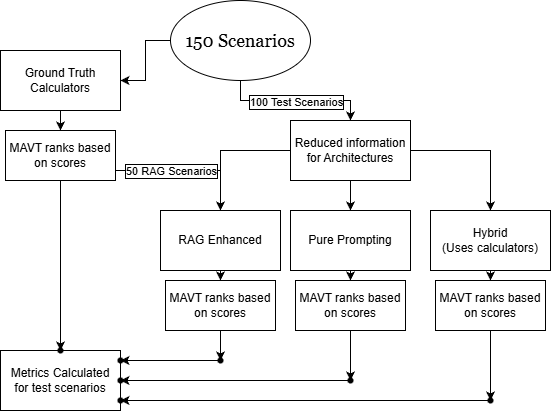
\includegraphics[width=0.5\textwidth]{FULLFlowMCDA.png}
  \caption{RAG and test scenarios do not overlap.}
\label{fig:full-flow-mcda}
\end{figure}
Figure~\ref{fig:full-flow-mcda} shows the full decision-support workflow common to all three architectures. The three architectures differ only in how the scoring step is performed.
\FloatBarrier

$\mathcal{A}_{\text{D}}$ and $\mathcal{A}_{\text{E}}$ both score one alternative at a time to prevent relative rather than absolute value ranking.

Failed outputs are marked with the number 1928--a reserved sentinel value and excluded from the main set of metrics--(Section~\ref{sec:eval-metrics}). However, an imputed set of metrics under an alternative failure-handling rule appear in Supplementary Material S2 to remove the advantage this would give models that failed more often.

Results are reported as five-run means $\pm$ standard deviations. Each architecture--model combination is run independently five times at temperature 0.3. Kendall's $\tau$, MAE, RMSE, and Top-1 accuracy are computed independently for each run, then averaged across the five runs. This per-run-then-average protocol measures the expected performance of a single deployment; the per-run standard deviation quantifies run-to-run stability: a low standard deviation means the architecture and model combination behaves consistently regardless of the random seed, which matters for production deployment where only one run is available. Supplementary Material S2 reports mean-aggregate consensus results.

Table~\ref{tab:parameter_comparison} details the parameters given to architectures vs.\ calculators, shown for HVAC as the illustrative case.
\begin{table*}[htpb]
\centering
\begin{threeparttable}
\footnotesize
\renewcommand{\arraystretch}{0.88}
\centering
\begin{tabular}{@{} l c c @{}}
\toprule
\textbf{Parameter} & \textbf{LLMs} & \textbf{Calc.} \\
\midrule
Location            & \checkmark & ---        \\
Outdoor Temp        & \checkmark & \checkmark \\
Home Size (sq ft)   & \checkmark & \checkmark \\
Insulation Tier$^{a}$   & \checkmark & ---        \\
R-Value             & ---        & \checkmark \\
Household Size      & \checkmark & \checkmark \\
Housing Type        & \checkmark & \checkmark \\
House Age$^{b}$     & \checkmark & \checkmark \\
Utility Budget      & \checkmark & \checkmark \\
SEER Rating         & ---        & \checkmark \\
Occupancy Context$^{c}$   & \checkmark & \checkmark \\
Indoor Temp (alt.)  & ---        & \checkmark \\
\bottomrule
\end{tabular}
\begin{tablenotes}
\footnotesize
\item[$a$] Given to the LLMs as a qualitative tier (Poor/Medium/Good); the calculator receives the corresponding numeric R-value.
\item[$b$] Given to the LLMs as a band label; recorded in the calculator's scenario record as raw years.
\item[$c$] Conveyed within the natural-language question text rather than as a separate field.
\end{tablenotes}
\end{threeparttable}
\caption{Scenario parameters available to LLM architectures vs.\ ground-truth calculators}
\label{tab:parameter_comparison}
\end{table*}
% NOTE: Appliance & Shower parameter tables could fit alongside this one.
\FloatBarrier

Appliance and Shower parameters follow the same visible/hidden split (full tables in Supplementary Material S1). The parameters given to the LLM architectures are chosen as they are parameters readily observable by a household occupant \cite{doehesscore2021}.


Each insulation tier spans a range of R-values drawn from standard U.S.\ residential wall assemblies \cite{cec_ja43_2013,energystar_insulation2023}: Poor scenarios use R-8 to R-12 (minimal 2$\times$4 cavity fill, below current code), Medium scenarios use R-13 to R-18 (standard 2$\times$4 batt through 2$\times$6 mixed), and Good scenarios use R-19 to R-24 (2$\times$6 framing and above). Consecutive tier midpoints differ by 55\% (R-10 to R-15.5) and 39\% (R-15.5 to R-21.5) in wall R-value. SEER ratings in the test corpus span 8--22, covering pre-1992 units (SEER~8--10), standard-efficiency replacements (SEER~13--14), and high-efficiency models (SEER~16--22), consistent with the ENERGY STAR Most Efficient threshold \cite{energystar_ac2023}.

The appliance age presented to the LLM architectures is a band label (1--3, 4--6, 7--9, 10--12, 13--17, and 28--32 years in the test corpus), derived from the scenario's raw integer age by a single shared helper so that the label is byte-identical on the query and index sides of retrieval. The band is a deliberately lossy proxy and is never an input to the physics: the scenario sheets retain both the raw age and an independent per-cycle energy value (kWh/cycle) drawn from the ENERGY STAR certified-products database, and the ground-truth calculator scores kWh/cycle directly without reference to age. Within a single appliance type the two are only moderately associated (Spearman's $\rho = 0.36$ for dishwashers, $0.38$ for dryers, and $0.69$ for washing machines), so two appliances sharing a band can differ materially in energy draw---a 7--9~year dryer ranges from 2.40 to 3.50\,kWh/cycle across the corpus. What the band withholds is precisely what the LLM architectures must infer. Housing type (apartment, condo, townhouse, rowhouse, twin, single-family) determines the envelope multiplier in the HVAC load equation and the noise propagation factor in the appliance comfort model; these mappings are detailed in Section~\ref{sec:gt-calculators}.

For the Flow Rate parameter, the scenario's numeric GPM is bucketed into three qualitative labels: \texttt{low\_flow} ($\le$2.0\,GPM, including EPA WaterSense certified showerheads \cite{epawatersense}), \texttt{standard} (2.5--3.0\,GPM, at or near the Energy Policy Act of 1992 federal maximum of 2.5\,GPM \cite{epawatersense}), and \texttt{high\_flow} ($>$3.0\,GPM). The label is present in the LLM test scenarios only, and is mapped from those ranges from the actual numeric GPM from the actual scenario.

The $\mathcal{A}_{\text{H}}$ architecture instead extrapolates these parameters from context before invoking the calculator (Section~\ref{sec:architectures}). The benchmark therefore measures whether $\mathcal{A}_{\text{H}}$ can bridge the gap between a fully specified reference calculator and the incomplete information a household could realistically provide.

\subsection{MAVT Framework \& Weighting Design}
\label{sec:mavt-design}
The Multi-Attribute Value Theory (MAVT) allows alternatives to be compared on different criteria based on the range of values that occurs for each criterion \cite{keeneyraiffa1976,dyer1979}.

The weights are held constant across all decision types, all architectures, and the ground-truth calculator. We did this so that any difference in score quality between decision types is because of the input accuracy and value function, not because of difference in the way each criterion weighted for the three decision types. Normally, MAVT additive form (Eq.~\ref{eq:mavt_sum}) requires preferential independence among criteria \cite{dyer1979,keeneyraiffa1976}. This means that criteria should be independent, meaning that the value (good or bad) of one criterion should have no effect on the value of another criterion.

\begin{equation}
\label{eq:mavt_sum}
s_j = \sum_{i=1}^{4} w_i \cdot v_i(x_{ij})
\end{equation}

In our dataset the energy cost and environmental impact criteria are not statistically independent: Spearman's $\rho$ between them is 0.92. This is not, however, a violation of the condition the additive form requires. Preferential independence is a property of the preference structure---that the rate at which the decision maker trades one criterion against another does not depend on the levels of the remaining criteria---and not a property of the empirical correlation between attribute values in a particular set of alternatives \cite{keeneyraiffa1976,dyer1979}. A household willing to accept a given increment of emissions for a given saving in cost at 20\,$^\circ$F would accept the same trade at 90\,$^\circ$F, so the additive form remains admissible at $\rho = 0.92$.

The correlation does, however, raise a distinct and legitimate concern---redundancy, or double counting---which arises if the two criteria are operationally the same quantity under different names, causing their combined 65\% weight to be applied twice to a single underlying attribute \cite{keeneyraiffa1976}. The extent to which this occurs differs sharply by decision type, and we state it explicitly rather than assume it away. Because ranking is performed within a scenario, the relevant quantity is the within-scenario association between the two criteria across the three alternatives.

For the Appliance decision type the two criteria genuinely separate. The price period is set by the utility's time-of-use window (for PECO, 2--6\,p.m.\ on weekdays \cite{peco2021}) while the emissions period is set by the PJM system-wide peak of 7\,a.m.--11\,p.m., so a cycle run at 8\,a.m.\ is off-peak for cost and on-peak for emissions. The magnitudes differ as sharply as the windows: moving from peak to off-peak cuts the PECO rate from \$0.320 to \$0.076/kWh, a 76\% reduction, but cuts marginal emissions only from 1.041 to 0.976\,lb\,CO\textsubscript{2}/kWh, a 6\% reduction. The within-scenario Spearman correlation between raw cost and raw emissions is defined in 50 of the 100 Appliance scenarios (in the other 50 at least one of the two quantities is constant across the three alternatives, so $\rho$ is undefined); over those 50 it averages 0.610, and 11 of them exceed 0.999.

For HVAC and Shower they do not separate. In both, the parameters that distinguish the emissions or water quantity from the cost quantity---the occupancy-resolved emissions factor for HVAC, the flow rate and heater setpoint for Shower---are scenario-level and therefore identical across the three alternatives, so within any one scenario the environmental quantity is a fixed scalar multiple of the cost quantity. The within-scenario Spearman correlation is 1.000 for 101 of the 105 HVAC scenarios (the four exceptions have a constant raw cost across the three alternatives, so $\rho$ is undefined) and for all 80 Shower scenarios, and after normalization the two criterion scores differ by a mean of only 0.006 (HVAC) and 0.053 (Shower) on the 0--1 scale. For these two decision types the four-criterion specification therefore operates as a three-criterion one, with an effective weight of 0.65 on a single cost/emissions dimension. This is a property of the specification we adopt, not a claim about households in general, and the benchmark should be read as evaluating the three architectures against that stated specification.

The realized influence of each criterion differs from its nominal weight because the three alternatives in a scenario span only a fraction of the global reference range. Table~\ref{tab:swing_weights} reports, for each criterion and decision type, the mean over scenarios of the nominal weight times the within-scenario score range, the quantity each criterion actually contributes to the spread in MAVT score within a choice set. Comfort at 0.20 out-swings energy cost and environmental impact combined at 0.65 for HVAC, and environmental impact at 0.35 has the smallest realized swing of any Appliance criterion.

\begin{table*}[htbp]
\centering
\begin{threeparttable}
\footnotesize
\centering
\renewcommand{\arraystretch}{1.15}
\begin{tabular}{lcccc}
\toprule
Criterion & Nominal Weight & HVAC & Appliance & Shower \\
\midrule
Energy Cost & 0.30 & 0.027 & 0.066 & 0.108 \\
Environmental Impact & 0.35 & 0.032 & 0.008 & 0.128 \\
Comfort & 0.20 & 0.086 & 0.098 & 0.069 \\
Practicality & 0.15 & 0.015 & 0.095 & 0.053 \\
\bottomrule
\end{tabular}
\renewcommand{\arraystretch}{1.0}
\end{threeparttable}
\caption{Mean within-scenario swing (nominal weight $\times$ within-scenario score range) by criterion and decision type.}
\label{tab:swing_weights}
\end{table*}

In our study, the benchmark harness uses the following weight configuration: Environmental Impact (35\%), Energy Cost (30\%), Comfort (20\%), and Practicality (15\%), as summarized in Table~\ref{tab:item3}. The vector is an input held constant across architectures and decision types so that the comparison is controlled, and results are reported across multiple weight configurations, including the baseline, equal weights, and the entropy- and MEREC-derived objective weight vectors in the weight robustness appendix (Appendix~\ref{app:weights}).

\begin{table*}[htbp]
\centering
\begin{threeparttable}
\footnotesize
\centering
\renewcommand{\arraystretch}{1.15}
\begin{tabular}{lllll}
\toprule
Criterion & Weight (\%) & Value Function & $\alpha$ & Direction \\
\midrule
Environmental Impact & 35 & Linear (Eq.~\ref{eq:linear_vf}) & \textemdash & Lower raw = better \\
Energy Cost & 30 & Linear (Eq.~\ref{eq:linear_vf}) & \textemdash & Lower raw = better \\
Comfort & 20 & Logarithmic (Eq.~\ref{eq:log_vf}) & 1.5 & Higher raw = better \\
Practicality & 15 & Logarithmic (Eq.~\ref{eq:log_vf}) & 1.2 & Higher raw = better \\
\bottomrule
\end{tabular}
\renewcommand{\arraystretch}{1.0}
\end{threeparttable}
\caption{MAVT criterion specification.}
\label{tab:item3}
\end{table*}

The Environmental Impact weight of 0.35 was assigned for two reasons. Residential emissions account for a sizable share of national CO\textsubscript{2} emissions \cite{dietz2009}, so a household decision-support tool that does not give priority to environmental impact fails in its objective. The Value--belief--norm theory, which says that environmental orientation is the most consistent normative driver across pro-environmental household behaviours, also applies heavily due to the nature of the people using the tool. \cite{stern1999,steg2005}. Finally, entropy-based normalization of the scenario distributions assigns higher information weight to the environmental criterion, which is consistent with an above-average allocation \cite{roszkowska2026}. These weights are computed on post-value-function scores, which depend on the reference ranges, the $\alpha$ values, and the budget penalty; they are therefore not independent of the design, and dispersion-based weights are descriptive rather than normative (see ~\ref{app:weights} for the full computation).

 Weighting Energy Cost at 0.30 keeps it slightly below environmental impact while keeping its role as the criterion households actually act on; for the average person, cost is the strongest predictor of consumer adoption. In fact, cost savings as shown on energy labels for consumer products were even more effective than actual energy cost and carbon emissions \cite{newell2014}. For HVAC decisions, thermostat setpoints determine electricity draw at the billing rate, and households respond by reducing the difference from outside temperature whenever they can \cite{managementscience_pricing2023}. For appliance decisions, energy cost depends on the time-of-use rate at which the appliance runs; a dishwasher shifted from peak to off-peak can cut its per-cycle cost by 49--76\% across the five time-of-use utilities modelled, making cost the criterion most responsive to scheduling changes. For shower decisions, water heating accounts for a significant share of residential energy costs and the per-shower increment is rarely visible to users, amplifying the underestimation bias found by Attari et al. and making cost-feedback interventions similarly effective. \cite{attari2010,reu2016,harrispoll2024}.

Comfort is weighted at 0.20. Thermal comfort is the second driver of HVAC behavior \cite{aqilah2022,karjalainen2007}. The set points used for HVAC comfort were based mainly off of ASHRAE 55 \cite{ashrae55_2020,fanger1970,vanhoof2008}. For appliance decisions, comfort is primarily a function of run-time delay: the calculator assumes, informed by demand-response acceptance research, that household willingness to accept a shift decays sharply beyond two to four hours, with dishwashers tolerated longest and dryers shortest \cite{paetz2012,waseem2020}, and the penalty scales further with household size as dishes and laundry accumulate faster. For shower decisions, comfort peaks around the REU2016 average of 7.8\,minutes \cite{reu2016,harrispoll2024} and depends additionally on temperature adequacy, with heater setpoints below CDC Legionella thresholds carrying a comfort penalty \cite{cdc2026}.

Practicality is weighted at 0.15. In our context, practicality means the likelihood that an activity will be continued long term. While this is partially linked to the other criterion, it also requires that the tool adds minimum friction relative to the existing routine. Otherwise, adoption of the tool drops \cite{ariely2001,leclerc1995,gardner2020,mergelsberg2020}. The lower weight (relative to comfort) is due to the fact that most of the decisions recommended by the tool are not likely to be repeated long-term or followed exactly. Additionally, practicality is a constraint on what is reasonable rather than a true user preference. Where comfort captures what a household would prefer given no constraints, practicality captures what is feasible and sustainable to adopt. A 15-minute shower may score near-optimally on comfort, but if four occupants share a 40-gallon tank, available hot water runs out before the third person showers. Practicality penalizes rather than eliminates such infeasible options: the 3.0 capacity penalty on the 0--10 scale contributes 0.043 of the 1.0-scale MAVT score, against a mean within-scenario cost-plus-environmental swing of 0.236 for Shower, so an infeasible alternative can still outrank a feasible one.

By requiring a score or parameter estimate for each of the four criteria, the structured framework prevents the LLM from arbitrarily selecting an alternative based on a single dominant attribute, a known failure mode of unaided LLM judgment \cite{wang2024fairescalers}.

Each criterion's raw quantity is first converted to a direction-adjusted normalized value $\tilde{x}$, so that higher values are always better:
\begin{equation}
\label{eq:norm_x}
\tilde{x} =
\begin{cases}
\dfrac{x - x_{\min}}{x_{\max} - x_{\min}} & \text{for increasing criteria}\\[2mm]
\dfrac{x_{\max} - x}{x_{\max} - x_{\min}} & \text{for decreasing criteria}
\end{cases}
\end{equation}

\begin{equation}
\label{eq:linear_vf}
v_i(\tilde{x}) = \tilde{x}
\end{equation}

The environmental and energy cost functions use the linear value function (Eq.~\ref{eq:linear_vf}) because equal absolute changes in these quantities represent equal improvements: a 1\,lb\,CO\textsubscript{2} reduction is equally valuable regardless of the baseline, and a \$0.10 saving carries the same decision weight at any cost level relative to the household's budget range \cite{dyer1979,keeneyraiffa1976}. Framing environmental impact in absolute physical units (lbs\,CO\textsubscript{2}) makes a linear preference the conservative modeling choice that treats identical emission reductions as equally desirable \cite{keeneyraiffa1976}.

\begin{equation}
\label{eq:log_vf}
v_i(\tilde{x}) = \frac{\ln\!\left(1 + \alpha \cdot \tilde{x}\right)}{\ln(1 + \alpha)}
\end{equation}

The comfort and practicality criteria use the logarithmic value function (Eq.~\ref{eq:log_vf}) because both exhibit diminishing marginal returns: initial improvements from an uncomfortable or impractical baseline yield disproportionately large perceived gains, while incremental improvements near the optimum matter progressively less. For comfort, moving from a temperature far outside the ASHRAE~55 band toward the neutral setpoint produces large subjective gains, but further refinement within an already acceptable range has little additional effect \cite{ashrae55_2020,fanger1970,vanhoof2008}. For practicality, adopting a behavior that fits within budget and routine constraints is a large step; further reducing friction beyond an already feasible option adds minimal value \cite{ariely2001,leclerc1995}. The shape parameter $\alpha = 1.5$ for comfort and $\alpha = 1.2$ for practicality were set a priori to introduce mild concavity; no elicitation was performed (e.g., midvalue splitting), and the values are not derived from data. Moderate gains (e.g., moving from the 25th to the 50th percentile of the criterion range) receive meaningful credit without over-rewarding marginal further improvements, while keeping the function close enough to linear that the difference in weights---rather than curvature---remains the dominant driver of the final MAVT score. Section~\ref{sec:res-sensitivity} reports the architecture ordering under all four $\alpha$ values; $\mathcal{A}_{\text{H}} > \mathcal{A}_{\text{E}} > \mathcal{A}_{\text{D}}$ is invariant across $\alpha \in \{1.0, 1.2, 1.5, 2.0\}$.

\subsection{Reference Ranges}

The reference ranges in Table~\ref{table:reference_ranges} are computed as the 5th--95th percentiles of the ground-truth cost distributions over the scenario corpus, and of the water-volume distribution for Shower, rather than extreme theoretical limits, so that normalization preserves meaningful spread across typical residential alternatives. The HVAC and Appliance environmental bounds are derived from the corresponding cost-per-kWh percentile envelope through the PJM marginal emission factors, as detailed below; the comfort and practicality bounds are constructed score bounds (0.0--1.0 and 0.05--1.0), not percentiles. However, since these values were used based on actual setpoints from Pennsylvania, they do reflect real world usage. Using dataset percentiles rather than the full theoretical physics envelope is a deliberate modeling choice \cite{roszkowska2026} at the cost of truncating scores for extreme outlier scenarios. The endpoints below are reported to two decimals.

\begin{table}[H]
\begin{threeparttable}
\centering
\small
\caption{Reference ranges (5th--95th percentiles for the cost quantities and Shower water volume; HVAC and Appliance environmental bounds derived from the cost envelope through the marginal emission factors; comfort and practicality are constructed score bounds). Shower Environmental Impact is reported in gallons of water; HVAC and Appliance in lbs CO\textsubscript{2}.}
\label{table:reference_ranges}
\begin{tabular}{@{}lccc@{}}
\toprule
\textbf{Criterion} & \textbf{HVAC} & \textbf{Appliance} & \textbf{Shower} \\
\midrule
Energy Cost (\$) & 0.38--3.29 & 0.025--0.71 & 0.14--1.14 \\
Environmental Impact & 1.96--18.04 & 0.288--3.643 & 6.0--45.0 \\
Comfort & 0.0--1.0 & 0.0--1.0 & 0.0--1.0 \\
Practicality & 0.05--1.0 & 0.05--1.0 & 0.05--1.0 \\
\bottomrule
\end{tabular}
\end{threeparttable}
\end{table}

For HVAC, cost percentiles reflect active-conditioning alternatives. A setpoint near outdoor temperature produces zero decision-period load and collapses to \$0, which makes the lower bound go to zero. The cost is estimated at \$0.19/kWh, which represents a bundled retail rate combining generation, transmission, distribution, monthly service fees, riders, and state taxes. Form EIA-861 reports a 2024 Pennsylvania statewide average price of 17.77\textcent/kWh based on total utility revenue divided by sales \cite{eia_epa_2024}. However, in urban and suburban Philadelphia, the Pennsylvania Public Utility Commission 2025 Rate Report lists an average monthly PECO residential bill of \$135.29 for 702\,kWh, establishing an effective bundled price of 19.27\textcent/kWh \cite{paupc2025}. Approved PUC rate settlements increase representative 700\,kWh PECO bills to \$149.43 in 2025 (21.3\textcent/kWh) and \$152.13 in 2026 (21.7\textcent/kWh) \cite{paupc2024dec}. The \$0.19/kWh baseline provides a conservative, empirical rate for Pennsylvania decision modeling. Excluding zero-load points, the realized 8-hour cost distribution at Pennsylvania's bundled residential rate (\$0.19/kWh) \cite{eia_epa_2024,paupc2025,paupc2024dec} spans \$0.38--\$3.29.  An Off option receives top cost score via decreasing-value normalization. These endpoints match residential HVAC efficiency benchmarks \cite{synapse2013,parker2018,huyen2019}.

Using this kWh distribution with PJM marginal emissions factors (0.976 off-peak, 1.041 peak lbs CO\textsubscript{2}/kWh) yields HVAC environmental bounds of 1.96--18.04 lbs CO\textsubscript{2} \cite{pjm2022emissions}.


For appliances, the realized per-cycle cost distribution (kWh/cycle multiplied by the resolved time-of-use rate across the six PA utilities) spans \$0.025--\$0.71, and the realized per-cycle emissions distribution (kWh/cycle through the PJM marginal factor at run time) spans 0.288--3.643 lbs CO\textsubscript{2}. The underlying per-cycle energy endpoints remain consistent with the ENERGY STAR certified-products distribution (efficient HE washers near 0.25\,kWh) and include the older non-certified electric resistance dryers \cite{energystar_products,chenyu2018,hustvedt2013,neep2015,porras2020}.

For showers, the realized per-shower cost distribution spans \$0.14--\$1.14. Shower energy follows the mixing-fraction physics targeting a fixed 105\,\textdegree{}F delivery temperature, so it depends only on the rise from the mains inlet (seasonal inlet temperatures from NREL hot-water modeling \cite{hendron2008}) to that target and is independent of heater setpoint for setpoints at or above the 105\,\textdegree{}F delivery target, which all corpus setpoints (105--140\,\textdegree{}F) satisfy; cost is this energy priced at the PA residential rate. 

Shower environmental impact is defined as water volume (gallons); the realized distribution of flow rate multiplied by duration spans 6.0--45.0 gallons at the 5th--95th percentile, with flow-rate and duration benchmarks from EPA WaterSense Appendix~B \cite{epawatersense}, REU2016 \cite{reu2016}, and The Harris Poll \cite{harrispoll2024}. Water volume is the household-salient environmental externality of showering, and showers account for a major share of indoor residential water use. 

\subsection{Ground Truth Calculators}
\label{sec:gt-calculators}
Each ground-truth calculator consumes a scenario with three alternatives and returns four scores per alternative---Energy Cost (\$), Environmental Impact, Comfort, and Practicality---plus the raw physical quantities for environmental impact and energy cost before value-function transformation. Energy cost is in dollars per 8-hour decision period (HVAC), per cycle (Appliance), or per shower (Shower); monthly estimates are computed only for the budget penalty; Environmental Impact is in lbs\,CO\textsubscript{2} for HVAC and Appliance decisions and in gallons of water for Shower decisions.

For HVAC and Appliance decisions, environmental impact uses PJM marginal emissions factors:
\begin{equation}
\begin{split}
  \mathrm{CO_2} &= E_{\mathrm{kWh}} \cdot \varepsilon(t), \\
  \varepsilon(t) &= \begin{cases}
    1.041 \text{ lbs/kWh} & \text{peak (7am--11pm)} \\
    0.976 \text{ lbs/kWh} & \text{off-peak}
  \end{cases}
\end{split}
  \label{eq:emissions}
\end{equation}
\noindent where $E_{\mathrm{kWh}}$ is the decision-period energy use and $\varepsilon(t)$ is the PJM marginal emissions factor at run time $t$ \cite{pjm2022emissions}. Marginal rather than average factors are used because shifting a residential load displaces or adds the generator at the margin.
All three calculators apply an identical four-tier budget penalty $P(u)$ multiplicatively to the energy-cost value-function output, where $u = C_{\mathrm{monthly}} / B$ is monthly cost utilization relative to the household's stated budget $B$:
\begin{equation}
  P(u) = \begin{cases}
    1.0                          & u < 0.80                   \\[4pt]
    1 - 2.5\,(u - 0.80)         & 0.80 \le u < 1.0           \\[4pt]
    0.5\,e^{-3(u - 1.0)}        & 1.0 \phantom{0}\le u < 1.5 \\[4pt]
    0                            & u \ge 1.5
  \end{cases}
  \label{eq:budget_penalty}
\end{equation}
\noindent where $P(u)$ is a unitless multiplicative penalty on the (post value-function) energy-cost score, $u$ is monthly budget utilization, $C_{\mathrm{monthly}}$ is estimated monthly energy/water-related cost for the decision type, $B$ is the household-stated monthly budget for utilities, and $e$ is Euler's number.
\noindent The no-penalty zone ($u < 0.80$) reflects mental budget safety margins \cite{thaler1999}; the linear decline approaching the limit follows \cite{heath1996}'s budget self-control model; exponential loss aversion for overruns follows \cite{prelec1998} and \cite{heutel2017}; and elimination beyond 150\% reflects financial infeasibility \cite{gathergood2012}. Applying the penalty multiplicatively ensures extremely cheap or expensive alternatives cannot completely sway ranking on energy cost alone.

\noindent For HVAC decisions, $C_{\mathrm{monthly}} = 90\,C_{\mathrm{8h}}$, where $C_{\mathrm{8h}}$ is the energy cost for one 8-hour conditioning period and 90 is three such periods per day across 30 days. The Appliance and Shower monthly-cost conversions are given in Eq.~\ref{eq:appliance_monthly_cost} and Eq.~\ref{eq:shower_monthly_cost}.

\subsubsection{HVAC Calculator}
Thermal load decomposes into four ASHRAE-style components. For cooling:
\begin{equation}
\begin{split}
  Q_{\mathrm{cool}} ={} &
    \underbrace{\frac{m \cdot A}{R}\,\Delta T}_{\text{conductive}}
    +\underbrace{400n + A + 800}_{\text{internal}} \\
    &+\underbrace{0.15\,A \times 20}_{\text{solar}}
    +\underbrace{1.08\,\frac{A\, h_c\, \alpha}{60}\,\Delta T}_{\text{infiltration}}
\end{split}
  \label{eq:hvac_cooling_load}
\end{equation}
\noindent where $A$ is floor area (sq\,ft); $m$ is a housing-type envelope multiplier (1.7 single-family, 1.6 twin/semi-detached, 1.5 townhouse/rowhouse, 1.2 apartment/condo), a modeling assumption of the calculator \cite{accamanualj}; $R$ is the wall insulation R-value; $\Delta T = T_{\mathrm{out}} - T_{\mathrm{in}}$; $n$ is household size; $h_c = 8$\,ft and $\alpha = 0.35$\,ACH for ceiling height and infiltration rate \cite{polly2011,ashrae62_1_1989}. The 800\,BTU/hr baseline captures always-on standby loads per the ASHRAE Handbook of Fundamentals (Chapter~18, Table~1) \cite{ashrae_hof2017}. The heating load uses the same expression with $\Delta T = T_{\mathrm{in}} - T_{\mathrm{out}}$, no solar term, and internal gains subtracted rather than added.

Effective EER is estimated from the unit's rated SEER via a quadratic approximation \cite{ahri2008}, a modeling assumption of the calculator:
\begin{equation}
  \mathrm{EER} = -0.02\,\mathrm{SEER}^{2} + 1.12\,\mathrm{SEER}
  \label{eq:eer_quadratic}
\end{equation}
\noindent where $\mathrm{SEER}$ is the unit's rated seasonal energy efficiency ratio and $\mathrm{EER}$ is the resulting effective energy efficiency ratio used for the decision period. Age- and maintenance-driven efficiency degradation is deliberately \emph{not} applied to the energy path; it is instead modeled as a reliability factor in the practicality score (Eq.~\ref{eq:hvac_degradation}), so the energy score reflects the setpoint choice rather than the system's condition. The practicality score is scaled by $(1 - D)$, where
\begin{equation}
  D = \min\!\Bigl(0.30,\; \delta_{\mathrm{maint}}\bigl[\,1.5\min(a,10) + 0.5\max(a-10,0)\,\bigr]\Bigr)
  \label{eq:hvac_degradation}
\end{equation}
\noindent is the fraction of efficiency lost (capped at 30\%), $a$ is HVAC age in years, and $\delta_{\mathrm{maint}}$ is the base annual loss rate (0.005, 0.010, 0.015 per year for good, moderate, and poor upkeep); the first ten years degrade at $1.5\,\delta_{\mathrm{maint}}$ and later years at $0.5\,\delta_{\mathrm{maint}}$, a modeling assumption of the calculator \cite{domanski2014}; an intermediate floor of 0.5 (on the 0--10 scale) is applied to the practicality score before the $\Delta T$ and degradation multipliers, and the final score is clipped to $[0.15, 1.0]$. Energy consumption over the 8-hour decision window is then:
\begin{equation}
  E_{\mathrm{kWh}} =
    \frac{Q_{\mathrm{load}}}{\mathrm{EER} \times 1000}
    \cdot 8 \cdot m_{\mathrm{occ}}
  \label{eq:hvac_energy}
\end{equation}
\noindent where $Q_{\mathrm{load}}$ is the thermal load (BTU/hr) for the decision context and $m_{\mathrm{occ}}$ scales for occupancy context: 1.0 for fully occupied, 0.75 for overnight, and $1 - 0.5(h_{\mathrm{away}}/24)$ for daytime unoccupied periods \cite{houde2021}, where $h_{\mathrm{away}}$ is hours-away per 24-hour day.

Because HVAC alternatives carry no explicit run-time, the marginal emissions factor in Eq.~\ref{eq:emissions} is resolved from the occupancy context by applying each pattern onto the PJM peak (7am--11pm, 16\,h) and off-peak (8\,h) windows, with away-hours assumed to fill the daytime peak window first:
\begin{equation}
\footnotesize
  \varepsilon_{\mathrm{occ}} =
  \begin{cases}
    \varepsilon_{\mathrm{off}} & \text{occupied-sleep (night-only runtime)} \\[4pt]
    \dfrac{16\,\varepsilon_{\mathrm{pk}} + 8\,\varepsilon_{\mathrm{off}}}{24}
      & \text{occupied all day} \\[8pt]
    \varepsilon_{\mathrm{pk}} & \text{unoccupied } H\text{\,hr},\; H \le 16 \\[4pt]
    \dfrac{16\,\varepsilon_{\mathrm{pk}} + (H-16)\,\varepsilon_{\mathrm{off}}}{H}
      & \text{unoccupied } H\text{\,hr},\; H > 16
  \end{cases}
  \normalsize
  \label{eq:hvac_occ_emissions}
\end{equation}
\noindent where $\varepsilon_{\mathrm{pk}} = 1.041$ and $\varepsilon_{\mathrm{off}} = 0.976$\ (in terms of lbs/kWh) are the PJM peak and off-peak marginal factors and $H$ is hours-away per day \cite{pjm2022emissions}. Occupied-sleep returns the off-peak factor because the home's conditioning runtime falls entirely in the overnight off-peak window.

Comfort uses a tent function anchored to ASHRAE\,55 PMV-optimal setpoints \cite{ashrae55_2020,vanhoof2008,fanger1970}:
\begin{equation}
  C_{\mathrm{comfort}} = \tfrac{1}{10}\max\!\Bigl(0,\; 10 - \lvert T_{\mathrm{in}} - T^{*}\rvert - \tfrac{(n-3)\,0.3\,\lvert T_{\mathrm{in}} - T^{*}\rvert}{3}\Bigr)
  \label{eq:hvac_comfort}
\end{equation}
\noindent where $C_{\mathrm{comfort}}$ is a 0--1 comfort score, $T_{\mathrm{in}}$ is the indoor setpoint, $T^{*}$ is the context-dependent optimal setpoint used as the peak of the tent function ($76$\,\textdegree{}F in cooling mode, $70$\,\textdegree{}F in heating mode, consistent with ASHRAE\,55-2020 sedentary PMV bands \cite{ashrae55_2020}). The 76\,\textdegree{}F and 70\,\textdegree{}F optima are the midpoints of the ASHRAE\,55-2020 summer band (73--79\,\textdegree{}F at 0.5\,clo) and winter band (68--74\,\textdegree{}F at 1.0\,clo) for sedentary occupants, with the heating optimum 1\,\textdegree{}F below the 71\,\textdegree{}F winter midpoint. The $-1.0$ score-per-degree slope mirrors the rising PPD per degree outside neutrality in Fanger's PMV/PPD model \cite{fanger1970,vanhoof2008}. This PMV/PPD basis applies to mechanically conditioned spaces; the adaptive comfort model \cite{dedear2002} applies to naturally conditioned buildings and is not used. The penalty term applies only for household sizes $n > 3$, and $n$ is household size.
Practicality utility follows a piecewise value function of setpoint extremity, indoor--outdoor $\Delta T$, and equipment age. This is the first of five comfort and practicality utilities defined this way across the three calculators; full derivations for all of them are in Supplementary Material S1.

An ``Off'' alternative (no active conditioning) is scored with zero decision-period energy, cost, and emissions; its comfort and practicality are instead evaluated against the free-float indoor temperature the building drifts to with the system off --- outdoor $+5$\,\textdegree{}F in cooling season and $+10$\,\textdegree{}F in heating season, reflecting solar and internal gains that hold a closed, occupied house above outdoor air temperature \cite{ashrae55_2020,accamanualj,ashrae_hof2017}.

\subsubsection{Appliance Calculator}
Energy cost per cycle is

\begin{equation}
    C = E_{\mathrm{cyc}} \cdot r(t,\ell)
\end{equation}

where $E_{\mathrm{cyc}}$ is kWh/cycle and $r(t,\ell)$ is the location- and time-specific TOU rate resolved to one of six Pennsylvania utilities (PECO, PPL, West Penn, Penelec, MetEd, Duquesne) \cite{peco2021,ppl2025,firstenergy2025,firstenergy2026,duquesne2026} (see Supplementary Material S1 for the full rate structure).
\noindent. $C$ is per-cycle energy cost (dollars/cycle), $E_{\mathrm{cyc}}$ is per-cycle energy use (kWh/cycle), $t$ is the appliance run time (time-of-day), and $\ell$ is the household location used to resolve the serving utility.

The PJM emissions window (7am--11pm) applies to environmental impact regardless of the utility's billing window, because emissions follow the regional grid.
The run-time rate period is selected by mapping location $\ell$ to a utility $U(\ell)$ and then applying that utility's TOU peak window otherwise.
\begin{equation}
\begin{split}
(h^{U}_{\mathrm{pk,s}}, h^{U}_{\mathrm{pk,e}}):
\quad
r(t,\ell)&=r^{U}_{\mathrm{pk}}
\text{ if }
h(t)\in[h^{U}_{\mathrm{pk,s}}, h^{U}_{\mathrm{pk,e}}) \\
&\text{ and }
r(t,\ell)=r^{U}_{\mathrm{off}}
\end{split}
\end{equation}
\noindent where $U(\ell)$ maps location $\ell$ to a serving utility, $h^{U}_{\mathrm{pk,s}}$ and $h^{U}_{\mathrm{pk,e}}$ are that utility's TOU peak-window start and end hours, $r^{U}_{\mathrm{pk}}$ and $r^{U}_{\mathrm{off}}$ are the utility's peak and off-peak energy prices (\$/kWh), and $h(t)$ maps time $t$ to an hour-of-day on a 24-hour clock.
\noindent In the implementation, the six utilities use two distinct peak windows (2--6pm and 2--9pm). Duquesne is modelled with identical peak and off-peak rates (0.1375 \$/kWh), so scheduling does not affect the energy-cost criterion for its served scenarios: 11 of the 65 Appliance Test scenarios are Duquesne-served. The appliance calculator does not model weekend or holiday peak-hour pricing; all days use weekday TOU rates. Seasonal peak-window shifts are also unmodeled: PPL's winter (Dec--May) peak window is 4--8pm versus the 2--6pm summer window applied here; the summer window is used year-round because scenarios carry no season or date field. This simplification shifts the optimal scheduling window by 1--2 hours for some utilities in winter months.

Comfort utility is parameterized by delay, appliance type, housing type, household size, and run-time hour (late-night runs, 22:00--07:00, incur a noise penalty); practicality utility by delay, run-time hour, and household coordination difficulty (Supplementary Material S1).
For budget utilization in \eqref{eq:budget_penalty}, the appliance calculator converts per-cycle cost to a monthly estimate as:
\begin{equation}
  C_{\mathrm{monthly}} = c(\mathrm{type})\,C_{\mathrm{cycle}}, \qquad
  c(\mathrm{type})=
  \begin{cases}
    18 & \text{dishwasher} \\[2pt]
    25 & \text{washer} \\[2pt]
    24 & \text{dryer}
  \end{cases}
  \label{eq:appliance_monthly_cost}
\end{equation}
\noindent where $C_{\mathrm{cycle}}$ is per-cycle energy cost and $c(\mathrm{type})$ is the appliance-specific cycles-per-month estimate, from 215, 300, and 283 cycles/year for dishwashers, washers, and dryers respectively \cite{energystar_dishwasher_criteria2023,energystar_clotheswasher,doe_dryer_tp_2011}.

\subsubsection{Shower Calculator.}
Mains inlet temperature is interpolated from outdoor temperature between 45\,\textdegree{}F (winter, $T_{\mathrm{out}} \le 32$\,\textdegree{}F) and 65\,\textdegree{}F (summer, $T_{\mathrm{out}} \ge 75$\,\textdegree{}F) \cite{hendron2008,backman2013,maguire2013}. Only the fraction of flow requiring heating reaches the heater; that mixing fraction is:
\begin{equation}
  f_{\mathrm{hot}} = \frac{T_{\mathrm{target}} - T_{\mathrm{inlet}}}
                          {T_{\mathrm{heater}} - T_{\mathrm{inlet}}}
  \label{eq:shower_fraction}
\end{equation}
\noindent where $f_{\mathrm{hot}}$ is the fraction of total flow drawn as hot water, $T_{\mathrm{target}} = 105$\,\textdegree{}F is the standard comfortable delivery temperature \cite{zhang2023}, $T_{\mathrm{inlet}}$ is mains inlet temperature, and $T_{\mathrm{heater}}$ is the water-heater setpoint temperature. Shower energy is then:
\begin{equation}
  E_{\mathrm{kWh}} = \frac{\dot{V} \cdot f_{\mathrm{hot}} \cdot 8.33 \cdot
                            (T_{\mathrm{heater}} - T_{\mathrm{inlet}}) \cdot \tau}
                          {3412 \cdot \eta}
  \label{eq:shower_energy}
\end{equation}
\noindent where $E_{\mathrm{kWh}}$ is shower energy use (kWh), $\dot{V}$ is total flow rate (GPM), $\tau$ is shower duration (min), $\eta = 0.92$ is the unified energy factor for a 40--55\,gal electric tank \cite{rheem2025}, and $3412$\,BTU/kWh is the standard conversion; the constant $8.33$\,lb/gal converts gallons to pounds of water.

Environmental impact is water volume:
\begin{equation}
    V = \dot{V} \cdot \tau
    \label{eq:shower_volume}
\end{equation}
\noindent measured in gallons, where $\dot{V}$ is total flow rate (GPM) and $\tau$ is shower duration (min).

Energy cost uses a flat electricity rate $p_e$:
\begin{equation}
  C_{\$}=p_e\,E_{\mathrm{kWh}}.
  \label{eq:shower_cost}
\end{equation}
\noindent where $C_{\$}$ is shower energy cost (dollars) and $p_e$ is the electricity price (\$/kWh).
Comfort utility is parameterized by duration, heater setpoint, household contention, and outdoor temperature, which shifts the comfort-optimal duration upward in cold weather; practicality utility by duration and tank-capacity feasibility (Supplementary Material S1). The comfort-optimal duration follows the REU2016 7.8-minute average above 77\,\textdegree{}F and reaches about 10.3 minutes at the winter cap (10\% per 10.8\,\textdegree{}F drop); the calculator flags the elasticity as a modeling assumption rather than a directly reported coefficient and the cap as a cross-population extrapolation from a southern-Spain sample.
For budget utilization in the budget penalty equation, shower monthly cost is estimated from per-shower cost using an average showers-per-person-per-day rate:
\begin{equation}
  C_{\mathrm{monthly}} = C_{\mathrm{shower}} \cdot \bigl(n \cdot 0.9 \cdot 30\bigr).
  \label{eq:shower_monthly_cost}
\end{equation}
\noindent where $C_{\mathrm{shower}}$ is per-shower energy cost, $n$ is occupants, $0.9$ is showers/person/day \cite{reu2016}, and $30$ is days/month.

\noindent The anchor points that set the band boundaries are sourced (the 7.8-minute REU2016 average, the 15-minute Harris Poll threshold, the CDC Legionella range, and the ASHRAE\,55 comfort band \cite{reu2016,harrispoll2024,cdc2026,ashrae55_2020}), while the penalty magnitudes and slopes between those boundaries (the 3.0 capacity penalty, the 0.5 per-minute contention penalty, the 0.80 usable-tank fraction, and the piecewise practicality slopes) are design choices with no literature source.

\subsection{Architecture Implementations}
\label{sec:architectures}
All three architectures call the same model per test via OpenRouter at temperature 0.3, a moderate value that balances instruction-following fidelity against output diversity, with model held constant within each run.
At temperature 0 the five runs would be identical, collapsing the repeated-measures design to a single sample and leaving run-to-run variance unestimable; 0.3 preserves enough sampling variation for the five-run averaging and the reported variance to be meaningful. Temperature was not ablated in this study; the choice is a design constraint of the repeated-measures protocol rather than an empirically tuned value. The study evaluates four models spanning a range of capability, reasoning support, and cost: GPT-OSS-20B (\texttt{openai/gpt-oss-20b:exacto}, reasoning, low effort), Qwen 3.5 9B (\texttt{qwen/qwen3.5-9b:exacto}, non-reasoning), DeepSeek V4 Flash (\texttt{deepseek/deepseek-v4-flash:exacto}, hybrid reasoning), and Gemini 3.5 Flash (\texttt{google/gemini-3.5-flash:exacto}, reasoning, minimal effort). The \texttt{:exacto} suffix is an OpenRouter provider-routing variant that restricts serving to providers meeting a fixed accuracy standard; it is part of the model identifier and is required to reproduce these runs. Each was set to its lowest possible reasoning tier. Alternative order in the prompt was fixed (alt-1, alt-2, alt-3 in scenario-sheet order) across all runs and was not randomized. Ties in the MAVT aggregate were broken deterministically by the priority order environmental, energy cost, comfort, practicality. The rule fires often enough to disclose, because $\mathcal{A}_{\text{D}}$ and $\mathcal{A}_{\text{E}}$ scores come from the LLM on a coarse grid. At least two alternatives share a weighted score in 3.2\% of Gemini's $\mathcal{A}_{\text{D}}$ scenarios, 5.9\% of DeepSeek's, 12.6\% of GPT-OSS's and 21.3\% of Qwen's, and in 2.7\%, 19.1\%, 6.4\% and 13.9\% of the same four models' $\mathcal{A}_{\text{E}}$ scenarios. All three alternatives carrying identical scores on all four criteria is rarer, between 0.0\% and 1.2\% in every model--architecture cell, so the rule usually separates alternatives that already differ on at least one criterion.

\begin{figure}[H]
	\centering
	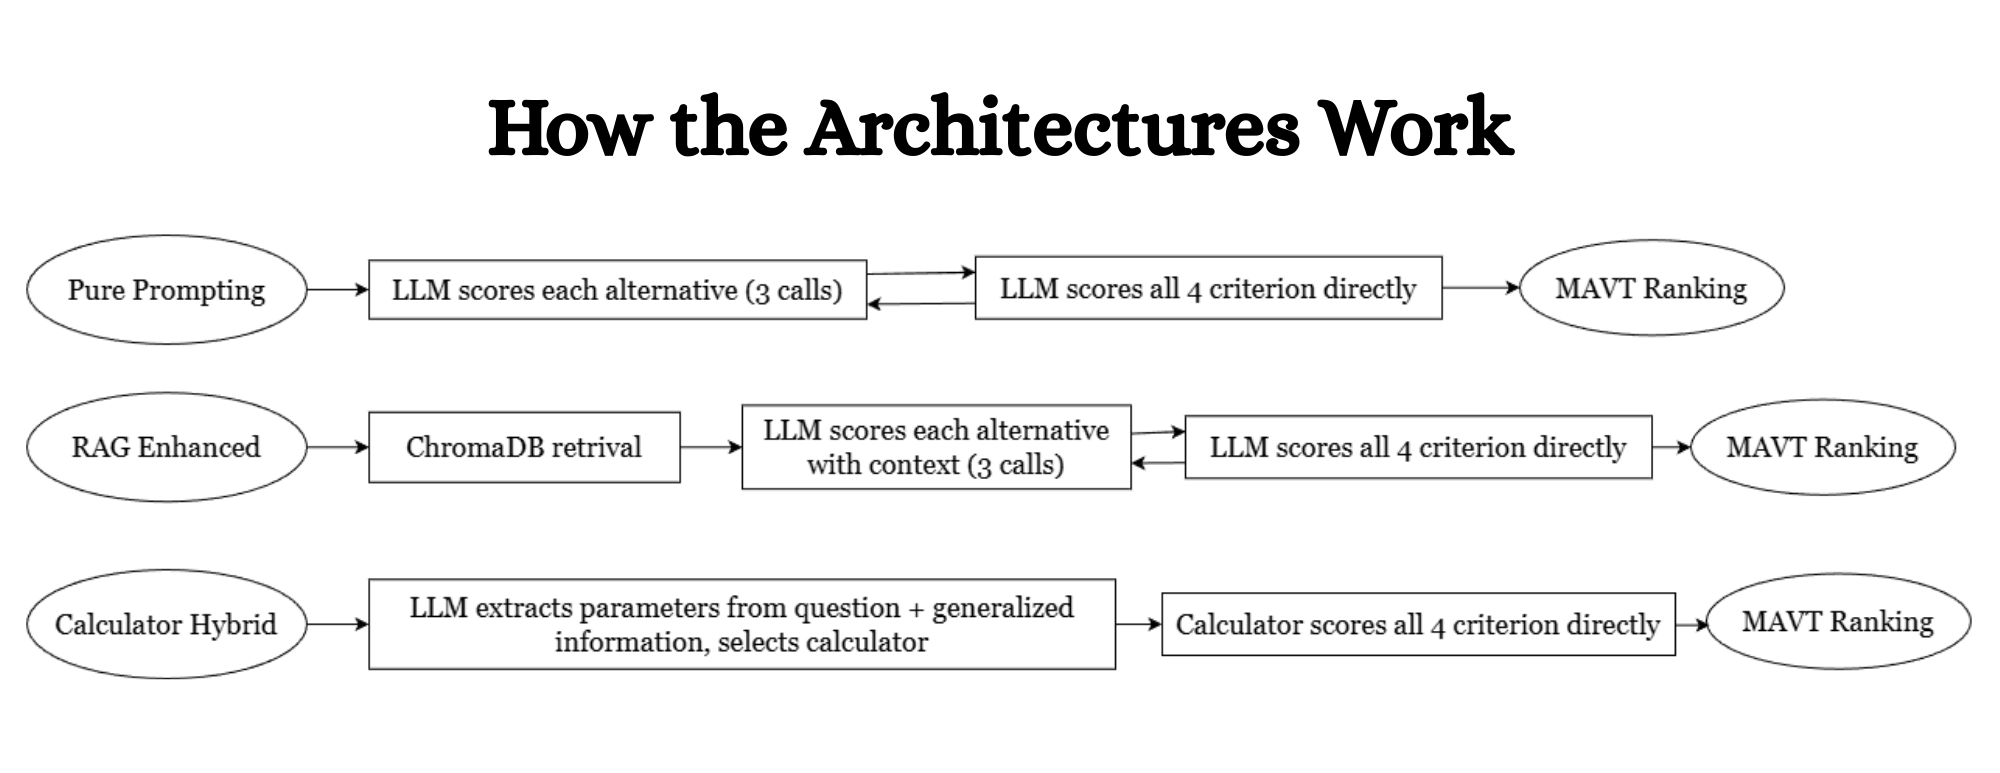
\includegraphics[width=1\textwidth]{ArchitectureFlowcharts.png}
  \caption{Processing pipeline for each architecture.}
\label{fig:pipeline}
\end{figure}

Figure~\ref{fig:pipeline} shows the processing pipeline for each architecture; the three architecture implementations are described below.



\subsubsection{\texorpdfstring{$\mathcal{A}_{\text{D}}$}{A_D} (Direct Prompting)}
The $\mathcal{A}_{\text{D}}$ architecture issues one API call per alternative (three calls per scenario) using a calibrated system prompt that combines role-prompting \cite{shanahan2023}, structured-output constraints \cite{wei2022cot}, and explicit bias-mitigation language drawn from the NIST framework for identifying and managing AI bias \cite{nistsp1270}. No external context is supplied beyond the scenario description. The system prompt establishes the analyst role and, for each of the three decision types, gives each of the four criteria a short anchor phrase describing what a good and a poor score look like on that criterion. It closes with a strict JSON-only output instruction and a reminder to distinguish between criteria, consistent with the bias-mitigation language cited above (full prompt text in Supplementary Material S1).

\noindent The user prompt provides the scenario context and asks the model to score one alternative at a time, including the other alternatives as reference so that it doesn't assign the same scores to all alternatives. 

The anchors are deliberately qualitative rather than numeric. For HVAC and Shower, each criterion is described by a good/moderate/poor triple stated in terms of the physical situation (for HVAC energy cost, ``good when the setpoint demands little from the system given outdoor conditions \ldots\ poor when the setpoint requires extreme effort''), with no numeric thresholds, units, or example values attached. The Appliance anchors reference the off-peak and peak rate periods and the overnight minimum of the grid-emissions profile, coarser domain information than the HVAC and Shower anchors carry, and the $\mathcal{A}_{\text{E}}$ prompt omits these lines, so on Appliance $\mathcal{A}_{\text{D}}$ receives the diurnal structure of the rate and emissions schedules that $\mathcal{A}_{\text{E}}$ must recover from a single retrieved exemplar. Supplying anchors would leak the calculator's reference ranges (Table~\ref{table:reference_ranges}) into the prompt and convert the task from judgment into interpolation; supplying no anchors at all leaves the 0--1 scale undefined, which is the condition under which LLM scorers exhibit the strongest scoring bias and compress their outputs into a narrow band \cite{li2026scoringbias,nistsp1270}. The verbal triple fixes the direction and the endpoints of each scale without fixing its calibration. Neither prompt states any Pennsylvania-specific quantity: $\mathcal{A}_{\text{D}}$ is given the location and must supply the PECO time-of-use tiers and the PJM marginal emissions factors from its own knowledge, whereas $\mathcal{A}_{\text{E}}$'s retrieved exemplar is a worked Pennsylvania case with reference scores attached. Part of the $\mathcal{A}_{\text{D}}$--$\mathcal{A}_{\text{E}}$ gap is therefore access to locale-specific values rather than scoring ability alone.

As a concrete instance, for the HVAC scenario ``I'm working from home today with 1 person, what AC temperature should I set?'' (Lancaster, PA; 92\,$^\circ$F outdoor; 1050\,sq\,ft; Good insulation; apartment, 21--30 years old; \$160/month budget), $\mathcal{A}_{\text{D}}$ is called once for each of the three setpoints 72, 76, and 80\,$^\circ$F. On the 76\,$^\circ$F call the model returns \texttt{\{"energy\_cost": 0.75, "environmental": 0.75, "comfort": 0.60, "practicality": 0.80\}}, which Eq.~\ref{eq:mavt_sum} aggregates to $0.30(0.75)+0.35(0.75)+0.20(0.60)+0.15(0.80)=0.728$. The same procedure applied to the other two setpoints yields the architecture's ranking for the scenario; no calculator is involved at any point.

\subsubsection{\texorpdfstring{$\mathcal{A}_{\text{E}}$}{A_E} (Example-Guided LLM Scoring)}
The $\mathcal{A}_{\text{E}}$ architecture retrieves the single most similar scenario ($k=1$) from a ChromaDB vector store before scoring, using the sentence-transformers/all-MiniLM-L6-v2 embedding model. The retrieval count $k=1$ was selected based on a development-set ablation (Section~\ref{sec:rag-ablation-methods}): no retrieval count differed detectably at the power available in three of the four models, whose percentile bootstrap 95\% CIs on the $k{=}1$ minus $k{=}3$ Kendall's $\tau$ difference all contain zero (Gemini $[-0.163, 0.142]$, GPT-OSS $[-0.128, 0.228]$, Qwen $[-0.047, 0.326]$), although DeepSeek's $k{=}1$ mean $\tau$ sits 0.316 below its $k{=}3$ mean with CI $[-0.471, -0.161]$; so $k=1$ was chosen as the production setting to minimize token and API cost as the cheapest configuration not shown to be worse (full ablation results in Section~\ref{sec:rag-ablation}).

Measured over the full 195-scenario test set, the L2 distance between the unnormalized all-MiniLM-L6-v2 embeddings of each Test scenario and its nearest same-type corpus entry ranges from 0.066 to 0.427 (median 0.215, mean 0.221), with nearest-neighbour medians of 0.249 for HVAC, 0.207 for Appliance, and 0.164 for Shower. A uniformly random same-type corpus entry sits at a mean L2 distance of 0.422, roughly twice the nearest-neighbour median, so the coverage claim rests on this measurement rather than on the corpus design.

The retrieved exemplar is rendered as a full worked example: its household-reported parameters, its engineering parameters (R-value, SEER, GPM, kWh/cycle, tank size, heater setpoint, etc.), and each of its alternatives with the four ground-truth criterion scores plus the MAVT aggregate and rank. The exemplar's engineering values are shown so the model can see how those values map to scores. The model is instructed to use the exemplar as reference but to score the target scenario independently. Like $\mathcal{A}_{\text{D}}$, $\mathcal{A}_{\text{E}}$ uses three API calls per scenario (one per alternative). The retrieval index is built once from the 90 RAG-only scenarios described in Section~3.1; test scenarios are used only as query vectors and the index stores only RAG scenarios \cite{lewis2020}.

The system prompt keeps $\mathcal{A}_{\text{D}}$'s analyst role, JSON-only output format, and criteria-distinction instruction, but replaces the twelve per-decision-type anchor descriptions with four one-line statements of each criterion's direction (lower cost, lower emissions, higher comfort, easier implementation), since the RAG exemplars supply scoring guidance in the anchors' place. The $\mathcal{A}_{\text{D}}$--$\mathcal{A}_{\text{E}}$ contrast therefore varies criterion framing alongside retrieval and is not a clean isolation of retrieval alone; the \texttt{no\_anchors} prompt ablation (Section~\ref{sec:prompt-ablation-methods}) bounds the anchor component of that difference (full prompt text in Supplementary Material S1).


\noindent The user prompt presents the target scenario, the alternative to score, and the retrieved exemplar---with household-reported parameters, engineering values, and the four ground-truth scores plus MAVT aggregate and rank---instructing the model to ``consider how this specific alternative performs given the scenario context.'' 

\subsubsection{\texorpdfstring{$\mathcal{A}_{\text{H}}$}{A_H} (LLM-Parameterized Reference Scoring)}
The $\mathcal{A}_{\text{H}}$ architecture issues a single API call per scenario for structured parameter extraction. Known household-reported scenario fields (outdoor temperature, square footage, insulation tier, household size, housing type, utility budget, and location) are passed directly to the calculator without LLM involvement, and the three alternatives are taken verbatim from the scenario sheet---the deterministic calculator, not the LLM, parses the numeric content of each alternative string (setpoint temperature, run time, or shower duration). The LLM is asked only to estimate the genuinely withheld engineering parameters that are absent from the household-reported description: for HVAC, the wall R-value, SEER rating, and HVAC age, with the occupancy context read from the question text rather than withheld; for Appliance, the kWh/cycle, with the appliance type and current baseline time also stated in the question; for Shower, the numeric GPM (estimated from the household-reported flow-rate label), tank size, and water-heater setpoint.

The extracted JSON is validated before execution. A validation script checks extracted parameters against physical limits: HVAC wall R-value (1.0--60.0), SEER (6.0--30.0), equipment age (0.0--60.0 years); appliance energy (0.05--10.0 kWh/cycle); and shower flow rate (0.5--8.0 GPM), tank capacity (10.0--120.0 gallons), and water heater setpoint (80.0--160.0\,$^\circ\text{F}$). If an LLM predicts an out-of-range value or returns non-numeric text, the script marks the extraction as a failure rather than passing bad inputs to the calculator. Validated parameters are merged with the known fields and passed to the corresponding ground-truth calculator. An extracted heater setpoint below 105\,$^\circ\text{F}$ falls outside the regime in which shower energy is independent of setpoint: the mixing fraction in Eq.~\ref{eq:shower_fraction} clamps at $\min(1.0, \cdot)$, so below the delivery target the heater supplies the entire flow and energy depends on the setpoint itself.

The extraction prompt uses decomposed prompting \cite{khot2023} to separate natural-language understanding from quantitative computation: unlike $\mathcal{A}_{\text{D}}$ and $\mathcal{A}_{\text{E}}$, it does not ask the LLM to score alternatives, only to extract the withheld engineering parameters into a fixed per-decision-type JSON schema, with an explicit instruction to estimate rather than omit any mandatory field (full prompt text in Supplementary Material S1).

The calculators $\mathcal{A}_{\text{H}}$ invokes are the same modules that generated the reference scores, so $\mathcal{A}_{\text{H}}$'s ceiling is the reference itself and its error is confined to parameter estimation. $\mathcal{A}_{\text{D}}$ and $\mathcal{A}_{\text{E}}$ produce criterion scores end to end, so the comparison measures what a correct physical model plus estimated parameters buys over direct LLM judgment rather than pitting three interchangeable systems against each other. The $\mathcal{A}_{\text{H}}$ LLM never parses the alternatives; the calculator does, and the default\_params floor arm of the parameter-provenance ablation (Section~\ref{sec:hybrid-ablation-methods}) is the control that bounds how much of $\mathcal{A}_{\text{H}}$'s accuracy comes from the calculator alone.

Because the parameters the LLM estimates are scenario-level and identical across the three alternatives, most estimation errors occur in all three raw values together and largely cancel in ranking; ranking accuracy is therefore expected to be robust to weak extraction, whereas the score-level error (MAE/RMSE) and the per-alternative appliance baseline time are the measures that will actually reveal the quality of the extraction.

\subsection{Ablation Designs}
\label{sec:rag-ablation-methods}
\label{sec:prompt-ablation-methods}
\label{sec:hybrid-ablation-methods}
Ablation experiments use the complete 90-scenario RAG corpus under a leave-one-out protocol: each scenario is used as the query with itself excluded from retrieval, since the corpus scenarios serve as both queries and retrieval index. Seven configurations modify one design variable at a time against a $k=3$ control: retrieval $k$ (1, 5), embedding model (paraphrase-MiniLM-L3-v2 replacing all-MiniLM-L6-v2), exemplar content (hidden engineering parameters included/excluded), score anchoring (scores and ranks present/absent), random exemplar selection (replacing similarity-ranked exemplars with random corpus draws), and a nearest-neighbor offline baseline that assigns retrieved scenario scores directly without LLM rescoring.

Each configuration is evaluated across four models. The $k=1$ variant tests whether a single high-similarity exemplar provides sufficient guidance; $k=5$ tests whether broader context improves or dilutes the signal. The embedding-swap tests a different matching architecture. The exemplar-content variants isolate whether the model benefits from seeing the engineering parameters (R-value, SEER, GPM, kWh/cycle) or only the household-reported labels. The score-anchoring variants test whether the model uses the ground-truth scores as calibration anchors or merely as noise. The random-exemplar variant controls for retrieval quality: if retrieval similarity matters, random exemplars should perform worse than similarity-ranked ones. The nearest-neighbor offline baseline tests whether unmodified exemplar copying provides ranking signal.

A Friedman test is run per metric (Kendall's $\tau$, Top-1 accuracy, MAE, RMSE) across the seven LLM configurations within each model, giving a sixteen-test family of four models by four metrics; the offline nearest-neighbor baseline has no per-model arm and so enters the descriptive bootstrap rather than any omnibus. Holm correction is applied across this family before any omnibus result is treated as significant, and post-hoc pairwise Wilcoxon signed-rank tests, themselves Holm-corrected within their own pairwise family, are computed only for the model--metric cells whose corrected omnibus remains significant. (The prompt and hybrid ablations below use the same two-stage Friedman$\to$Holm$\to$Wilcoxon protocol, applied to their own strata.) On this evidence $k=1$ was selected as the production retrieval count: it was not shown to be worse than $k=3$ or $k=5$ in three of the four models tested, DeepSeek excepted, and carries the lowest token and API cost (full ablation results in Section~\ref{sec:rag-ablation}).

All ablations run all four models. Gemini's prompt-ablation cells use three runs against the five or ten the other three models use, because its output pricing is roughly fifty times theirs; the significance tests are over $n=195$ scenarios rather than over runs, and Gemini's run-to-run standard deviation of 0.008--0.021 is the lowest of the four models, so three runs resolve its cell means at the precision reported.

A separate ablation tests whether the results depend on the specific prompts used to implement $\mathcal{A}_{\text{D}}$ and $\mathcal{A}_{\text{E}}$ rather than on the architectures themselves. Three perturbations modify one prompt property at a time against the shipped control: removing the anchors that define the endpoints of the scoring scale (no\_anchors), inserting an explicit chain-of-thought scaffold that instructs the model to reason before emitting JSON (cot\_scaffold), and rescaling the response range from 0--1 to 0--10 with scores divided by ten before scoring (scale\_0\_10). Each variant runs on all 195 Test scenarios across four models, holding criterion weights, temperature, and the scenario set fixed. $\mathcal{A}_{\text{E}}$ ships without anchors in its prompt, so no\_anchors applies only to $\mathcal{A}_{\text{D}}$; the resulting matrix has 28 architecture--model--variant cells rather than 32. $\mathcal{A}_{\text{H}}$ is excluded because its LLM call extracts engineering parameters rather than emitting criterion scores, so these three manipulations have no counterpart in its prompt.

The ablation harness re-declares the shipped prompt text locally instead of importing the architecture modules, which keeps an experimental change from altering production code. To prevent the two copies from silently diverging, the harness asserts at startup that its control text matches the deployed prompt and aborts if it does not. Perturbations are applied one at a time rather than factorially, so the design estimates the effect of each manipulation in isolation and cannot resolve interactions between them.

The point estimates in Table~\ref{tab:prompt_ablation} and the significance tests below both use the per-scenario aggregation defined in Section~\ref{sec:eval-metrics} for the headline architecture comparison: each run produces one Kendall's $\tau$ and one Top-1 value per scenario, these are averaged across runs to give one value per (variant, architecture, model, scenario), and significance is tested across the 195 scenarios within each architecture--model stratum. Using the same aggregation as the main results keeps the ablation's point estimates comparable to the numbers they sit alongside. The harness separately computes a run-to-run standard deviation per variant, treating the five (or ten) runs rather than the scenarios as the unit of analysis. That statistic answers how much a single deployment run is expected to vary by chance; it is not the statistic tested here, which asks whether two variants differ on average once run-to-run noise is averaged out.

Eight strata (four models $\times$ two architectures, with the $\mathcal{A}_{\text{E}}$ strata comparing three variants because the $\mathcal{A}_{\text{E}}$/no\_anchors cells do not exist) are each tested on two metrics, giving sixteen Holm-corrected Friedman omnibus tests; only strata surviving correction proceed to post-hoc Wilcoxon testing. Percentile bootstrap 95\% confidence intervals are additionally computed per variant within each stratum independently of the Friedman outcome, since a confidence interval describes one variant's own uncertainty rather than a comparison between variants.

The no\_anchors variant runs on ten repetitions instead of five for DeepSeek, GPT-OSS, and Qwen, versus five for cot\_scaffold and scale\_0\_10; Gemini runs three repetitions on every variant. An earlier five-run pass on this variant produced an $\mathcal{A}_{\text{D}}$/Qwen comparison against control close enough to the significance threshold to warrant more statistical power before drawing a conclusion either way. The additional five runs were collected for no\_anchors alone, to resolve that specific comparison rather than to change the design of the ablation as a whole; Section~\ref{sec:prompt-ablation} reports how it resolved.

A third ablation isolates how much of $\mathcal{A}_{\text{H}}$'s ranking accuracy comes from the LLM's parameter extraction step, as opposed to a deterministic calculator scoring the alternatives on its own (motivation and full results in Section~\ref{sec:res-paramprov}). All three arms feed the same reference calculators used to build the ground truth (Section~\ref{sec:gt-calculators}) and differ only in where the withheld engineering parameters come from. true\_params supplies the calculator with each scenario's true engineering values, so this arm reproduces the ground-truth ranking exactly and is a ceiling by construction (Kendall's $\tau=1.0$, MAE $=0$ for every scenario), not an empirical result about the LLM. extracted supplies the values $\mathcal{A}_{\text{H}}$'s LLM returned for each scenario, read directly from the existing per-model result files rather than re-querying any model. default\_params supplies one fixed value per hidden parameter (the corpus median for numeric parameters, the corpus mode for categorical ones) reused for every scenario with no per-scenario inference at all, making it the floor a calculator-only system would hit if extraction contributed nothing beyond a constant guess. The withheld parameters match those described for $\mathcal{A}_{\text{H}}$ in Section~\ref{sec:architectures}: R-value, SEER, HVAC age, and occupancy context for HVAC; appliance type, kWh/cycle, and baseline time for Appliance; GPM, tank size, and water-heater setpoint for Shower. The comparison that carries the paper's claim is extracted against default\_params: the gap between them is what extraction contributes over a no-inference baseline, while the gap between extracted and true\_params is the headroom that remains.

Every arm is computed from data already collected for the main benchmark, so this ablation makes no new API calls: it re-derives three scorings of the same 195 Test scenarios from files already on disk, and can be rerun after any change to the analysis code at no cost. A scenario whose extraction failed (a non-JSON response, a missing parameter, or a value outside the calculator's physical validation bounds, Section~\ref{sec:architectures}) is excluded from the extracted arm's metrics for that scenario rather than backfilled with a default, following the sentinel-exclusion convention used throughout this paper (Section~\ref{sec:eval-metrics}). Table~\ref{tab:param_provenance}'s notes report the resulting scenario counts per arm so any exclusion is visible rather than absorbed into the mean.

Significance is tested within each model rather than pooled across models, since pooling would confound the provenance effect under test with whichever model happens to extract parameters better. Four models times three metrics (Kendall's $\tau$, Top-1 accuracy, MAE) gives twelve Holm-corrected Friedman omnibus tests, with post-hoc Wilcoxon testing restricted to the model--metric cells whose corrected result remains significant.

\FloatBarrier
\subsection{Alternative ordering}
\label{sec:alternative-order}

Language models weight response options by position as well as by content
\cite{wang2024fairescalers,zheng2023judging}, so a fixed alternative order is a
candidate confound. The exposure depends on how each architecture elicits
scores, and it differs sharply across the three.

$\mathcal{A}_{\text{D}}$ and $\mathcal{A}_{\text{E}}$ score one alternative per
API call. Each call names the alternative under evaluation, states the scenario
context, and lists the remaining two alternatives on a single line for context.
The calls are independent and carry no conversation state, so the sequence in
which they are issued cannot affect any individual response. Reversing the
alternative order therefore changes exactly one thing the model can observe:
the order of a two-element list mentioned in passing. Scoring a setpoint of
76\,\textdegree F, for example, the prompt moves from ``Other alternatives
available for this decision: [72, 80]'' to ``[80, 72]'' while the alternative
being scored, the scenario context, and the scoring instructions are
byte-identical. Neither architecture ever presents the three alternatives as a
ranked list to choose among, which is the presentation format the position-bias
literature concerns. The mechanism those results describe has no route into
this design.

We verified this rather than assuming it. Rescoring all 195 test scenarios with
the alternative order reversed, across all four models, left
$\mathcal{A}_{\text{D}}$ unchanged: the reversed arm was less accurate in one of
four models, and no model separated from its own five-run variation (exact
McNemar on top-1 correctness, $p \geq 0.807$ against every shipped run). Because
the ranking tie-break resolves exact ties by input order, reversal can flip a
fully tied choice set on its own; that artifact biases the comparison toward
detecting an effect, so the observed null is conservative. $\mathcal{A}_{\text{D}}$'s
shipped runs disagree with each other on top-1 for roughly half of scenarios,
so this null bounds the effect at about 14 percentage points rather than
excluding one.

$\mathcal{A}_{\text{H}}$ is not covered by that argument. Its extraction call
passes the whole scenario record, including all three alternatives as a numbered
sequence, so it is the one architecture whose prompt matches the format the
position-bias literature describes. Any effect would be indirect, acting through
the estimated physical parameters rather than through a score, because the
calculator and not the model produces the ranking. We therefore tested it
directly.

We re-ran $\mathcal{A}_{\text{H}}$'s extraction over all 195 test scenarios with
the alternative values reversed in the prompt, five times per model, and paired
it with three same-session runs in the shipped order. The control arm is
necessary because the benchmark runs were collected days earlier: a difference
between a reversed arm and an older shipped arm is equally consistent with an
ordering effect and with provider-side drift. Extracted parameters were handed
to the calculator with the alternatives in canonical order in every arm, so the
ranking tie-break cannot manufacture a difference between them. We test whether
reversed runs are distinguishable from shipped-order runs by relabelling which
runs carry the reversed label across all $\binom{13}{5}$ assignments, an exact
permutation test that uses every scenario rather than only the few on which two
runs disagree.

\FloatBarrier
\subsection{Evaluation Metrics}
\label{sec:eval-metrics}
Accuracy is evaluated on two axes. Score-level error uses Mean Absolute Error (MAE) and Root Mean Squared Error (RMSE) between architecture scores and ground-truth scores on the 0--1 MAVT scale, computed separately for each criterion and aggregated across criteria. Ranking accuracy uses Kendall's $\tau$ between the architecture's induced ranking of the three alternatives and the ground-truth ranking, together with Top-1 accuracy (architecture's best-ranked alternative matches ground truth) and Top-2 accuracy (ground-truth top alternative appears in the architecture's top two). For each scenario, Kendall's $\tau$ is computed between the ground-truth rank and the architecture's rank over the three alternatives, then averaged across all 195 scenarios by arithmetic mean. With $n=3$ alternatives, per-scenario $\tau$ can take only discrete values ($-1, -\frac{1}{3}, \frac{1}{3}, 1$) before averaging, while a uniformly random ranking gives Top-1 accuracy of $1/3$, Top-2 accuracy of $2/3$, and expected Kendall's $\tau$ of $0$. Efficiency is evaluated using total tokens (input plus output) and cost, both summed across the 195-scenario test set.

Two alternative aggregation strategies appear in the appendices for comparison. Aggregate-then-evaluate (Supplementary Material S2) averages the five raw scores before computing metrics, producing a consensus ranking that no individual run actually achieves. Imputation (Supplementary Material S2) works per run: scenarios carrying a sentinel in a given run receive the 0.5 scale midpoint for the affected criterion scores before that run's metrics are computed, so every run evaluates the full test set. The unit of analysis differs by test: the paired Wilcoxon comparisons treat the scenario as the unit, computing each of the 195 scenarios' metrics from the five-run mean, while the intraclass correlation and the bootstrap confidence intervals operate on per-run aggregate metrics (five runs per architecture--model pair). The paired Wilcoxon tests on the main architecture comparison are Holm-corrected across a single 56-test family (two adjacent pairs, seven metrics, four models; Supplementary Material S2): 55 of the 56 tests remain significant at the 0.05 level, the sole exception being the DeepSeek $\mathcal{A}_{\text{D}}$-versus-$\mathcal{A}_{\text{E}}$ RMSE/MAE-ratio comparison ($p_{\mathrm{Holm}} = 0.093$).



\begin{table*}[t]
\begin{threeparttable}
\footnotesize
\centering
\setlength{\tabcolsep}{5pt}
\begin{tabular}{lll}
\toprule
Failure Mode & Trigger & Applies To \\
\midrule
Malformed output & Non-JSON or unparseable response & All architectures \\
Missing score & Criterion score absent from JSON & $\mathcal{A}_{\text{D}}$, $\mathcal{A}_{\text{E}}$ \\
Out-of-bounds score & Score $< 0.0$ or $> 1.0$ & All architectures \\
Invalid score type & Non-numeric score value & $\mathcal{A}_{\text{D}}$, $\mathcal{A}_{\text{E}}$ \\
Failed extraction & Non-JSON, invalid decision type, or non-finite parameter & $\mathcal{A}_{\text{H}}$ only \\
Calculation error & Ground-truth calculator exception & $\mathcal{A}_{\text{H}}$ only \\
\bottomrule
\end{tabular}
\setlength{\tabcolsep}{6pt}
\end{threeparttable}
\caption{Failure modes and their trigger conditions.}
\label{tab:failure-modes}
\end{table*}

Failure is recorded per scenario via a reserved sentinel value (1928) that marks any of the failure modes listed in Table~\ref{tab:failure-modes}. Accuracy metrics are conditioned on success: scenarios containing any sentinel are excluded from MAE/RMSE and ranking computations and counted separately in the failure rate. $\mathcal{A}_{\text{D}}$ and $\mathcal{A}_{\text{E}}$ issue one call per alternative and mark the whole scenario failed if any alternative fails; $\mathcal{A}_{\text{H}}$ issues a single extraction call per scenario, so its failure unit is the scenarios. Because failure rates differ across models and architectures, the success-conditioned metrics are not strictly comparable across cells; the per-run imputed robustness check in Supplementary Material S2 reports the size of the correction. The imputed calculations take into account the failed scenarios to ensure that the weaker models are not artificially boosted by metric calculation style.


\FloatBarrier
\section{Results}
\label{sec3}
\label{sec:results}

\FloatBarrier
\subsection{Overall Ranking Accuracy}
\label{sec:res-ranking}

\begin{figure}[htbp]
\centering
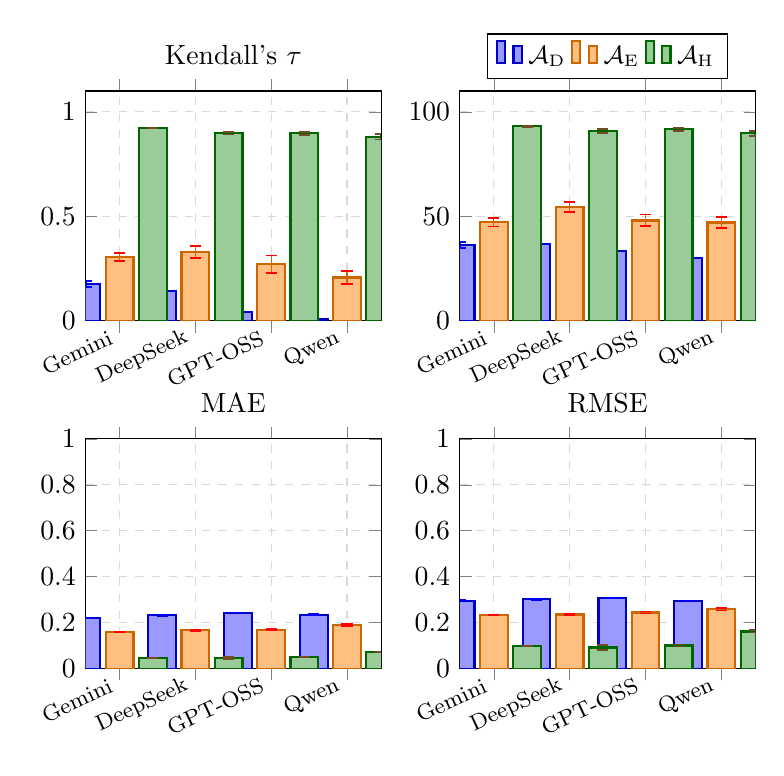
\begin{tikzpicture}
\begin{groupplot}[
    group style={
        group size=2 by 2,
        horizontal sep=1.0cm,
        vertical sep=1.5cm
    },
    width=0.44\columnwidth,
    height=4.5cm,
    ybar,
    enlarge x limits=0.15,
    symbolic x coords={Gemini, DeepSeek, GPT-OSS, Qwen},
    xtick=data,
    x tick label style={rotate=25, anchor=east, font=\footnotesize},
    grid=major,
    grid style={dashed, gray!30},
    error bars/y dir=both,
    error bars/y explicit,
    error bars/error mark options={
        rotate=90,
        line width=0.6pt,
        mark size=2pt
    }
]

\nextgroupplot[title={Kendall's $\tau$}, ymin=0, ymax=1.1]
\addplot+[fill=blue!40, draw=blue!80!black, thick] coordinates {
    (Gemini, 0.176) +- (0, 0.014) (DeepSeek, 0.144) +- (0, 0.041)
    (GPT-OSS, 0.041) +- (0, 0.045) (Qwen, 0.010) +- (0, 0.039)
};
\addplot+[fill=orange!50, draw=orange!80!black, thick] coordinates {
    (Gemini, 0.305) +- (0, 0.019) (DeepSeek, 0.328) +- (0, 0.029)
    (GPT-OSS, 0.270) +- (0, 0.042) (Qwen, 0.207) +- (0, 0.030)
};
\addplot+[fill=green!50!black!40, draw=green!40!black, thick] coordinates {
    (Gemini, 0.923) +- (0, 0.002) (DeepSeek, 0.897) +- (0, 0.005)
    (GPT-OSS, 0.897) +- (0, 0.007) (Qwen, 0.880) +- (0, 0.013)
};

\nextgroupplot[
    title={Top-1 (\%)}, ymin=0, ymax=110,
    legend style={font=\small, at={(0.5,1.05)}, anchor=south, legend columns=4}
]
\addplot+[fill=blue!40, draw=blue!80!black, thick] coordinates {
    (Gemini, 36.2) +- (0, 1.5) (DeepSeek, 36.7) +- (0, 3.1)
    (GPT-OSS, 33.3) +- (0, 2.4) (Qwen, 30.0) +- (0, 3.0)
};
\addplot+[fill=orange!50, draw=orange!80!black, thick] coordinates {
    (Gemini, 47.2) +- (0, 2.1) (DeepSeek, 54.5) +- (0, 2.3)
    (GPT-OSS, 48.0) +- (0, 2.8) (Qwen, 47.0) +- (0, 2.7)
};
\addplot+[fill=green!50!black!40, draw=green!40!black, thick] coordinates {
    (Gemini, 93.1) +- (0, 0.3) (DeepSeek, 90.8) +- (0, 0.9)
    (GPT-OSS, 91.6) +- (0, 0.8) (Qwen, 89.7) +- (0, 1.2)
};
\legend{$\mathcal{A}_{\text{D}}$, $\mathcal{A}_{\text{E}}$, $\mathcal{A}_{\text{H}}$}

\nextgroupplot[title={MAE}, ymin=0, ymax=1.0]
\addplot+[fill=blue!40, draw=blue!80!black, thick] coordinates {
    (Gemini, 0.220) +- (0, 0.002) (DeepSeek, 0.232) +- (0, 0.003)
    (GPT-OSS, 0.242) +- (0, 0.002) (Qwen, 0.235) +- (0, 0.002)
};
\addplot+[fill=orange!50, draw=orange!80!black, thick] coordinates {
    (Gemini, 0.159) +- (0, 0.001) (DeepSeek, 0.167) +- (0, 0.002)
    (GPT-OSS, 0.169) +- (0, 0.003) (Qwen, 0.191) +- (0, 0.004)
};
\addplot+[fill=green!50!black!40, draw=green!40!black, thick] coordinates {
    (Gemini, 0.048) +- (0, 0.001) (DeepSeek, 0.047) +- (0, 0.004)
    (GPT-OSS, 0.052) +- (0, 0.001) (Qwen, 0.072) +- (0, 0.002)
};

\nextgroupplot[title={RMSE}, ymin=0, ymax=1.0]
\addplot+[fill=blue!40, draw=blue!80!black, thick] coordinates {
    (Gemini, 0.296) +- (0, 0.002) (DeepSeek, 0.302) +- (0, 0.003)
    (GPT-OSS, 0.307) +- (0, 0.002) (Qwen, 0.295) +- (0, 0.002)
};
\addplot+[fill=orange!50, draw=orange!80!black, thick] coordinates {
    (Gemini, 0.233) +- (0, 0.001) (DeepSeek, 0.236) +- (0, 0.002)
    (GPT-OSS, 0.244) +- (0, 0.004) (Qwen, 0.259) +- (0, 0.006)
};
\addplot+[fill=green!50!black!40, draw=green!40!black, thick] coordinates {
    (Gemini, 0.100) +- (0, 0.001) (DeepSeek, 0.092) +- (0, 0.011)
    (GPT-OSS, 0.101) +- (0, 0.004) (Qwen, 0.162) +- (0, 0.005)
};

\end{groupplot}
\end{tikzpicture}
\caption{Overall performance by model (5-run mean $\pm$ std, 195 scenarios). Error bars show $\pm 1$ std across five runs.}
\label{fig:grouped_bars}
\end{figure}
\FloatBarrier

Figure~\ref{fig:grouped_bars} shows the architecture ordering is as expected. $\mathcal{A}_{\text{H}}$ dominates on every metric for all four models ($\tau \geq 0.88$, Top-1 $> 89\%$), $\mathcal{A}_{\text{E}}$ places second ($\tau \sim 0.2$--0.33), and $\mathcal{A}_{\text{D}}$ ranks third ($\tau$ near zero). Full per-model results by decision type appear in Appendix~\ref{app:per_model_results}; numerical values in Supplementary Material S2. Qwen ranks lowest across all three architectures, but the ordering of the other models is not consistent (Gemini leads DeepSeek under $\mathcal{A}_{\text{D}}$ but trails it under $\mathcal{A}_{\text{E}}$), and the gap between models is smaller for $\mathcal{A}_{\text{H}}$ (cost implications discussed in Section~\ref{sec:res-efficiency}).

Ranking metrics partly reflect a structural advantage of $\mathcal{A}_{\text{H}}$: the LLM estimates scenario-level parameters, while the calculator parses and scores the three alternatives deterministically. Because many extraction errors shift all alternatives together, they largely cancel in the ranking; MAE/RMSE and parameter-specific failure patterns therefore provide the stronger evidence of extraction fidelity. Additionally, the calculator having the correct formulas and methods from the beginning also increases base scores. 

Pairwise differences between architectures are significant under Wilcoxon signed-rank testing within each model taken separately. All 24 tests (two adjacent pairs, three metrics, four models) survive Holm correction; the three largest adjusted values are Gemini's $\mathcal{A}_{\text{D}}$-versus-$\mathcal{A}_{\text{E}}$ tests on $\tau$ and Top-1 ($p_{\mathrm{Holm}} = 0.0092$ each) and DeepSeek's on $\tau$ ($0.0018$), and every remaining test falls at or below $1.1 \times 10^{-4}$. No cross-model combination is reported: the four models score the same 195 scenarios against the same ground truth, so their per-scenario differences are positively dependent and a combination assuming independence would be anti-conservative. Gemini's median paired difference is exactly zero on both $\mathcal{A}_{\text{D}}$-versus-$\mathcal{A}_{\text{E}}$ ranking metrics, so its effect size is read from Cliff's $\delta$ ($-0.128$ on $\tau$, $-0.143$ on Top-1, both negligible) rather than from the median. GPT-OSS contributes $n = 194$ rather than 195 on the $\mathcal{A}_{\text{E}}$-versus-$\mathcal{A}_{\text{H}}$ comparison, one scenario dropping from the paired set. Full per-model results are in Supplementary Material S2.

ICC(2,1), Cliff's~$\delta$, and bootstrap comparisons (Supplementary Material S2) converge on the same conclusion: $\mathcal{A}_{\text{H}}$'s advantage holds consistently across models rather than depending on which model is used, though within-architecture residual variance remains substantial.

Score-level error and ranking outcome tell the same story from opposite ends. $\mathcal{A}_{\text{D}}$ individual scores routinely miss by more than 0.2 points and offer no actionable ranking information: it performs only marginally above random overall ($\tau = 0.093$, Top-1 $= 34.1\%$ against a $33.3\%$ chance baseline) and below random on Top-1 accuracy in 8 of the 12 model--decision-type combinations (6 of 12 by Kendall's $\tau$). $\mathcal{A}_{\text{E}}$'s score error falls between the other two architectures, usable for rough ranking but not reliable score comparison, and its ranking signal is correspondingly weak but non-random: better than chance but unreliable for any single decision. $\mathcal{A}_{\text{H}}$ predictions deviate by only 5--7\% on average (its RMSE/MAE ratio is the highest of the three architectures because a small number of shower scenarios requiring GPM estimation produce larger deviations), and this low score error translates into near-perfect ranking across all models, identifying the correct order in nearly every scenario and the best option nine times out of ten at the Top-1 level.

The mechanism behind $\mathcal{A}_{\text{D}}$'s failure is not the compression toward the middle of the scale predicted in Section~\ref{sec:lit-review}: $\mathcal{A}_{\text{D}}$ separates the three alternatives within a scenario more widely than the physics reference does, not less. Its mean within-scenario range of the MAVT aggregate is 0.181 for Qwen, 0.210 for GPT-OSS, 0.233 for Gemini, and 0.289 for DeepSeek, against 0.145 for the reference, a factor of 1.25 to 2.00 with a run-to-run standard deviation of 0.002--0.012; on HVAC energy cost the excess reaches 0.518 against the reference's 0.082. $\mathcal{A}_{\text{D}}$ orders the alternatives confidently and wrongly rather than failing to discriminate between them.

\FloatBarrier
\subsection{Baseline Comparison}
\label{sec:res-baselines}
Table~\ref{tab:incremental-contribution} extends the comparison beyond the three LLM architectures to two non-LLM baselines, all evaluated on the same 195-scenario test set. Metrics are reported as per-type arithmetic means (averaging HVAC, Appliance, and Shower results equally) so that each decision type contributes equally regardless of scenario count; this prevents FixedDefault's strong HVAC performance from inflating its aggregate score. The two non-LLM rows of Table~\ref{tab:incremental-contribution} are pooled over all 195 scenarios instead, because that is the form in which both baselines are reported elsewhere in the paper; for FixedDefault the two aggregations differ by 0.0028 on Top-1 (0.7026 pooled against 0.6998 per-type) and 0.0035 on $\tau$ (0.6137 against 0.6102), so the choice moves no comparison in the table. The Fixed-Default baseline ranks the same three alternatives as every other system, but substitutes one fixed value for each withheld engineering parameter before calling the same physics calculators used by the ground truth: R-value 15, SEER 13, and HVAC age 13 years for HVAC; a per-appliance-type kWh/cycle (0.55 washer, 2.10 dryer, 1.00 dishwasher) and a 7\,p.m.\ baseline run time for Appliance; and 2.5\,GPM, a 50-gallon tank, and a 120\textdegree{}F heater setpoint for Shower. It performs no per-scenario inference, so it isolates what calculator access buys with no estimation at all.

\begin{table*}[htbp]
\begin{threeparttable}
  \footnotesize
  \centering
  \textbf{Incremental contribution over Fixed-Default baseline}
  \begin{tabular}{lcccc}
    \toprule
    System & Top-1 & $\Delta$ vs FixedDef & Kendall $\tau$ & $\Delta$ vs FixedDef \\
    \midrule
    FixedDefault & 0.7026 & $0.0000$ & 0.6137 & $0.0000$ \\
    NearestNeighbor & 0.5692 & $-0.1334$ & 0.3709 & $-0.2428$ \\
    \addlinespace
    $\mathcal{A}_{\text{D}}$ (best: Gemini) & 0.371 & $-0.332$ & 0.193 & $-0.421$ \\
    $\mathcal{A}_{\text{D}}$ (worst: Qwen)   & 0.301 & $-0.402$ & 0.012 & $-0.602$ \\
    \addlinespace
    $\mathcal{A}_{\text{E}}$ (best: DeepSeek) & 0.552 & $-0.150$ & 0.341 & $-0.272$ \\
    $\mathcal{A}_{\text{E}}$ (worst: Qwen)    & 0.472 & $-0.231$ & 0.209 & $-0.405$ \\
    \addlinespace
    $\mathcal{A}_{\text{H}}$ (best: Gemini) & 0.928 & $+0.226$ & 0.920 & $+0.306$ \\
    $\mathcal{A}_{\text{H}}$ (worst: Qwen)  & 0.898 & $+0.195$ & 0.879 & $+0.266$ \\
    \bottomrule
  \end{tabular}
\end{threeparttable}
\caption{Top-1 accuracy and Kendall's~$\tau$ for each system. The LLM rows are per-type arithmetic means; the two non-LLM baseline rows are pooled over all 195 scenarios, which moves them by less than 0.004 relative to their per-type means. Best and worst model shown for LLM architectures.}
\label{tab:incremental-contribution}
\end{table*}
\FloatBarrier

FixedDefault achieves high HVAC accuracy (the R-15/SEER-13 defaults are close to the corpus centre for most Pennsylvania scenarios) and strong Shower ranking ($\tau = 0.800$, because the 2.5-GPM, 50-gallon, 120\textdegree{}F defaults are near-optimal for most scenarios), but collapses on Appliance ($\tau = 0.097$), yielding a per-type average of $\tau = 0.610$ and the pooled $\tau = 0.614$ that Table~\ref{tab:incremental-contribution} reports. NearestNeighbor ($k=3$ majority vote over the RAG corpus) achieves a pooled $\tau = 0.371$ (Table~\ref{tab:incremental-contribution}); unmodified exemplar copying provides partial but limited ranking signal.

This baseline is important because it shows that the benchmark is not merely rewarding calculator use. A fixed physics-based heuristic can perform well where its default happens to match the domain, but it does not adapt reliably across decision types. The LLM architectures must demonstrate flexible reasoning, not just calculator access, to outperform a fixed default.

A second check bounds how much of the ranking task the ground truth's own structure gives away. If one criterion alone recovered the reference winner, an architecture could rank correctly without weighing four criteria at all. No criterion does so across decision types. Over the 195 Test scenarios, comfort taken alone is the argmax for the reference winner in 85.7\% of HVAC and 92.3\% of Appliance scenarios but only 18.3\% of Shower scenarios, below the 33.3\% chance level for three alternatives; energy cost inverts that pattern at 10.0\% for HVAC and 75.0\% for Shower. Environmental impact tracks energy cost (10.0\%, 46.2\%, 75.0\% for HVAC, Appliance, Shower) and practicality is informative on Appliance alone (27.1\%, 90.8\%, 20.0\%). The same statistic computed on the full 285-scenario corpus preserves every ordering and moves no cell by more than 6.5 points, so the bound does not depend on the Test/RAG split.

\FloatBarrier
\subsection{Criterion-Level Error}
\label{sec:res-error}
\begin{figure*}[htbp]
	\centering
	\plotCriterionMAEByModel
	\caption{MAE by criterion and model (5-run mean, 195 scenarios each). Each line is one model; the x-axis is architecture ($\mathcal{A}_{\text{D}}$~$\rightarrow$~$\mathcal{A}_{\text{E}}$~$\rightarrow$~$\mathcal{A}_{\text{H}}$).}
\label{fig:mae_criterion}
\end{figure*}

Figure~\ref{fig:mae_criterion} breaks MAE down by criterion and model (full numerical values in Supplementary Material S2). $\mathcal{A}_{\text{H}}$ achieves near-zero error on Comfort and Practicality across all four models. Again, this is expected: the calculator handles both criteria deterministically, with the LLM only estimating scenario-level parameters (occupancy, tank size) that shift all three alternatives together.

Error concentrates on Energy Cost and Environmental Impact for all three architectures. Even $\mathcal{A}_{\text{H}}$'s weakest model outperforms the best models of $\mathcal{A}_{\text{D}}$ and $\mathcal{A}_{\text{E}}$ on these criteria. The Environmental--Energy Cost gap persists across architectures. Shower environmental impact is measured in gallons of water while HVAC and Appliance environmental impact are measured in lbs\,CO\textsubscript{2}, so the pooled environmental MAE should not be read as error in a single physical unit.

Table~\ref{tab:score_duplication} reports the share of scored alternatives in which each architecture returned the identical value for the energy-cost and environmental criteria. The rates track the reference's correlation structure for Gemini and DeepSeek and do not for Qwen: Gemini duplicates 76.6\% ($\mathcal{A}_{\text{D}}$) and 99.0\% ($\mathcal{A}_{\text{E}}$) of HVAC scores, 96.6\% ($\mathcal{A}_{\text{D}}$) and 68.1\% ($\mathcal{A}_{\text{E}}$) of Shower scores, and 15.1\% ($\mathcal{A}_{\text{D}}$) and 21.4\% ($\mathcal{A}_{\text{E}}$) of Appliance scores; DeepSeek's $\mathcal{A}_{\text{E}}$ rates follow the same ordering (95.7\%, 67.4\%, 28.2\%), while Qwen duplicates 98.9--99.0\% of HVAC scores and 92.0--100.0\% of Shower scores ($\mathcal{A}_{\text{D}}$/$\mathcal{A}_{\text{E}}$) and 95.6\% ($\mathcal{A}_{\text{D}}$) and 61.9\% ($\mathcal{A}_{\text{E}}$) of Appliance scores. On HVAC and Shower the reference's cost and environmental quantities are collinear within each scenario because the parameters that separate them (the occupancy-resolved emissions factor for HVAC, flow rate and heater setpoint for Shower) are scenario-level and identical across the three alternatives, so a duplicated pair follows the reference structure there; the within-scenario correlations are reported in Section~\ref{sec:mavt-design}. This is one measurement on a four-model sample, and on HVAC and Shower the criterion-level cost and environmental errors in Figure~\ref{fig:mae_criterion} are not independent measurements.

\begin{table*}[htbp]
\begin{threeparttable}
  \footnotesize
  \centering
  \textbf{Cost--environmental score duplication rate}
  \begin{tabular}{llccc}
    \toprule
    Model & Architecture & HVAC (\%) & Shower (\%) & Appliance (\%) \\
    \midrule
    Gemini 3.5 Flash & $\mathcal{A}_{\text{D}}$ & 76.6 $\pm$ 2.1 & 96.6 $\pm$ 1.3 & 15.1 $\pm$ 2.0 \\
    \addlinespace
    Gemini 3.5 Flash & $\mathcal{A}_{\text{E}}$ & 99.0 $\pm$ 0.7 & 68.1 $\pm$ 1.5 & 21.4 $\pm$ 0.8 \\
    GPT-OSS 20B & $\mathcal{A}_{\text{D}}$ & 61.8 $\pm$ 3.6 & 99.2 $\pm$ 0.5 & 93.7 $\pm$ 1.9 \\
    \addlinespace
    GPT-OSS 20B & $\mathcal{A}_{\text{E}}$ & 91.4 $\pm$ 2.2 & 63.1 $\pm$ 2.1 & 41.2 $\pm$ 2.8 \\
    Qwen3.5 9B & $\mathcal{A}_{\text{D}}$ & 99.0 $\pm$ 0.8 & 100.0 $\pm$ 0.0 & 95.6 $\pm$ 1.5 \\
    \addlinespace
    Qwen3.5 9B & $\mathcal{A}_{\text{E}}$ & 98.9 $\pm$ 0.8 & 92.0 $\pm$ 0.5 & 61.9 $\pm$ 2.4 \\
    DeepSeek V4 Flash & $\mathcal{A}_{\text{D}}$ & 55.5 $\pm$ 5.2 & 77.3 $\pm$ 4.2 & 58.7 $\pm$ 2.3 \\
    \addlinespace
    DeepSeek V4 Flash & $\mathcal{A}_{\text{E}}$ & 95.7 $\pm$ 1.2 & 67.4 $\pm$ 2.3 & 28.2 $\pm$ 1.4 \\
    \bottomrule
  \end{tabular}
  \begin{tablenotes}
    \item Five-run mean $\pm$ standard deviation of the percentage of scored
    alternatives in which the architecture returned the identical value for
    energy cost and environmental impact (equal within floating-point tolerance).
    Alternatives carrying a failed score are excluded before computing the rate.
  \end{tablenotes}
\end{threeparttable}
\caption{Share of scored alternatives in which the architecture assigned
identical energy-cost and environmental scores, by decision type.}
\label{tab:score_duplication}
\end{table*}

\FloatBarrier
\subsection{Extraction Accuracy and Error Propagation}
\label{sec:res-extraction}
Score-level error measures how well $\mathcal{A}_{\text{H}}$ reproduces the reference calculator's output, but it does not separate two distinct questions: how accurately the LLM estimates each withheld engineering parameter, and whether an estimation error changes the recommendation. Table~\ref{tab:extraction_accuracy} reports both. Extracted parameters were compared against the scenario source values for all 195 test scenarios, and a counterfactual analysis re-ran the calculator with each erroneous parameter substituted individually, holding all others at their true values, to measure how often the top-ranked alternative changes.

Absolute extraction error is substantial. HVAC equipment age is estimated to within 6.1--8.5 years on average and shower tank size to within 6.7--8.9 gallons, both large fractions of the plausible range. Categorical extraction is more reliable: appliance type and baseline run time are recovered essentially perfectly, while HVAC occupancy context reaches only 75--81\%.

That error rarely propagates to the decision. For most parameters the conditional probability that an extraction error flips the top-ranked alternative sits below 0.09, and for HVAC equipment age it is zero across all four models. The reason is structural: the LLM estimates scenario-level parameters that enter all three alternatives identically, so an error shifts the whole choice set and largely cancels in the ranking. Shower GPM is the consistent exception, carrying the highest flip probability for every model (0.133--0.233), roughly two to three times the next-largest parameter for three of the four models and about 1.5 times for Qwen. GPM is the one extracted parameter that must map a discrete homeowner-facing tier (low\_flow, standard, high\_flow) onto a continuous value that scales both energy and water volume directly, and it is the parameter behind the Shower results being $\mathcal{A}_{\text{H}}$'s weakest decision type (Section~\ref{sec:res-bytype}). This localizes the error-cancellation mechanism rather than assuming it: ranking robustness is real, but it rests on common-mode error, and it weakens precisely where a parameter is both decision-critical and recovered from a coarse proxy.

\begin{table*}[htbp]
\begin{threeparttable}
\footnotesize
\centering
\textbf{Extraction accuracy and counterfactual top-1 sensitivity}
\renewcommand{\arraystretch}{1.15}
\setlength{\tabcolsep}{4pt}
\begin{tabular}{llcccccccc}
\toprule
 & & \multicolumn{4}{c}{MAE} & \multicolumn{4}{c}{$P(\text{top-1 change} \mid \text{error})$} \\
\cmidrule(lr){3-6}\cmidrule(lr){7-10}
Type & Parameter & GPT-OSS & Qwen & DeepSeek & Gemini & GPT-OSS & Qwen & DeepSeek & Gemini \\
\midrule
HVAC & R-value & 3.594 & 3.699 & 2.312 & 1.766 & 0.015 & 0.086 & 0.015 & 0.000 \\
HVAC & SEER & 2.135 & 1.585 & 1.602 & 1.313 & 0.049 & 0.033 & 0.032 & 0.075 \\
HVAC & HVAC age (yr) & 8.455 & 6.105 & 8.462 & 7.640 & 0.000 & 0.000 & 0.000 & 0.000 \\
Appliance & kWh/cycle & 0.425 & 0.975 & 0.341 & 0.541 & 0.016 & 0.066 & 0.016 & 0.031 \\
Shower & GPM & 0.256 & 0.271 & 0.368 & 0.367 & \textbf{0.152} & \textbf{0.133} & \textbf{0.185} & \textbf{0.233} \\
Shower & Tank size (gal) & 8.100 & 8.933 & 6.933 & 6.733 & 0.000 & 0.026 & 0.025 & 0.000 \\
Shower & Heater setpoint (\textdegree{}F) & 4.717 & 4.583 & 8.317 & 4.583 & 0.042 & 0.050 & 0.062 & 0.050 \\
\bottomrule
\end{tabular}
\setlength{\tabcolsep}{6pt}
\renewcommand{\arraystretch}{1.0}
\begin{tablenotes}
\item Numeric parameters only; all 195 test scenarios matched for every model. Categorical accuracy: appliance type 100\% (GPT-OSS, Qwen, DeepSeek) and 93.8\% (Gemini); baseline time 100\% for all models; HVAC occupancy context 75.4\%, 78.6\%, 81.4\%, and 80.0\% respectively. Counterfactual probabilities are conditional on the parameter being mis-estimated, with each parameter varied individually.
\end{tablenotes}
\end{threeparttable}
\caption{Per-parameter extraction error and the probability that an extraction error changes the top-ranked alternative.}
\label{tab:extraction_accuracy}
\end{table*}

\FloatBarrier
\subsection{Isolating the Contribution of Extraction}
\label{sec:res-paramprov}
The error-cancellation mechanism in Section~\ref{sec:res-extraction} raises a sharper objection: if extraction errors largely cancel in the ranking, perhaps $\mathcal{A}_{\text{H}}$ ranks well simply because it has access to the reference calculator, and the LLM's parameter estimates contribute little. A parameter-provenance ablation separates the two (design and significance-testing methodology in Section~\ref{sec:hybrid-ablation-methods}). Three arms are scored by the same calculators over the same 195 test scenarios, differing only in where the withheld engineering parameters come from: the scenario's true values, the values the LLM actually returned, and a single corpus-median constant per parameter reused for every scenario. The first arm is the reference ranking itself and so is the ceiling; the third performs no per-scenario inference at all and so isolates what calculator access alone buys. Table~\ref{tab:param_provenance} reports the result.

Calculator access alone is not sufficient. With no per-scenario inference, the median-parameter arm reaches $\tau = 0.641$ and Top-1 of 76.9\%, well above chance but far below the published $\mathcal{A}_{\text{H}}$ results. LLM extraction lifts this to $\tau = 0.897$--$0.921$ and Top-1 of 91.3--94.3\%, a gain of 0.26--0.28 in $\tau$ attributable to extraction rather than to the calculator. The extracted arm's $\tau$ falls within 0.03 of the main-text $\mathcal{A}_{\text{H}}$ values in Figure~\ref{fig:grouped_bars} for every model, which validates the ablation harness against known results. The remaining gap to the ceiling, about 0.08--0.10 in $\tau$, is the headroom a better estimator could recover. Extraction is therefore doing substantive work: the common-mode cancellation identified above acts on informative estimates, not on noise.

\begin{table*}[htbp]
\begin{threeparttable}
\footnotesize
\centering
\textbf{Parameter-provenance ablation}
\renewcommand{\arraystretch}{1.15}
\begin{tabular}{llccc}
\toprule
Model & Parameter source & $\tau$ & Top-1 & MAE \\
\midrule
GPT-OSS & True (ceiling) & 1.000 & 1.000 & 0.000 \\
GPT-OSS & LLM-extracted & 0.921 & 0.943 & 0.046 \\
GPT-OSS & Corpus median & 0.641 & 0.769 & 0.122 \\
\midrule
Qwen & True (ceiling) & 1.000 & 1.000 & 0.000 \\
Qwen & LLM-extracted & 0.897 & 0.913 & 0.066 \\
Qwen & Corpus median & 0.641 & 0.769 & 0.122 \\
\midrule
DeepSeek & True (ceiling) & 1.000 & 1.000 & 0.000 \\
DeepSeek & LLM-extracted & 0.904 & 0.913 & 0.041 \\
DeepSeek & Corpus median & 0.641 & 0.769 & 0.122 \\
\midrule
Gemini & True (ceiling) & 1.000 & 1.000 & 0.000 \\
Gemini & LLM-extracted & 0.921 & 0.928 & 0.047 \\
Gemini & Corpus median & 0.641 & 0.769 & 0.122 \\
\bottomrule
\end{tabular}
\renewcommand{\arraystretch}{1.0}
\begin{tablenotes}
\item All arms scored by the same reference calculators over the same 195 test scenarios; the arms differ only in the source of the withheld engineering parameters. The true-parameter arm reproduces the reference ranking exactly by construction, which serves as a correctness check on the harness. The corpus-median arm uses one constant per parameter and no model output, so it is identical across models, and the four identical 0.641 / 0.769 / 0.122 rows serve as a second correctness check on the harness. Scenarios whose extraction failed are excluded from that arm rather than defaulted; the extracted arm scored 194 of 195 scenarios for GPT-OSS and 195 for the other three models.
\end{tablenotes}
\end{threeparttable}
\caption{Ranking accuracy of $\mathcal{A}_{\text{H}}$ with true, LLM-extracted, and corpus-median hidden parameters.}
\label{tab:param_provenance}
\end{table*}

Friedman tests confirm the three arms differ by more than run-to-run noise for every model on every metric ($\chi^2_2$ ranging from 52.5 to 305.3, all $p_{\text{Holm}} < 10^{-11}$ across the twelve-test family described in Section~\ref{sec:hybrid-ablation-methods}). Post-hoc Wilcoxon signed-rank tests isolate where that difference sits. Extracted beats default\_params on Kendall's $\tau$ for all four models ($p_{\text{Holm}} < 10^{-6}$, Cliff's $\delta$ between $-0.22$ and $-0.24$, small) and on MAE ($p_{\text{Holm}} < 10^{-10}$, $\delta$ between 0.35 and 0.48, medium to large); the Top-1 comparison is significant for all four models but the effect size is small for GPT-OSS ($\delta=-0.175$) and Gemini ($\delta=-0.159$) and negligible for DeepSeek and Qwen ($\delta=-0.144$), since Top-1 is coarser than $\tau$ and both arms already place the correct alternative first most of the time.

The remaining gap to the ceiling tells a different story. Extracted differs from true\_params significantly on all three metrics for all four models, but on Kendall's $\tau$ and Top-1 the effect size is negligible for every model ($|\delta| \leq 0.118$); only on MAE is the gap large ($\delta > 0.88$ for all four models). With $n=195$ paired scenarios, a small and consistent shortfall is enough to reach significance without being practically large. Extraction has closed nearly all of the ranking gap to the ceiling; what remains is a score-calibration gap, consistent with the RMSE/MAE discussion in Section~\ref{sec:res-error}.

This comparison is hard to dismiss as an artifact. Every arm is scored by the same calculator code used for the ground truth and by $\mathcal{A}_{\text{H}}$ itself, so the arms differ only in one input, not in scoring logic; the ablation draws on data already collected for the main benchmark rather than a new run assembled for this comparison, and reproduces the published $\mathcal{A}_{\text{H}}$ numbers almost exactly when scored with extracted parameters; and the significance pipeline reuses the same reviewed Friedman/Holm/Cliff's-$\delta$ code as the RAG and prompt ablations (Sections~\ref{sec:rag-ablation-methods}, \ref{sec:prompt-ablation-methods}).

This ablation answers the objection raised in Section~\ref{sec:res-extraction}: as shown above, $\mathcal{A}_{\text{H}}$'s advantage over $\mathcal{A}_{\text{D}}$ and $\mathcal{A}_{\text{E}}$ is not simply that it has a calculator, since extraction accounts for the 0.26--0.28 gap in $\tau$ between the median-parameter arm and full performance. Parameter extraction and deterministic scoring are both doing real work, and neither one alone would suffice.

\FloatBarrier
\subsection{Performance by Decision Type}
\label{sec:res-bytype}
Table~\ref{tab:item7} reports $\tau$ by decision type; per-decision-type breakdowns for both Kendall's $\tau$ and Top-1 accuracy appear in Appendix~\ref{app:decision_type_full_figures}. $\mathcal{A}_{\text{H}}$ excels across all three decision types for every model. Shower is the weakest due to GPM estimation limits, still far above the other architectures.

\begin{table*}[t]
\begin{threeparttable}
\footnotesize
\centering
\textbf{Ranking accuracy by decision type}
\renewcommand{\arraystretch}{1.15}
\setlength{\tabcolsep}{4pt}
\begin{tabular}{lcccccc}
\toprule
 & \multicolumn{2}{c}{$\mathcal{A}_{\text{D}}$} & \multicolumn{2}{c}{$\mathcal{A}_{\text{E}}$} & \multicolumn{2}{c}{$\mathcal{A}_{\text{H}}$} \\
\cmidrule(lr){2-3}\cmidrule(lr){4-5}\cmidrule(lr){6-7}
Decision Type & $\tau$ & Top-1 (\%) & $\tau$ & Top-1 (\%) & $\tau$ & Top-1 (\%) \\
\midrule
HVAC & & & & & & \\
\quad Best & 0.135 (O) & 39.7 (O) & 0.265 (O) & 46.9 (O) & \textbf{0.977 (G)} & \textbf{96.6 (G)} \\
\quad Worst & $-0.102$ (D) & 19.8 (D) & $-0.116$ (G) & 15.3 (G) & \textbf{0.881 (Q)} & \textbf{87.4 (Q)} \\
Appliance & & & & & & \\
\quad Best & 0.029 (D) & 31.7 (D) & 0.417 (D) & 70.2 (D) & \textbf{0.975 (D)} & \textbf{98.5 (D)} \\
\quad Worst & $-0.147$ (O) & 26.8 (O) & $-0.048$ (O) & 30.5 (O) & \textbf{0.906 (Q)} & \textbf{92.9 (Q)} \\
Shower & & & & & & \\
\quad Best & 0.633 (G) & 61.0 (G) & 0.766 (G) & 75.5 (G) & \textbf{0.851 (Q)} & \textbf{89.0 (Q)} \\
\quad Worst & 0.069 (Q) & 34.3 (Q) & 0.236 (Q) & 48.3 (Q) & \textbf{0.784 (O)} & \textbf{82.0 (O)} \\
\bottomrule
\end{tabular}
\setlength{\tabcolsep}{6pt}
\renewcommand{\arraystretch}{1.0}
\end{threeparttable}
\caption{5-run per-run-then-average, showing best and worst model per cell (G = Gemini, D = DeepSeek, O = GPT-OSS, Q = Qwen). Per-model results by decision type appear in Appendix~\ref{app:per_model_results}.}
\label{tab:item7}
\end{table*}

$\mathcal{A}_{\text{E}}$ shows wide model-level variance on HVAC, performs strongest on Shower across all models, and depends primarily on duration and flow rate---fewer interacting variables than HVAC load calculations or appliance TOU scheduling---so the exemplar's calibration anchor is more effective here.

The margin between architectures varies with task dimensionality. HVAC---the highest-dimensional task (insulation, SEER, age, occupancy, square footage, outdoor temperature)---shows the widest gap between $\mathcal{A}_{\text{H}}$ and $\mathcal{A}_{\text{E}}$ because correct ranking requires accurate joint estimation of multiple parameters. Shower---the lowest-dimensional (duration, flow rate, tank size)---shows the narrowest gap because a single well-estimated parameter can carry the ranking. Appliance results for $\mathcal{A}_{\text{H}}$ track extraction quality since the baseline time parameter varies across alternatives, making it the strongest test of extraction fidelity.

$\mathcal{A}_{\text{D}}$ is near-random or below on HVAC and Appliance for all models. Shower diverges: the two strongest models show meaningful positive correlation while the two weakest remain near-random. The Appliance $\mathcal{A}_{\text{D}}$--$\mathcal{A}_{\text{E}}$ comparison carries an anchor asymmetry: $\mathcal{A}_{\text{D}}$'s Appliance anchors hand the model the time-of-use rate periods and the overnight emissions minimum, which $\mathcal{A}_{\text{E}}$'s prompt omits.

\FloatBarrier
\subsection{Sensitivity Analysis}
\label{sec:res-sensitivity}

To test the stability of the ranking results, both the ground-truth ranking and the architecture rankings were recomputed under a range of alternative weight vectors: an equal-weight vector ($w_j = 0.25$ for all $j$), and the entropy- and MEREC-derived vectors of Appendix~\ref{app:weights}, applied pooled and per decision type. Single-criterion $\pm 0.05$ perturbations of the design vector are not reported: they move the $\mathcal{A}_{\text{E}} - \mathcal{A}_{\text{D}}$ gap only within $0.104$--$0.258$ across the four models and never reverse its sign, whereas the MEREC HVAC vector drives it to $-0.072$ for Gemini, so they probe a strictly narrower range than the data-derived vectors already shown and cannot establish weight robustness on their own.

\begin{table*}[htbp]
\begin{threeparttable}
\footnotesize
\centering
\textbf{Sensitivity analysis: Kendall's $\tau$ by model under reweighting}
\renewcommand{\arraystretch}{1.15}
\setlength{\tabcolsep}{4pt}
\begin{tabular}{@{} l rrr rrr rrr rrr @{}}
\toprule
 & \multicolumn{3}{c}{Gemini} & \multicolumn{3}{c}{DeepSeek} & \multicolumn{3}{c}{GPT-OSS} & \multicolumn{3}{c}{Qwen} \\
\cmidrule(lr){2-4}\cmidrule(lr){5-7}\cmidrule(lr){8-10}\cmidrule(lr){11-13}
\textbf{Weight vector} & $\mathcal{A}_{\text{D}}$ & $\mathcal{A}_{\text{E}}$ & $\mathcal{A}_{\text{H}}$ & $\mathcal{A}_{\text{D}}$ & $\mathcal{A}_{\text{E}}$ & $\mathcal{A}_{\text{H}}$ & $\mathcal{A}_{\text{D}}$ & $\mathcal{A}_{\text{E}}$ & $\mathcal{A}_{\text{H}}$ & $\mathcal{A}_{\text{D}}$ & $\mathcal{A}_{\text{E}}$ & $\mathcal{A}_{\text{H}}$ \\
\midrule
Design (baseline)  & 0.176 & 0.305 & 0.923 & 0.144 & 0.328 & 0.897 & 0.041 & 0.270 & 0.897 & 0.010 & 0.207 & 0.880 \\
Equal              & 0.309 & 0.389 & 0.925 & 0.113 & 0.316 & 0.914 & 0.079 & 0.281 & 0.891 & $-$0.027 & 0.238 & 0.890 \\
\midrule
Entropy pooled     & 0.197 & 0.331 & 0.908 & 0.123 & 0.324 & 0.865 & 0.039 & 0.268 & 0.870 & 0.006 & 0.198 & 0.842 \\
Entropy per-type   & 0.167 & 0.333 & 0.913 & 0.089 & 0.355 & 0.893 & 0.041 & 0.272 & 0.885 & $-$0.005 & 0.215 & 0.888 \\
\midrule
MEREC pooled       & \textbf{0.655} & 0.616 & 0.932 & 0.219 & 0.428 & 0.945 & 0.234 & 0.331 & 0.929 & 0.000 & 0.259 & 0.941 \\
MEREC per-type     & 0.602 & 0.634 & 0.939 & 0.308 & 0.389 & 0.931 & 0.162 & 0.387 & 0.908 & 0.042 & 0.271 & 0.925 \\
MEREC HVAC vector  & \textbf{0.676} & 0.604 & 0.971 & 0.333 & 0.440 & 0.971 & 0.275 & 0.441 & 0.960 & 0.064 & 0.279 & 0.967 \\
\bottomrule
\end{tabular}
\renewcommand{\arraystretch}{1.0}
\setlength{\tabcolsep}{6pt}
\begin{tablenotes}
\footnotesize
\item Both the reference ranking and the architecture ranking are recomputed under each vector, because a MAVT reference is defined by its weights. Bold marks the two cells in which $\mathcal{A}_{\text{D}}$ exceeds $\mathcal{A}_{\text{E}}$; both occur for Gemini under MEREC vectors. Top-1 accuracy for the same cells appears in Supplementary Material S2.
\end{tablenotes}
\end{threeparttable}
\caption{Kendall's $\tau$ by model and architecture under seven weight vectors. No value is pooled across models.}
\label{tab:sensitivity_by_model}
\end{table*}

$\mathcal{A}_{\text{H}}$'s advantage over $\mathcal{A}_{\text{E}}$ is unconditional: it holds in all 28 model $\times$ weight-vector cells, by a margin of at least $0.305$ Kendall's $\tau$. The $\mathcal{A}_{\text{E}}$ advantage over $\mathcal{A}_{\text{D}}$ is not. It survives the design, equal and entropy vectors in all four models, but MEREC weights narrow it sharply and in two cells reverse it: $\mathcal{A}_{\text{D}}$ overtakes $\mathcal{A}_{\text{E}}$ for Gemini under both the MEREC HVAC vector ($0.676$ vs.\ $0.604$) and MEREC pooled ($0.655$ vs.\ $0.616$). Every such case is a MEREC vector, which loads onto Comfort (0.663 for HVAC against the design's 0.200), the one criterion $\mathcal{A}_{\text{D}}$ estimates about as well as $\mathcal{A}_{\text{E}}$ does. The $\mathcal{A}_{\text{E}} > \mathcal{A}_{\text{D}}$ result should therefore be read as conditional on weighting that gives substantial mass to cost and emissions, which the design vector and the entropy vectors both do and MEREC does not. Per-model results appear in Supplementary Material S2.

A second check varies the value-function curvature rather than the weights. Recomputing the ground-truth scores with the logarithmic shape parameter $\alpha$ swept over $\{1.0,\,1.2,\,1.5,\,2.0\}$ (1.0 is the linear function) holds the weight vector at baseline and leaves the architecture scores untouched. For Gemini the ordering $\mathcal{A}_{\text{H}} > \mathcal{A}_{\text{E}} > \mathcal{A}_{\text{D}}$ is invariant across all four values, with Kendall's $\tau$ for $\mathcal{A}_{\text{D}}/\mathcal{A}_{\text{E}}/\mathcal{A}_{\text{H}}$ equal to 0.1788/0.2935/0.9097 at $\alpha = 1.0$, 0.1795/0.3082/0.9268 at $\alpha = 1.2$, 0.1761/0.3047/0.9234 at $\alpha = 1.5$, and 0.1767/0.3012/0.9131 at $\alpha = 2.0$.

The sensitivity analysis reweights both sides of the comparison: each arm recomputes the ground-truth weighted scores and the architecture weighted scores from the same vector. $\mathcal{A}_{\text{H}}$'s per-criterion scores originate from the reference calculator modules, so the two reweighted vectors are near-identical and $\mathcal{A}_{\text{H}}$'s invariance across vectors reflects architecture structure rather than evidence about the weight vector. The informative comparison is $\mathcal{A}_{\text{E}}$ against $\mathcal{A}_{\text{D}}$, whose criterion scores both differ substantively from the reference; Table~\ref{tab:sensitivity_by_model} shows that comparison is weight-robust across the design, equal and entropy vectors and not under MEREC.

\FloatBarrier
\subsection{RAG Ablation}
\label{sec:rag-ablation}
\begin{figure*}[htbp]
	\centering
	\plotRagAblation
	\caption{RAG ablation results: Kendall's $\tau$ by configuration and model on the full 90-scenario RAG corpus. Configurations are ordered by overall $\tau$. Dashed line marks $\tau = 0$.}
\label{fig:rag_ablation}
\end{figure*}

The RAG ablation (design in Section~\ref{sec:rag-ablation-methods}, full values in Supplementary Material S2) produced the following findings. Unlike the corpus-level \texttt{NearestNeighbor} baseline in Section~\ref{sec:res-baselines} ($k=3$ majority vote, evaluated on the 195-scenario test set), this offline baseline performs leave-one-out retrieval within the 90-scenario RAG corpus itself and assigns the retrieved scenario's score directly without LLM rescoring or voting, yielding $\tau = 0.001$ (95\% CI: $[-0.173,\, 0.175]$), indistinguishable from zero and confirming that naive exemplar copying provides no ranking signal.

Exemplar content matters in every model; retrieval depth matters in one. Removing scores drops $\tau$ to 0.073 for DeepSeek (from a control of 0.489), 0.204 for Gemini (from 0.387), 0.061 for GPT-OSS (from 0.187), and 0.071 for Qwen (from 0.154), while removing hidden engineering parameters moves $\tau$ far less and in both directions (0.391, 0.437, 0.175, and 0.273 for the same four models). Only DeepSeek and Gemini carry a Kendall's $\tau$ omnibus that survives the 16-test Friedman family, and within those two the top cluster separates for DeepSeek alone: its $k=1$ arm scores below the $k=3$ control at $p_{\text{Holm}} = 0.003$ (Cliff's $\delta = 0.247$, small), whereas Gemini's six top-cluster pairs all sit at $p_{\text{Holm}} \geq 0.35$. Removing exemplar scores or drawing random exemplars degrades score accuracy in every model: top-cluster MAE stays within 0.069--0.118 across the four models, while descriptions without scores (0.131--0.158) and random exemplars (0.127--0.163) approach half again the error. $k=1$ remains the recommended production setting on cost grounds for three of the four models, whose $k{=}1$ minus $k{=}3$ Kendall's $\tau$ CI contains zero: Gemini $[-0.163,\,0.142]$, GPT-OSS $[-0.128,\,0.228]$, and Qwen $[-0.047,\,0.326]$. DeepSeek is the exception, whose difference of $-0.32$ carries a CI ($[-0.471,\,-0.161]$) that excludes zero; an interval computed over the four models pooled contains zero ($[-0.120,\,0.052]$), so the pooled interval conceals this per-model reversal. $k=1$ is therefore recommended subject to a per-model check that retrieval depth does not degrade that model's ranking.

\FloatBarrier
\subsection{Prompt Sensitivity}
\label{sec:prompt-ablation}

A reviewer may reasonably ask whether the reported architecture ordering reflects the design of $\mathcal{A}_{\text{D}}$ and $\mathcal{A}_{\text{E}}$ or the particular prompts used to implement them. To separate the two, we re-ran both architectures under three controlled prompt perturbations across four models: removing the anchors from the scoring instructions (no\_anchors), adding an explicit chain-of-thought scaffold before the JSON response (cot\_scaffold), and rescaling the response range from 0--1 to 0--10 (scale\_0\_10). The full matrix comprises 28 architecture--model--variant cells, 156 runs, and 30{,}420 scenario-level observations. $\mathcal{A}_{\text{E}}$ ships without anchors, so no\_anchors has no $\mathcal{A}_{\text{E}}$ arm and those strata compare three variants rather than four. The harness re-declares the shipped prompts rather than importing them and asserts at startup that its control arm matches the deployed text, so a drift between the ablation and the production prompt fails loudly instead of silently weakening the baseline.

\begin{table*}[htbp]
\begin{threeparttable}
\footnotesize
\centering
\textbf{Kendall's $\tau$ and Top-1 accuracy by prompt variant}
\renewcommand{\arraystretch}{1.15}
\setlength{\tabcolsep}{4pt}
\begin{tabular}{llcccc}
\toprule
& & \multicolumn{4}{c}{Prompt variant} \\
\cmidrule(lr){3-6}
Arch. & Model & control & no\_anchors & cot\_scaffold & scale\_0\_10 \\
\midrule
\multicolumn{6}{l}{\emph{Kendall's $\tau$}} \\
$\mathcal{A}_{\text{D}}$ & DeepSeek & 0.129 & 0.147 & 0.161 & 0.167 \\
$\mathcal{A}_{\text{D}}$ & Gemini   & 0.188 & 0.126 & 0.212 & 0.178 \\
$\mathcal{A}_{\text{D}}$ & GPT-OSS  & 0.053 & 0.100 & 0.041 & $-$0.001 \\
$\mathcal{A}_{\text{D}}$ & Qwen     & $-$0.052 & 0.024 & 0.092 & 0.015 \\
$\mathcal{A}_{\text{E}}$ & DeepSeek & \textbf{0.304} & --- & 0.180 & 0.246 \\
$\mathcal{A}_{\text{E}}$ & Gemini   & \textbf{0.325} & --- & 0.245 & 0.250 \\
$\mathcal{A}_{\text{E}}$ & GPT-OSS  & \textbf{0.262} & --- & 0.200 & 0.261 \\
$\mathcal{A}_{\text{E}}$ & Qwen     & \textbf{0.206} & --- & 0.194 & 0.102 \\
\midrule
\multicolumn{6}{l}{\emph{Top-1 accuracy}} \\
$\mathcal{A}_{\text{D}}$ & DeepSeek & 0.394 & 0.458 & 0.363 & 0.412 \\
$\mathcal{A}_{\text{D}}$ & Gemini   & 0.352 & 0.361 & 0.368 & 0.350 \\
$\mathcal{A}_{\text{D}}$ & GPT-OSS  & 0.344 & 0.368 & 0.328 & 0.320 \\
$\mathcal{A}_{\text{D}}$ & Qwen     & 0.289 & 0.371 & 0.333 & 0.329 \\
$\mathcal{A}_{\text{E}}$ & DeepSeek & \textbf{0.552} & --- & 0.367 & 0.478 \\
$\mathcal{A}_{\text{E}}$ & Gemini   & \textbf{0.477} & --- & 0.410 & 0.416 \\
$\mathcal{A}_{\text{E}}$ & GPT-OSS  & 0.454 & --- & 0.440 & \textbf{0.489} \\
$\mathcal{A}_{\text{E}}$ & Qwen     & \textbf{0.474} & --- & 0.399 & 0.407 \\
\bottomrule
\end{tabular}
\setlength{\tabcolsep}{6pt}
\renewcommand{\arraystretch}{1.0}
\begin{tablenotes}\footnotesize
\item Mean over five runs on 195 Test scenarios per cell, except $\mathcal{A}_{\text{D}}$ control and no\_anchors, which use ten runs: no\_anchors was extended from five to ten runs to give a borderline control-vs-no\_anchors comparison enough power to resolve, and control was matched to ten for a balanced comparison. Gemini cells use three runs; the significance tests below are over $n=195$ scenarios rather than over runs, and Gemini's run-to-run standard deviation is 0.008--0.021, the lowest of the four models, so three runs resolve its cell means to the precision reported here. Bold marks the best variant within each architecture--model row group. $\mathcal{A}_{\text{E}}$ has no no\_anchors arm because its shipped prompt contains no anchors.
\end{tablenotes}
\end{threeparttable}
\caption{Prompt-sensitivity ablation. Within each model, every $\mathcal{A}_{\text{E}}$ configuration remains above every $\mathcal{A}_{\text{D}}$ configuration on Kendall's $\tau$, so no prompt perturbation reverses the architecture ordering for a fixed model.}
\label{tab:prompt_ablation}
\end{table*}

Table~\ref{tab:prompt_ablation} shows the architecture ordering survives every perturbation when architecture and model are held together, though a weaker model running the stronger architecture can still trail a stronger model running the weaker one ($\mathcal{A}_{\text{E}}$ with Qwen falls to $\tau = 0.102$ under scale\_0\_10, below $\mathcal{A}_{\text{D}}$ with DeepSeek at $\tau = 0.167$), the same model--architecture interaction visible in the sensitivity analysis (Section~\ref{sec:res-sensitivity}). The shipped prompts are not an unlucky draw: of the pairwise comparisons that reach significance (protocol in Section~\ref{sec:prompt-ablation-methods}), every one involving the control favors the control for $\mathcal{A}_{\text{E}}$, while the few significant $\mathcal{A}_{\text{D}}$ comparisons reflect that architecture operating near the noise floor; full statistics appear in Supplementary Material S2. As in the RAG ablation (Section~\ref{sec:rag-ablation}), ranking is more stable under perturbation than calibration: the Friedman omnibus on Kendall's $\tau$ is not significant for any $\mathcal{A}_{\text{E}}$ model, while the Top-1 omnibus is significant for DeepSeek, so prompt wording shifts which alternative is ranked first more readily than it shifts the relative order of all three.

Two caveats bound this result. First, cot\_scaffold confounds reasoning with parsing: the scaffold moves the JSON payload behind free-form reasoning text, and the harness must fall back to extracting the last balanced object in the response. That arm records the lowest success rate in the matrix (0.961 for $\mathcal{A}_{\text{E}}$/GPT-OSS, against 1.000 for scale\_0\_10), so part of its measured penalty is extraction reliability rather than reasoning quality. Second, the three perturbations were applied one at a time rather than factorially, so these results speak to the effect of each manipulation in isolation and not to interactions between them.

\FloatBarrier
\subsection{Efficiency and Cost}
\label{sec:res-efficiency}

\begin{table}[htpb]
\begin{threeparttable}
\small
\centering
\textbf{Cost per run (USD) by model}
\renewcommand{\arraystretch}{1.15}
\begin{tabular}{lcccc}
\toprule
Architecture & Gemini & DeepSeek & GPT-OSS & Qwen \\
\midrule
$\mathcal{A}_{\text{D}}$ & \$0.802 & \$0.087 & \$0.023 & \$0.043 \\
$\mathcal{A}_{\text{E}}$ & \$1.024 & \$0.036 & \$0.023 & \$0.042 \\
$\mathcal{A}_{\text{H}}$ & \$0.280 & \$0.011 & \$0.006 & \$0.012 \\
\bottomrule
\end{tabular}
\renewcommand{\arraystretch}{1.0}
\caption{Cost per run (USD) by architecture and model, computed from measured per-run token counts priced at OpenRouter list rates.}
\label{tab:item8}
\end{threeparttable}
\end{table}

Table~\ref{tab:item8} reports API usage and costs based on OpenRouter pricing as of August 1, 2026, computed from the per-run token counts recorded in each run's diagnostics. $\mathcal{A}_{\text{H}}$ makes one API call per scenario versus three for $\mathcal{A}_{\text{D}}$ and $\mathcal{A}_{\text{E}}$, and its shorter prompts average 565--630 input+output tokens per scenario versus 2,124--3,424 for $\mathcal{A}_{\text{D}}$ and 1,971--2,474 for $\mathcal{A}_{\text{E}}$. Cost per 195-scenario run ranges from \$0.006 (GPT-OSS $\mathcal{A}_{\text{H}}$) to \$1.024 (Gemini $\mathcal{A}_{\text{E}}$). Against $\mathcal{A}_{\text{H}}$ on the same model, $\mathcal{A}_{\text{D}}$ costs 2.9--7.9$\times$ more and $\mathcal{A}_{\text{E}}$ 3.3--3.8$\times$ more, driven by the three-call-per-scenario structure and exemplar token overhead. The priciest configuration stays under \$1.05 per full evaluation. $\mathcal{A}_{\text{H}}$ compresses the capability gap, making cheaper models viable in production with minimal accuracy loss.

Wall-clock latency was recorded for every API call but is not reported here. The collection machine's power state was not controlled, so sleep and efficiency-mode transitions during long runs enter the recorded intervals, and the resulting values do not support comparison across models or architectures. The call and token counts above carry no such contamination and are the basis for every efficiency claim in this section.

The benchmark's own inference footprint was recorded per call. Summed over the main benchmark, the RAG ablation and the prompt ablation, the four models consumed 26.5 million tokens across 35,028 calls (DeepSeek), 17.2 million across 21,000 (Gemini), 29.0 million across 35,040 (GPT-OSS) and 47.7 million across 35,040 (Qwen), for 120.4 million tokens across 126,108 calls. The main benchmark accounts for 27,288 of those calls (17.5 million input and 3.3 million output tokens), the RAG ablation for 7,560, and the prompt ablation for 91,260 across its 156 runs. The hybrid ablation and the alternative-ordering arm are excluded because their per-call token counts were not retained.

Converting those counts to energy requires an assumption the API does not supply. Production measurements of hosted text inference put a median query at 0.24~Wh across Google's full serving stack, including accelerator power, host system, idle capacity and datacenter overhead \cite{elsworth2025googlescale}, and at 0.31~Wh with an interquartile range of 0.16--0.60~Wh for frontier-scale models on H100 nodes \cite{oviedo2026energy}. Applying that interquartile range to 126,108 calls gives 20--76~kWh, which the IEA's 2024 global average generation intensity of 445~g~CO$_2$/kWh \cite{iea2025electricity} converts to 9.0--34~kg~CO$_2$e, with the two published medians landing at 13 and 17~kg. Two errors of opposite sign sit inside that bracket: the models tested are two small open-weight systems (9B and 20B parameters) and two vendor-designated efficiency tiers, none of them the 200-billion-parameter frontier systems those measurements cover, which pushes the true value down, while the calls here average 955 input-plus-output tokens, longer than the consumer chat queries the measurements are built on, which pushes it up. The grid factor is a generic global average rather than the PJM marginal factors used elsewhere in this paper, because OpenRouter does not disclose which datacenter served each call. The figure is order-of-magnitude only; the token and call counts are the measured quantity, and a reader preferring a different energy or emissions factor can apply it to them.

\FloatBarrier
\subsection{Failure Analysis}
\label{sec:res-failures}

To determine whether failures follow systematic patterns, we identified every scenario across all 60 runs (5 runs $\times$ 4 models $\times$ 3 architectures) that produced a sentinel score of 1928 (the reserved failure indicator) in any criterion. Table~\ref{tab:failure_arch_model} reports failure counts per architecture and model.

\begin{table*}[htbp]
\small\centering
\caption{Failure counts per architecture and model (summed across 5 runs). Counts are unique scenario-run failures (one per scenario per run), not raw output rows.}
\label{tab:failure_arch_model}
\begin{tabular}{lccccc}
\toprule
Architecture & Gemini & DeepSeek & GPT-OSS & Qwen & Total \\
\midrule
$\mathcal{A}_{\text{D}}$ & 21 & 0 & 0 & 6 & 27 \\
$\mathcal{A}_{\text{E}}$ & 0 & 60 & 0 & 0 & 60 \\
$\mathcal{A}_{\text{H}}$ & 0 & 1 & 117 & 2 & 120 \\
\bottomrule
\end{tabular}
\end{table*}

These counts reflect total scenario-run failures; unique scenario failures (deduplicated across runs) are lower, as cross-run recovery rescues many transient failures.

Because failed scenarios are excluded from their run's metric computation, every metric reported above is conditional on successful extraction. Weighting each architecture's conditional Kendall's $\tau$ by its success rate gives a failure-inclusive figure: $\mathcal{A}_{\text{H}}$ falls from 0.899 to 0.872, while $\mathcal{A}_{\text{E}}$ (0.277 to 0.276) and $\mathcal{A}_{\text{D}}$ (0.093 to 0.092) are essentially unchanged because both fail far less often. The one case where this matters is GPT-OSS on $\mathcal{A}_{\text{H}}$, whose 88.0\% success rate lowers its success-weighted $\tau$ from 0.897 to 0.789 and its Top-1 from 91.6\% to 80.6\%. The $\mathcal{A}_{\text{H}} > \mathcal{A}_{\text{E}} > \mathcal{A}_{\text{D}}$ ordering holds for all four models on the success-weighted metric, with the narrowest margin being GPT-OSS at 0.789 against 0.270 for $\mathcal{A}_{\text{E}}$.

GPT-OSS incurred the most extraction failures, concentrated in HVAC scenarios (as shown in Supplementary Material S1). DeepSeek, Gemini, and Qwen exhibited near-zero failure rates on $\mathcal{A}_{\text{H}}$.

\begin{table*}[htbp]
\small\centering
\caption{Nonzero-firing failure mode counts per architecture (5-run total across all models).\protect\footnotemark}
\label{tab:failure_modes}
\begin{tabular}{lccc}
\toprule
Mode & $\mathcal{A}_{\text{D}}$ & $\mathcal{A}_{\text{E}}$ & $\mathcal{A}_{\text{H}}$ \\
\midrule
\texttt{EXTRACTION\_INVALID\_JSON} & 27 & 60 & 0 \\
\texttt{FAILED\_EXTRACTION\_INVALID\_PARAMETERS} & 0 & 0 & 120 \\
\bottomrule
\end{tabular}
\footnotetext{Counts are 5-run totals summed across all four models. Of fifteen possible failure codes, only these two ever fired across all 60 runs; the remaining thirteen were checked and never triggered.}
\end{table*}

The most common failure mode (Table~\ref{tab:failure_modes}) for $\mathcal{A}_{\text{D}}$ and $\mathcal{A}_{\text{E}}$ is \texttt{EXTRACTION\_INVALID\_\allowbreak JSON} (model returns unparseable output), while for $\mathcal{A}_{\text{H}}$, all failures concentrate in \texttt{FAILED\_EXTRACTION\_\allowbreak INVALID\_\allowbreak PARAMETERS} (extracted numeric parameter falls outside the physical validation bounds), driven almost entirely by GPT-OSS on HVAC scenarios.

Cross-run recovery eliminates most of these failures: when a scenario fails in one run but succeeds in another, the successful run's score is used. The "without recovery" values exclude scenarios where all five runs failed (equivalent to the primary per-run-then-average protocol), while "with recovery" uses cross-run success to score every scenario. Without cross-run recovery, pooled $\tau$ is 0.886 and Top-1 is 90.8\%, versus 0.897 and 91.6\% with recovery.



\FloatBarrier
\subsection{Run-to-Run Variance}
\label{sec:res-variance}

The results above are five-run averages for Kendall's $\tau$. To assess trial-to-trial stability, we computed every metric independently for each of the five runs per architecture per model. The per-run $\tau$ (violin plot) and RMSE (strip plot) distributions appear in Supplementary Material S2.
\FloatBarrier

RMSE, which penalizes large errors more than MAE, shows the same architecture separation. $\mathcal{A}_{\text{H}}$ RMSE is $< 0.11$ for three of four models across every run, while $\mathcal{A}_{\text{D}}$'s RMSE is always more than 0.29. The Qwen $\mathcal{A}_{\text{H}}$ box shows a wider interquartile range (RMSE $\in [0.157, 0.167]$), reflecting the GPM estimation imprecision that also limits its $\tau$. The full RMSE distribution, and mean $\pm$ std for MAE and Top-1 accuracy across runs, appear in Supplementary Material S2.

\FloatBarrier
\subsection{Alternative Ordering}
\label{sec:res-order}

Ordering changed what the models extracted, and did not detectably change what
they decided. Under the permutation test of Section~\ref{sec:alternative-order}, two
of four models separated at the parameter level (Qwen and Gemini, separation
$0.054$ and $0.047$, $p \leq 0.0008$, Holm-adjusted $p \leq 0.006$ across the eight
tests), while no model separated on the top-1 alternative ($p \geq 0.24$). Both
significant $p$-values sit at the exact permutation floor of $1/1287$: the
observed labelling was the most extreme of all assignments, so the true $p$ is
bounded above by that figure rather than estimated at it. The separation is a
shift in which values the model returns, not a loss of accuracy: against the
reference ranking, the reversed and control arms differ by less than $0.004$
Kendall's $\tau$, and the sign of that difference is not consistent across
models. Listing the alternatives in a different order moves Gemini's estimate of
a dwelling's insulation and equipment age, quantities that have nothing to do
with the order the setpoints are printed in. The deterministic calculator
absorbs that perturbation before it reaches the ranking.

One incidental observation bears on any benchmark that compares arms collected
at different times. For DeepSeek, run-to-run agreement on extracted parameters
was $0.42$ among the shipped runs and $0.64$ and $0.67$ among the two arms
collected in the later session, with no manipulation distinguishing the latter
two. Had we compared a reversed arm against the shipped runs without a
contemporaneous control, that gap would have been readable as an effect of the
manipulation.


\FloatBarrier
\section{Discussion}
\label{sec:discussion}

\FloatBarrier
\subsection{Interpretation of Results}
\label{sec:interpretation}

$\mathcal{A}_{\text{H}}$ compresses model capability into a narrow performance band across a 45$\times$ range of per-run model cost. GPT-OSS-20B illustrates the point: despite a 12.0\% extraction failure rate on $\mathcal{A}_{\text{H}}$ (mostly but not fully recovered by cross-run averaging; the failure-inclusive figure is 0.789, Section~\ref{sec:res-failures}), its $\tau$ of 0.897 lands closer to Gemini's 0.923 than to its own $\mathcal{A}_{\text{D}}$ score of 0.041.

The ranking advantage of $\mathcal{A}_{\text{H}}$ is partly structural (see Section~\ref{sec:architectures}). MAE results confirm extraction accuracy (see Section~\ref{sec:res-error}). For energy cost, this MAE corresponds to roughly \$0.20 per scenario; for environmental impact, approximately 1.4 lbs CO$_2$ (HVAC/Appliance) or 3 gallons of water (Shower), using the reference ranges in Table~\ref{table:reference_ranges}. Model choice drives most score-level error, but under the prompts and models tested, architecture explains more performance variation than model choice. Between-model standard deviation is about a tenth of the between-architecture difference (details in Supplementary Material S2).

This robustness is not a property of extraction accuracy improving; it is a property of decision structure. Because the LLM estimates scenario-level parameters that enter every alternative identically, an error shifts the whole choice set rather than any single alternative and largely cancels when the calculator ranks. That cancellation should hold wherever the alternatives share an underlying, jointly-uncertain state, as they do throughout this benchmark's within-household choice sets, but it weakens for a parameter that both scales the outcome directly and is recovered from a coarse homeowner-facing proxy, as Shower GPM demonstrates (Section~\ref{sec:res-extraction}). The parameter-provenance ablation (Section~\ref{sec:res-paramprov}) locates where the resulting accuracy actually comes from: calculator access alone, with no per-scenario inference, reaches $\tau = 0.641$, and LLM extraction lifts that to 0.897--0.921, so extraction contributes 0.26--0.28 of $\mathcal{A}_{\text{H}}$'s $\tau$ rather than the calculator doing the work unaided. Deploying $\mathcal{A}_{\text{H}}$ on decisions where alternatives do not share a common underlying parameter set, comparing unrelated households or services rather than variants of the same scenario, would remove this cancellation effect and remains untested here.

The alternative-ordering test (Section~\ref{sec:res-order}) measures that same cancellation rather than assuming it. Reversing the order in which the alternatives are listed provably changed what two of four models extracted, at the permutation floor of the test, and moved no model's top-1 choice detectably. The perturbation entered the LLM layer, moved the estimated parameters, and was not detectable at the ranking. This is the architecture's central claim observed directly, and a null result at the model layer would not have established it: a null is equally consistent with the manipulation having been too weak to do anything at all. Because the effect is demonstrably present upstream and not detectable downstream at the power available, the calculator can be credited with absorbing it. The same logic bounds the claim. What was absorbed here is a perturbation that shifts scenario-level parameters shared by all three alternatives; a perturbation that moved one alternative's parameters relative to the others would not be cancelled by the same mechanism.

The RAG ablation study (Figure~\ref{fig:rag_ablation}) confirms that exemplar scores anchor the LLM's output scale, pulling the within-scenario spread back toward the reference's (DeepSeek 0.289 to 0.163, Qwen 0.181 to 0.173). Removing scores drops $\tau$ substantially, while removing hidden engineering parameters has negligible effect: the LLM infers engineering parameters from scenario context, making them redundant. Semantic selection of exemplars drives the RAG contribution for three of the four models (random exemplars yield $\tau = 0.063$ for DeepSeek, 0.177 for Gemini, and 0.022 for GPT-OSS, against control values of 0.489, 0.387, and 0.187) and reverses for Qwen, whose random-exemplar $\tau$ of 0.276 sits above its own control at 0.154. Retrieval depth is undetectable for Gemini and untestable for GPT-OSS and Qwen, whose $\tau$ omnibus does not survive correction, while for DeepSeek $k=1$ scores significantly below $k=3$ ($p_{\text{Holm}} = 0.003$, Cliff's $\delta = 0.247$, small). The practical implication is that investing in pre-scored exemplars matters more than enriching exemplar content.

$\mathcal{A}_{\text{D}}$'s over-separation of the alternatives (Section~\ref{sec:res-ranking}) is most damaging under high task dimensionality (Section~\ref{sec:res-bytype}).

$\mathcal{A}_{\text{E}}$ achieves 78.7\% Top-2 across models: the ground-truth best alternative appears in the architecture's top two roughly four times out of five, 12.0 percentage points above the 66.7\% chance level (with three alternatives, a random pair contains the best one two-thirds of the time). Top-2's practical sufficiency depends on the decision domain: when the cost gap between first and second place is large, Top-1 accuracy matters, but when the alternatives are closely matched, Top-2 provides actionable guidance. $\mathcal{A}_{\text{H}}$ at 97.8\% Top-2 avoids this issue: the best alternative is almost always in the recommended pair, 31.1 percentage points above the same chance level.

An entropy-based weight analysis, reported in Appendix~\ref{app:weights}, supports the assumed 35/30/20/15 weighting scheme: the entropy method assigns above-average weight to the Environmental criterion (0.371 vs.\ a priori 0.350), consistent with the a priori design. MEREC and the implied weights instead track within-scenario variance, and both shift away from Environmental for exactly that reason---MEREC gives it 0.131, the lowest of its four, and Environmental is constant across alternatives in 42.0\% of Appliance scenarios. That divergence is a methodological finding about which criteria discriminate between the alternatives actually on offer, rather than an indictment of the design weights.

The divergence has a consequence for how the architecture comparison should be read. Weighting toward the criterion that separates alternatives closes most of the distance between $\mathcal{A}_{\text{D}}$ and $\mathcal{A}_{\text{E}}$, and in two of the 28 model $\times$ weight-vector cells in Table~\ref{tab:sensitivity_by_model} it closes the gap entirely (Section~\ref{sec:res-sensitivity}). Every such cell is a MEREC vector, and MEREC vectors load onto Comfort; entropy vectors load onto Energy Cost and Environmental Impact, as the design does, and produce results indistinguishable from the design vector. The architectures are therefore not uniformly better or worse at multi-criteria judgement. They differ most where the criteria are hardest for a language model to estimate, which in this corpus is cost and emissions, and least on Comfort. $\mathcal{A}_{\text{E}}$'s advantage over $\mathcal{A}_{\text{D}}$ is concentrated in estimating quantities that follow from tariff structure and grid emissions factors rather than in ranking alternatives per se. The design weights place 0.65 on those two criteria, so the reported benchmark is the least favourable weighting for $\mathcal{A}_{\text{D}}$ among those tested; the honest statement of the result is that $\mathcal{A}_{\text{E}} > \mathcal{A}_{\text{D}}$ is conditional on a weighting that values cost and emissions substantially, while $\mathcal{A}_{\text{H}} > \mathcal{A}_{\text{E}}$ holds under every vector tested and in every model.

The Appliance case also shows the cost of the criterion definitions chosen to avoid collinearity. Holding emissions to a marginal-factor definition on a 7am--11pm window while cost follows utility-specific peak windows leaves 42\% of Appliance scenarios with no environmental difference between alternatives, so the criterion carrying the largest nominal weight contributes least to the ranking there.

$\mathcal{A}_{\text{H}}$ was the strongest architecture overall, and it is the only architecture whose within-scenario spread matches the reference's (0.142--0.152 against 0.145, Section~\ref{sec:res-ranking}). That match corroborates Li et al.~\cite{li2026scoringbias} and Zhu et al.~\cite{zhu2026cyclicjudge}, who documented systematic scoring biases in LLM-as-judge pipelines; $\mathcal{A}_{\text{H}}$ sidesteps these biases by removing the LLM from the scoring role entirely. The MAE reduction relative to $\mathcal{A}_{\text{E}}$ is large in absolute terms; delegating arithmetic to a vetted reference model proves more reliable than asking the LLM to score directly. $\mathcal{A}_{\text{H}}$'s primary limitation is reliance on the calculator: if the calculator cannot model a criterion (e.g., user practicality), the architecture falls back on the same weaknesses as other architectures.

Each architecture trades upfront setup effort against output accuracy and runtime cost. Direct scoring ($\mathcal{A}_{\text{D}}$) needs no custom code, but spreads the alternatives further apart than the physics warrants. Example-guided scoring ($\mathcal{A}_{\text{E}}$) requires building a database of past cases and sending larger prompts. Parameterized scoring ($\mathcal{A}_{\text{H}}$) requires writing domain equations first, but reduces API prompts to one call per scenario. $\mathcal{A}_{\text{H}}$ is also the most cost-efficient architecture: one API call per scenario at roughly 600 tokens versus three calls at 2,000--3,400 tokens (Table~\ref{tab:item8}), yielding per-run costs of \$0.006--\$0.280 versus \$0.023--\$1.024 for $\mathcal{A}_{\text{E}}$.

The $\mathcal{A}_{\text{H}}$ design generalizes to any domain with a verifiable ground-truth function (Section~\ref{sec:futurework}). The LLM estimates input parameters and the calculator produces scores, sidestepping uncalibrated LLM scoring. The dimensionality analysis in Section~\ref{sec:res-bytype} suggests a deployment heuristic: $\mathcal{A}_{\text{H}}$'s accuracy advantage is largest for high-dimensional decisions ($\geq$4 interacting parameters) and narrows for low-dimensional decisions ($\leq$3 parameters).

\FloatBarrier
\subsection{Comparison with Prior Work}
\label{sec:comparison}

\cite{svoboda2024} showed that GPT-4 can construct an AHP model with a consistency ratio below the 0.10 threshold; \cite{icaart26} reported that structured output formats improve ranking consistency in COMET-based MCDA. Our $\mathcal{A}_{\text{D}}$ results qualify both findings: the model generates well-formed JSON and constrained schemas with near-zero $\tau$ variance across runs, yet the rankings themselves are wrong. Internal consistency and ground-truth accuracy diverge because $\mathcal{A}_{\text{D}}$ separates the alternatives more sharply than the physics warrants rather than less: its within-scenario MAVT range runs 1.25 (Qwen) to 2.00 (DeepSeek) times the reference's, so the alternatives are confidently ordered while still missing the sharp non-linear penalties in the value functions. Structured output is necessary but not sufficient; the type of task matters. Scoring demands numeracy that extraction does not. This miscalibration generalizes the scoring biases documented by Wang et al.~\cite{wang2024fairescalers}, Li et al.~\cite{li2026scoringbias}, Zhu et al.~\cite{zhu2026cyclicjudge}, and Poli\v{c}ar et al.~\cite{policar2025bioinformatics} from judge contexts to multi-criteria decision scoring, where the consequences reach beyond fairness concerns into incorrect decisions with real resource-allocation impacts. To our knowledge, this is the first study to benchmark this failure mode against a deterministic reference calculator.

The $\mathcal{A}_{\text{E}}$ architecture follows Case-Based Reasoning \cite{aamodtplaza1994}: retrieved exemplars anchor the LLM's scoring output. \cite{wiratunga2024cbrrag} and \cite{minorkaucher2024} applied retrieval-augmented CBR to legal and business-process generation tasks. Our results extend the CBR paradigm to MCDA scoring, with $\tau$ improving by 0.13--0.23 over $\mathcal{A}_{\text{D}}$. The gain plateaus, however, because exemplar scores function as calibration anchors that set the output scale but cannot compensate for the over-separation documented in Section~\ref{sec:res-ranking}: $\mathcal{A}_{\text{D}}$'s within-scenario MAVT range runs 1.25 (Qwen) to 2.00 (DeepSeek) times the reference's, and under $\mathcal{A}_{\text{E}}$ it still runs 1.19 (Qwen), 1.13 (DeepSeek), 1.41 (Gemini) and 1.43 (GPT-OSS) times it. The RAG ablation in Section~\ref{sec:rag-ablation} confirms this mechanism: removing exemplars degrades performance roughly as much as removing the scoring prompt itself, suggesting the LLM treats both as scale-setting signals rather than learning the value function shape.

Rather than improving the LLM's arithmetic capability through chain-of-thought prompting \cite{wei2022cot} or tool augmentation \cite{schick2023toolformer,gao2023pal}, $\mathcal{A}_{\text{H}}$ bypasses the numeracy problem entirely \cite{cobbe2021gsm8k,imani2023mathprompter}. The architecture requires only a single structured extraction call and a function call to an existing calculator: no fine-tuning, no few-shot engineering, no prompt-embedded arithmetic. This simplicity is itself a contribution. Fewer failure modes, lower cost, easier verification. Huang and Burgherr~\cite{huangburgherr2024} built a streamlined MCDA calculator that still requires users to possess MCDA expertise; $\mathcal{A}_{\text{H}}$ eliminates that barrier by having the LLM bridge natural-language context to domain-specific parameters.

\FloatBarrier
\subsection{Limitations of the Study}
\label{sec:limitations}

The limitations fall into four groups: threats to the magnitude of $\mathcal{A}_{\text{H}}$'s advantage, calculator simplifications, threats to external validity, and scope boundaries.

\subsubsection{Threats to the Magnitude of $\mathcal{A}_{\text{H}}$'s Advantage}

Prompt design is a potential confound in the architecture comparison. The prompt-sensitivity ablation (Section~\ref{sec:prompt-ablation}) addresses this directly for $\mathcal{A}_{\text{D}}$ and $\mathcal{A}_{\text{E}}$: across three controlled perturbations, four models, and three to ten runs each, the architecture ordering survived every variant, and the shipped prompts were not an unlucky draw. This narrows, rather than eliminates, the concern. The ablation never perturbed $\mathcal{A}_{\text{H}}$'s extraction prompt, so the magnitude of the $\mathcal{A}_{\text{H}}$ advantage may reflect a fortunate extraction-prompt draw. Its sign does not, and the parameter-provenance ablation is what bounds it. An extraction prompt that recovered nothing scenario-specific would leave the architecture at the corpus-median arm of Section~\ref{sec:res-paramprov}, which performs no per-scenario inference at all and still reaches $\tau = 0.641$. That floor sits above every $\mathcal{A}_{\text{E}}$ figure recorded in this study: 0.328 for DeepSeek, 0.305 for Gemini, 0.270 for GPT-OSS and 0.207 for Qwen on the main benchmark, and a maximum of 0.325 across all four models and all prompt variants in Table~\ref{tab:prompt_ablation}. No perturbation of the extraction prompt can therefore reverse the architecture ordering, because degrading the prompt to the point of carrying no information still leaves $\mathcal{A}_{\text{H}}$ ahead. The RAG ablation (Section~\ref{sec:rag-ablation}) offers separate partial evidence bearing on $\mathcal{A}_{\text{E}}$'s exemplar-related prompt structure, but that result speaks to the exemplar mechanism, not to $\mathcal{A}_{\text{H}}$'s extraction prompt.

The same researcher designed both the $\mathcal{A}_{\text{H}}$ parameter-extraction schema and the ground-truth calculators' input schemas, raising a potential circular-validation risk. The key distinction is that $\mathcal{A}_{\text{H}}$ does not receive a separate or easier scoring function: it uses the same deterministic calculator as the ground truth, but with several calculator inputs withheld and estimated from homeowner-accessible scenario text. The ground truth represents a fully specified calculation with exact engineering parameters; $\mathcal{A}_{\text{H}}$ represents the deployable case where those parameters must be inferred before the same calculator can run. This design still benefits from a shared author, but the comparison is not circular in the sense of giving $\mathcal{A}_{\text{H}}$ direct access to ground-truth scores or hidden calculator mappings. A sharper concern is whether the physical validation bounds (R-value, SEER, GPM ranges) were chosen to be lenient enough for LLM estimates. The bounds derive from ASHRAE and ENERGY STAR literature spanning the full residential range, not from pilot LLM outputs. Two further facts bound the risk. The second author reviewed the calculator specification and the validation bounds before any benchmark results existed, so that review was pre-specification and could not have been fitted to the outcome; and his CRediT contribution covers Validation, Conceptualization, Methodology, Supervision, and Writing (Review \& Editing), with no Software role, so he reviewed code he had not written. Neither fact makes the review independent. The reviewer is a co-author of this paper and a supervisor of the project it reports, so a review by an engineer outside the project remains desirable (Section~\ref{sec:futurework}).

\subsubsection{Calculator Simplifications}
\label{sec:calculator-simplifications}

Five engineering imputations in the ground-truth calculators introduce systematic error: linear interpolation of mains water temperature from outdoor temperature, fixed monthly appliance cycle rates in place of observed utilization, a fixed 0.8 shower tank-availability factor, discrete banding of insulation and appliance age, and a run-time-fraction approximation of HVAC occupancy (full derivations in Supplementary Material S1). Each affects all architectures equally and does not bias the architecture comparison. The absolute MAE and RMSE values reflect the combined error of LLM extraction and calculator imputation; a perfect LLM extractor would produce non-zero MAE if the ground truth deviates from measured household data.

Beyond parametric simplifications, the calculator's functional form could be misspecified. If the HVAC load decomposition (Eq.~\ref{eq:hvac_cooling_load}) or the shower mixing model (Eq.~\ref{eq:shower_fraction}) is structurally wrong, $\mathcal{A}_{\text{H}}$ inherits that error perfectly while $\mathcal{A}_{\text{D}}$ and $\mathcal{A}_{\text{E}}$, being independent of the calculator, could in principle produce correct rankings where the calculator fails. The five imputations above affect all architectures equally, but a structural misspecification would penalize $\mathcal{A}_{\text{H}}$ alone---a qualitatively different failure mode that the current benchmark cannot detect.

Results are specific to Pennsylvania's grid and utility rate structure. The PJM marginal emissions factors (peak: 1.041~lbs~CO$_2$/kWh; off-peak: 0.976~lbs~CO$_2$/kWh) and Pennsylvania time-of-use rate tiers do not generalize to high-renewables grids, where lower and more variable emissions intensities would compress environmental score distributions. The architecture ordering is large enough that it would likely persist, but the absolute MAE values for environmental and energy-cost criteria would shift.

The environmental criterion for shower decisions uses water consumption in gallons rather than CO$_2$ emissions. HVAC and Appliance environmental scores reflect grid emissions; Shower environmental scores reflect water volume. Cross-type comparisons of environmental MAE should account for this distinction; within-type ranking validity is unaffected. All shower scenarios assume electric resistance water heating; gas, heat-pump, and tankless configurations are outside the current scope. The value-function curvature parameters ($\alpha = 1.5$ for comfort, $\alpha = 1.2$ for practicality) were assumed rather than elicited.

\subsubsection{Threats to External Validity}

The scenario corpus was generated by crossing categorical parameters with representative numeric draws. This combinatorial distribution ensures parameter-space coverage but does not reflect real-world joint distributions---in practice, older houses tend to have worse insulation and lower SEER ratings together. The synthetic corpus decouples these correlations, potentially making ranking easier or harder than in household populations. This affects all architectures equally and does not bias the comparison, but it bounds external validity.

Temperature 0.3 and the five-run-then-average protocol were methodological choices. Lower temperatures reduce variance but may narrow the model's output range; higher temperatures increase diversity but risk incoherent outputs. The reported absolute metric values are specific to this operating point, though the architecture ordering appears robust. Temperature was not ablated: 0.3 is a design constraint of the repeated-measures protocol rather than an empirically tuned value.

The benchmark runs were collected between 2026-06-28 and 2026-07-21. Those dates are reconstructed after the fact from version-control commit metadata rather than recorded inside the run artifacts, so they bound collection from above rather than dating it exactly; the shipped runs carry no internal timestamp, and the architectures now stamp a UTC \texttt{collected\_utc} field on every run. Within each architecture the four models were collected together, which makes cross-model comparisons at fixed architecture contemporaneous, while cross-architecture comparisons span up to three weeks and cannot rule out a provider-side model update inside that window.

A further limitation concerns the choice sets supplied to the architectures. In this benchmark, each scenario presents three specific alternatives that a household might compare. In practice, households rarely know three specific alternatives they want to evaluate; the decision space is continuous and often unstructured. With $n=3$ alternatives, there are only $3! = 6$ possible rankings, and $\mathcal{A}_{\text{H}}$'s scenario-level parameter estimation produces correlated errors across alternatives that are more likely to cancel in a 3-alternative ranking than in larger choice sets. Three alternatives also bound the resolution of the correlation measure itself: per-scenario Kendall's $\tau$ can take only the four values $-1$, $-1/3$, $+1/3$ and $+1$, so every per-scenario $\tau$ reported in this paper is a mean over a four-level variable, and differences smaller than the spacing between adjacent levels are resolved only in aggregate. The ``smoothness'' claim---that three bands around the same times as the specific alternatives programmed in our test scenarios would produce similar overall results---rests on the assumption that the value functions are monotonic over the relevant ranges, which holds for cost and energy criteria but may not hold for comfort. The benchmark tests ranking accuracy, not choice generation; extending the framework to open-ended alternative generation would be a next step. The reported $\tau$ of 0.899 should be interpreted as an upper bound on $\mathcal{A}_{\text{H}}$'s ranking accuracy for larger choice sets.

\subsubsection{Scope Boundaries}

The framework assumes a single decision-maker with fixed weights, while real households contain multiple occupants with conflicting preferences; multi-occupant preference aggregation \cite{keeneyraiffa1976} and multi-vector evaluation, made practical by $\mathcal{A}_{\text{H}}$'s single-call extraction, are left to future work. Implementation cost is a more fundamental constraint: the three ground-truth calculators (HVAC load estimation, appliance TOU scheduling, shower thermodynamics) each required extensive domain research, iterative calibration, and verification against published standards (ASHRAE, ENERGY STAR, EPA eGRID), constituting the majority of total project time. The cost does not diminish $\mathcal{A}_{\text{H}}$'s advantage but bounds practical applicability: $\mathcal{A}_{\text{H}}$ suits decisions with a vetted, domain-specific calculator or one worth building; otherwise $\mathcal{A}_{\text{E}}$ or sufficiently capable $\mathcal{A}_{\text{D}}$ remain the accessible options at a known accuracy cost, the primary practical implication of RQ2.

A tool that returns a ranked recommendation invites the user to accept it, and two of the three architectures tested here do not earn that acceptance. $\mathcal{A}_{\text{D}}$ places the reference-best alternative first in 30.0--36.7\% of scenarios against a 33.3\% chance level, and falls below chance on Top-1 in 8 of the 12 model--decision-type cells (Section~\ref{sec:res-ranking}); $\mathcal{A}_{\text{E}}$ reaches 47.0--54.5\%. A household that follows an $\mathcal{A}_{\text{D}}$ recommendation on HVAC does about as well as choosing at random, while receiving an answer that reads as analysed. $\mathcal{A}_{\text{H}}$ reaches 89.7--93.1\% Top-1, but its residual error concentrates in Shower scenarios where flow rate must be inferred from a coarse label (Section~\ref{sec:res-extraction}). None of the three architectures emits a calibrated confidence estimate, so a scenario the model has ranked correctly and one it has inverted arrive in the same form, and the household has no signal telling the two apart. Any deployment of these architectures should expose the estimated parameters and the per-criterion scores alongside the ranking, so the user has something to check rather than a bare recommendation.

The corpus also fixes a narrow population. Every scenario is set in one of 48 Pennsylvania municipalities on one of six utility tariffs, all inside the PJM footprint, and every one assumes the occupant controls the thermostat setpoint, the appliance run time, and the water-heater configuration. Apartments and condominiums are represented, but a renter who cannot change the setpoint or replace the heater is out of scope, as is any household outside PJM. The comfort criterion carries the strongest assumption: its ASHRAE\,55 setpoint optima and its occupancy penalty above three people encode one account of what a comfortable home is, so a household that heats or cools differently for reasons of health, cost, or habit is scored against a target it did not choose. The practicality criterion assumes the same about time: it charges every scenario the same penalty per hour of delay and a further penalty for run times between 22:00 and 07:00, which presumes an occupant free to move a wash or a dry. A shift worker, a carer, or a household sharing one machine faces a delay cost the criterion does not represent.



\FloatBarrier
\subsection{Future Work}
\label{sec:futurework}
Future work falls into three tiers ordered by cost and proximity to the current results.

The most immediate follow-up would strengthen this paper's claims: an independent schema review, an engineer with no connection to this project auditing $\mathcal{A}_{\text{H}}$'s extraction schema and validation bounds, remains desirable to address the circularity concern raised in Section~\ref{sec:limitations}.

A second tier would test generalization: cross-grid replication under different emissions--cost correlation structures (e.g., ERCOT's real-time pricing or a high-nuclear European grid where marginal emissions approach zero during surplus, addressing the PJM specificity noted in Section~\ref{sec:limitations}), a domain-transfer test applying $\mathcal{A}_{\text{H}}$ to a mature calculator outside energy (e.g., actuarial life-expectancy or portfolio Sharpe-ratio estimation), and an adversarial stress test that deliberately violates the calculators' structural assumptions to identify where $\mathcal{A}_{\text{H}}$'s advantage degrades.

A third, longer-term tier would extend the framework's scope: a neurosymbolic verification layer checking extracted outputs against known physical bounds \cite{mattas2026neurosymbolic,ye2023satlm}, multi-turn preference elicitation from multiple household members to move beyond the single-decision-maker assumption (Section~\ref{sec:limitations}), and a randomized controlled trial comparing LLM-MCDA recommendations against unaided decisions over a sustained household deployment.

\FloatBarrier
\section{Conclusion}
\label{sec:conclusion}
This study benchmarked three strategies for integrating an LLM into an MCDA workflow for household energy decisions (direct $\mathcal{A}_{\text{D}}$, $\mathcal{A}_{\text{E}}$ prompting, and $\mathcal{A}_{\text{H}}$, which uses the LLM only to extract withheld engineering parameters and a deterministic physics calculator to score) against a deterministic MAVT reference calculator across HVAC, Appliance, and Shower decisions. $\mathcal{A}_{\text{H}}$ most accurately replicates the reference calculator and compresses the model-capability gap (RQ1), and this ordering held across all four models, though the gap between architectures narrowed for weaker models (RQ2). Section~\ref{sec:limitations} states the two principal threats that bound this generalization: one researcher designed both the calculator and the $\mathcal{A}_{\text{H}}$ extractor, and the single-grid (Pennsylvania/PJM) specificity of the ground truth.

The contribution is an evaluation framework and an open reference implementation for LLM-fronted MCDA in residential energy, rather than a new model architecture. The framework supplies three deterministic MAVT calculators, a 285-scenario corpus split into 195 test and 90 retrieval cases, and a harness that reports Kendall's $\tau$, Top-1, Top-2, MAE and RMSE per model and per decision type. Most of the evidential weight sits in the robustness apparatus rather than in the headline ordering: seven weight vectors including entropy- and MEREC-derived arms (Section~\ref{sec:res-sensitivity}), a sweep of the value-function curvature parameter over four values, three ablation suites separating retrieval depth, prompt wording and parameter provenance, and an exact permutation test on alternative ordering (Section~\ref{sec:res-order}). All of it is in the public repository, so a reader can rerun the comparison under a different grid, weight vector, or model without rebuilding the ground truth.

For households, the decision tool works from a natural-language description without requiring MCDA expertise: describe the situation, receive a ranked recommendation backed by transparent physics. For grid planners and demand-response programs, the architecture scales to millions of household decisions, each scored consistently against the same engineering standards, without the per-scenario expert effort that traditional MCDA demands.

Build the deterministic calculator once, and cheaper models match the ranking accuracy of expensive ones, making production deployment economically viable. Whether the architecture generalizes across grids, domains, and household populations (Section~\ref{sec:futurework}) is the question the next study should answer.

\clearpage

\paragraph*{Declaration of competing interest}
The authors declare that they have no known competing financial interests or personal relationships that could have appeared to influence the work reported in this paper.

\paragraph*{Funding}
This research did not receive any specific grant from funding agencies in the public, commercial, or not-for-profit sectors.

\paragraph*{CRediT authorship contribution statement}
\textbf{Ahaan Nigam:} Conceptualization, Methodology, Software, Validation, Formal analysis, Investigation, Data Curation, Writing --- Original Draft, Writing --- Review \& Editing, Visualization. \textbf{River Huang:} Validation, Conceptualization, Methodology, Supervision, Writing --- Review \& Editing.

\paragraph*{Software and data availability}
Name of software/dataset: LLM-MCDA-Paper (benchmark code, ground-truth calculators, and scenario/RAG data). Developer and contact: Ahaan Nigam (\href{mailto:ishaannigam27@gmail.com}{ishaannigam27@gmail.com}). Year first available: 2026. Hardware required: none beyond a standard desktop/laptop capable of running Python 3.11+; network access to the OpenRouter API for LLM calls. Software required: Python 3.11+ with the packages listed in the repository's dependency file (pandas, openpyxl, chromadb, sentence-transformers). Program language: Python. Availability and cost: free, openly available. Repository form: public Git repository containing source code, Excel-format ground-truth and scenario data, and raw run outputs. Access: \url{https://github.com/AN00927/LLM-MCDA-Paper}.

\paragraph*{Declaration of generative AI and AI-assisted technologies in the manuscript preparation process}
During the preparation of this work the author(s) used Anthropic's Claude, accessed through the Claude Code command-line interface, in order to assist with drafting and copy-editing manuscript text, to write and debug the analysis and figure-generation scripts in the accompanying repository, and to cross-check reported values against the underlying result files. No text, number, or figure was accepted without verification against the primary data. After using this tool/service, the author(s) reviewed and edited the content as needed and take(s) full responsibility for the content of the published article.

\paragraph*{Supplementary material}
Supplementary material associated with this article is available online. Part S1 (Extended Methods) reproduces the full parameter-comparison tables, prompt texts, time-of-use rate structures, worked example, and utility derivations referenced from the main text; Part S2 (Extended Results and Robustness) reproduces the sensitivity, RAG-ablation, variance, significance, imputation, aggregation, and numerical results tables and figures.

\bibliographystyle{elsarticle-num}
\bibliography{cas-refs}
\newpage

\appendix
\section{Notation}
\label{app:notation}
\begin{table*}[t]
\begin{threeparttable}
\small
\centering
\renewcommand{\arraystretch}{1.15}
\begin{tabular}{@{} l p{0.85\textwidth} @{}}
\toprule
Symbol & Definition \\
\midrule
$\tau$ & Kendall's rank correlation coefficient \\
$w_i$ & weight of criterion $i$ ($i=1\ldots4$), summing to 1 \\
$v_i(x)$ & value function score for criterion $i$ at raw value $x$, range $[0,1]$ \\
$\alpha$ & shape parameter for logarithmic value functions \\
$s_j$ & MAVT weighted sum score for alternative $j$ \\
$\text{MAE}$ & Mean Absolute Error on MAVT score (0--1 scale) \\
$\text{RMSE}$ & Root Mean Squared Error on MAVT score (0--1 scale) \\
$n$ & number of test scenarios evaluated \\
$k$ & number of retrieved scenarios per query in RAG ($k=1$) \\
\bottomrule
\end{tabular}
\renewcommand{\arraystretch}{1.0}
\end{threeparttable}
\caption{Notation used throughout this paper.}
\label{tab:item1}
\end{table*}



\section{Weight Robustness: Entropy, MEREC, and Implied Weights}
\label{app:weights}

Table~\ref{tab:weight_comparison} compares the a priori subjective weights
against three objective weight-derivation methods computed on the full
ground-truth corpus (195 test + 90 RAG scenarios, 285 total). The full corpus
is the appropriate scope because the value functions against which every
criterion score is normalized are themselves calibrated on it: the HVAC
energy-cost bounds of \$0.38--\$3.29 in Table~\ref{table:reference_ranges}, for
example, are the 5th--95th percentiles of the active-conditioning cost
distribution over all 285 scenarios. Deriving objective weights from the 195
test scenarios alone would measure criterion dispersion on a normalization
basis calibrated over a different pool.

\begin{table}[t]
\small
\centering
\renewcommand{\arraystretch}{1.15}
\caption{Weight comparison: a priori (subjective) vs.\ entropy and MEREC
weights, both computed over the full 285-scenario corpus. Implied weights are
reported separately in the text because they collapse to corner solutions; see
Table~\ref{tab:zero_variance}. The a priori vector
$(0.30,\,0.35,\,0.20,\,0.15)$ is the design choice defended in
Section~\ref{sec:mavt-design}.}
\label{tab:weight_comparison}
\begin{tabular}{@{}l rrrr@{}}
\toprule
\textbf{Method} & Ene & Env & Com & Pra \\
\midrule
A priori (design)         & 0.300 & 0.350 & 0.200 & 0.150 \\
Entropy (overall)         & 0.268 & 0.371 & 0.163 & 0.198 \\
Entropy (HVAC)            & 0.336 & 0.320 & 0.269 & 0.074 \\
Entropy (Appliance)       & 0.193 & 0.465 & 0.124 & 0.218 \\
Entropy (Shower)          & 0.334 & 0.314 & 0.127 & 0.226 \\
\midrule
MEREC (overall)           & 0.194 & 0.131 & 0.404 & 0.272 \\
MEREC (HVAC)              & 0.138 & 0.128 & 0.663 & 0.071 \\
MEREC (Appliance)         & 0.208 & 0.044 & 0.292 & 0.456 \\
MEREC (Shower)            & 0.248 & 0.244 & 0.203 & 0.305 \\
\bottomrule
\end{tabular}
\renewcommand{\arraystretch}{1.0}
\end{table}

Implied weights are derived by constrained least squares on pairwise preferences between alternatives: for each of the 855 within-scenario pairs, the four criterion-score differences are regressed on the rank difference, minimizing squared residuals subject to $w_j \ge 0$ and $\sum_j w_j = 1$. When a criterion has zero variance across the alternatives in a scenario, its score differences are identically zero for that scenario's pairs, so it carries no discriminatory information and receives no fitted weight, concentrating the solution on whichever criteria do vary. Table~\ref{tab:zero_variance} reports how often this occurs. Practicality is constant across all three alternatives in 44.8\% of HVAC scenarios and Environmental Impact in 42.0\% of Appliance scenarios; the recovered implied weights are correspondingly degenerate, placing all weight on Comfort for HVAC (0/0/1/0) and on Practicality for Appliance (0/0/0/1). Shower, the only decision type in which all four criteria vary in essentially every scenario, is the only one that does not produce a single-criterion corner: it returns $(0.211,\,0.789,\,0,\,0)$, splitting weight between Energy Cost and Environmental Impact.

\begin{table}[t]
\small
\centering
\renewcommand{\arraystretch}{1.15}
\caption{Within-scenario dispersion of each criterion score across the three
alternatives, by decision type, over the 285-scenario corpus. ``\% zero-var''
is the share of scenarios in which the criterion takes an identical value for
all three alternatives and therefore cannot discriminate between them.}
\label{tab:zero_variance}
\begin{tabular}{@{}l l rr@{}}
\toprule
\textbf{Decision type} & \textbf{Criterion} & Mean within-std & \% zero-var \\
\midrule
HVAC      & Energy Cost   & 0.039 & 10.5 \\
          & Environmental & 0.038 & 10.5 \\
          & Comfort       & 0.181 & 0.0 \\
          & Practicality  & 0.045 & 44.8 \\
\midrule
Appliance & Energy Cost   & 0.104 & 28.0 \\
          & Environmental & 0.010 & 42.0 \\
          & Comfort       & 0.206 & 0.0 \\
          & Practicality  & 0.265 & 0.0 \\
\midrule
Shower    & Energy Cost   & 0.149 & 1.2 \\
          & Environmental & 0.151 & 1.2 \\
          & Comfort       & 0.145 & 0.0 \\
          & Practicality  & 0.151 & 0.0 \\
\bottomrule
\end{tabular}
\renewcommand{\arraystretch}{1.0}
\end{table}

Three objective weight-derivation methods provide different perspectives on the a priori weights. Entropy weights assign 0.371 to the Environmental criterion (a priori: 0.350), 0.163 to Comfort (a priori: 0.200), and 0.198 to Practicality (a priori: 0.150). All three differences are small, and the entropy vectors are themselves applied as sensitivity arms in Section~\ref{sec:res-sensitivity}, where the architecture ordering is preserved, supporting the Environmental priority. MEREC's per-decision-type weights diverge sharply from the design vector for HVAC and Appliance and converge for Shower. For HVAC, Comfort rises from 0.200 to 0.663 while Environmental falls from 0.350 to 0.128; for Appliance, Environmental falls from 0.350 to 0.044, its smallest weight. The Shower vector (0.248, 0.244, 0.203, 0.305) sits close to the design values (0.300, 0.350, 0.200, 0.150). The direction of divergence matches the realized within-scenario swing in Table~\ref{tab:swing_weights}: the criteria on which the three alternatives actually differ are not the criteria carrying the largest nominal weight, because nominal weights were assigned over the global reference range while each scenario's alternatives span a fraction of it. Applied as sensitivity arms (Section~\ref{sec:res-sensitivity}), these vectors narrow, and in two model$\times$vector cells reverse, the $\mathcal{A}_{\text{E}} > \mathcal{A}_{\text{D}}$ ordering. Implied weights collapse to corner solutions for HVAC and Appliance---all weight on Comfort and Practicality respectively---because those are the only criteria that vary across alternatives in scenarios where the remaining criteria are dominated by zero-variance cases. This is a structural feature of the calculator design, not a finding about the importance of Environmental or Cost criteria: when no alternative changes the emissions or cost, those criteria cannot inform a pairwise regression. Entropy weights therefore provide the informative objective comparison here; implied weights confirm that the calculator's deterministic structure constrains discriminatory power, reinforcing why normative design choices cannot be replaced by data-driven optimization alone.

\section{Full Per-Model Results}
\label{app:per_model_results}

The full numeric results (Kendall's~$\tau$, Top-1, and Top-2 accuracy for
each architecture$\times$model combination, overall across 195 scenarios,
with per-run mean $\pm$ std) appear in Supplementary Material S2. The
per-decision-type breakdown of $\tau$ and Top-1 accuracy appears in
Figure~\ref{app:decision_type_full_figures}; per-run standard deviations and
imputed robustness results also appear in Supplementary Material S2.

\begin{figure*}[htbp]
	\centering
	\plotDecisionTypeByModel
	\caption{Kendall's $\tau$ (a--c) and Top-1 accuracy (d--f) by decision type and model (5-run mean, 195 scenarios each). Top row: $\tau$ by architecture ($\mathcal{A}_{\text{D}}$~$\rightarrow$~$\mathcal{A}_{\text{E}}$~$\rightarrow$~$\mathcal{A}_{\text{H}}$). Bottom row: Top-1 accuracy (\%). The dotted line in (a--c) marks $\tau = 0$ (random ranking).}
\label{app:decision_type_full_figures}
\end{figure*}

\FloatBarrier

\end{document}

